\documentclass[a4paper,11pt]{article}
\pdfoutput=1 % if your are submitting a pdflatex (i.e. if you have images in pdf, png or jpg format)


\usepackage{imakeidx}
\indexsetup{firstpagestyle=empty}
\makeindex[intoc, columns=2, title=Alphabetical Index, options= -s example_style.ist]


\usepackage{jheppub} % for details on the use of the package, please
                     % see the JHEP-author-manual
\usepackage[T1]{fontenc} % if needed
\usepackage[utf8]{inputenc}

\usepackage{graphicx} % Required for including images
\graphicspath{{Figures/}} % Set the default folder for images

\usepackage{relsize} % for resizing maths relations

\usepackage{enumitem} % Required for manipulating the whitespace between and within lists

\usepackage{subfig} % Required for creating figures with multiple parts (subfigures)

\usepackage{amsmath,amssymb,amsthm,mathrsfs,amsfonts,xfrac,pifont} % For including math equations, theorems, symbols, etc

\usepackage{cleveref} % More descriptive referencing

%page margins and paragraph indentation
%\usepackage{geometry}
%\geometry{a4paper,hmarginratio=1:1}
%\setlength{\parindent}{0pt}

%fonts
%   \usepackage[cm]{sfmath}
%   \renewcommand{\familydefault}{\sfdefault}
%   \usepackage{libertine}
%   \usepackage[libertine]{newtxmath}


\usepackage{array,tabularx}
\usepackage[retainorgcmds]{IEEEtrantools}
\usepackage{etoolbox}
%\usepackage{mathtools}
\usepackage{emerald,xcolor,tikz}
\definecolor{lightergray}{rgb}{0.9,0.9,0.9}

\usepackage{siunitx}
\usepackage{soul}

\usetikzlibrary{matrix,calc,positioning,decorations.markings,decorations.pathmorphing,decorations.pathreplacing}%tikzmark,
\usetikzlibrary{arrows,cd}
\usepackage{bbding}
\usetikzlibrary{positioning}
%\tikzset{every picture/.style={remember picture}}
\tikzset{>=stealth}

\usepackage{cancel}
\newcommand\Ccancel[2][black]{\renewcommand\CancelColor{\color{#1}}\cancel{#2}}

\makeatletter
\patchcmd{\@IEEEeqnarray}{\relax}{\relax\intertext@}{}{}
\makeatother

\usepackage{wrapfig}
\usepackage{textcomp}
%\usepackage{unicode-math}
\usepackage{scalerel}


\usepackage{titlesec}
\titleformat{\section}{\large\bfseries\raggedright}{}{0em}{\colorsection}[\titlerule]
\titleformat{name=\section,numberless}{\large\scshape\bfseries\raggedright}{}{0em}{\colorsectionnonumber}[\titlerule]

\titleformat{\subsection}{\bfseries\raggedright}{}{0em}{\colorsubsection}
\titleformat{name=\subsection,numberless}{\bfseries\raggedright}{}{0em}{\colorsubsectionnonumber}

%\titlespacing{\subsection}{0em}{0.5em}{0.75em}

\newcommand{\colorsection}[1]{%
    \colorbox{lightergray}{\parbox{\dimexpr\textwidth-2\fboxsep}{\thesection\ \ #1}}}
\newcommand{\colorsectionnonumber}[1]{%
    \colorbox{lightergray}{\parbox{\dimexpr\textwidth-2\fboxsep}{#1}}}
    
\newcommand{\colorsubsection}[1]{%
    \colorbox{lightergray}{\parbox{\dimexpr\textwidth-2\fboxsep}{\thesubsection\ #1}}}
\newcommand{\colorsubsectionnonumber}[1]{%
    \colorbox{lightergray}{\parbox{\dimexpr\textwidth-2\fboxsep}{#1}}}







%\newcommand{\tikzmark}[3][]{\tikz[overlay,remember picture,baseline] \node [anchor=base,#1](#2) {#3};}


%\usepackage[cmintegrals,cmbraces]{newtxmath}
%\usepackage{ebgaramond-maths}
%\newcommand{\tikzmark}[1]{\tikz[baseline,remember picture] \coordinate (#1) {};}

%\usepackage{mathptmx}
\usepackage{calc}

%----------------------------------------------------------------------------------------
%	THEOREM STYLES
%---------------------------------------------------------------------------------------

\usepackage{tcolorbox}
% style for axioms
%\newenvironment{framedaxiom}{\begin{tcolorbox}[colframe=blue!10!black,autoparskip]\begin{axiom}}{\end{axiom}\end{tcolorbox}}



%--------------------------------------------

%\newtheoremstyle{dotless}{}{}{\itshape}{}{\bfseries}{}{ }{}
%\theoremstyle{dotless}

\theoremstyle{definition} % Define theorem styles here based on the definition style (used for definitions and examples)
\newtheorem*{definition}{Definition}

\theoremstyle{plain} % Define theorem styles here based on the plain style (used for theorems, lemmas, propositions)
\newtheorem{theorem}{Theorem}[section]
\newtheorem{axiom}{Axiom}
\newtheorem{corollary}[theorem]{Corollary}
\newtheorem{lemma}[theorem]{Lemma}
\newtheorem{proposition}[theorem]{Proposition}

\theoremstyle{remark} % Define theorem styles here based on the remark style (used for remarks and notes)
\newtheorem*{notation}{Notation}
\newtheorem*{solution}{Solution}

\newtheoremstyle{underline}% name
{}        % Space above, empty = `usual value'
{}              % Space below
{}              % Body font
{}    % Indent amount (empty = no indent, \parindent = para indent)
{}              % Thm head font
{.}             % Punctuation after thm head
{1.5mm}         % Space after thm head: \newline = linebreak
{{\underline{\textit{\thmname{#1}\thmnumber{ #2}}~\thmnote{(#3)}\unskip}}}  % Thm head spec

\theoremstyle{underline}

\newtheorem{remark}[theorem]{Remark}
\newtheorem{example}[theorem]{Example}

%----------------------------------------------------------------------------------------
%	HYPERLINKS
%---------------------------------------------------------------------------------------
%clever cross-references
%\usepackage[noabbrev,capitalize]{cleveref}


\makeatletter
\newcommand\footnoteurl@[2]{#2\footnote{\url@{#1}}}
\DeclareRobustCommand{\footnoteurl}{\hyper@normalise\footnoteurl@}
\makeatother


\usepackage{hyperref}
\hypersetup{
%draft, % Uncomment to remove all links (useful for printing in black and white)
colorlinks=true, linkcolor=black, breaklinks=true,
%bookmarks=true,
bookmarksnumbered=true,
%urlcolor=webbrown, linkcolor=RoyalBlue, citecolor=webgreen, % Link colors
pdftitle={Schuller's Lectures on Quantum Theory}, % PDF title
pdfauthor={Frederic P. Schuller, Simon Rea}, % PDF Author
pdfsubject={}, % PDF Subject
pdfkeywords={}, % PDF Keywords
pdfencoding=unicode, %
pdfstartview={FitH}, %
pdfcreator={pdfLaTeX/Overleaf}, % PDF Creator
}

%dotted lines in contents
%\renewcommand{\cftsecleader}{\cftdotfill{\cftdotsep}}



%environment shortcuts 
  \def\ba{\begin{array}}
  \def\ea{\end{array}}
  \def\bc{\begin{corollary}}
  \def\ec{\end{corollary}}
  \def\bd{\begin{definition}}
  \def\ed{\end{definition}}
  \def\ben{\begin{enumerate}}
  \def\een{\end{enumerate}}
  \def\bse{\begin{equation*}}
  \def\ese{\end{equation*}}
  \def\be{\begin{example}}
  \def\ee{\end{example}}
  \def\bi{\begin{IEEEeqnarray*}}
  \def\ei{\end{IEEEeqnarray*}}
  \def\bit{\begin{itemize}}
  \def\eit{\end{itemize}}
  \def\bl{\begin{lemma}}
  \def\el{\end{lemma}}
  \def\bnn{\begin{notation}}
  \def\enn{\end{notation}}
  \def\bn{\begin{note}}
  \def\en{\end{note}}
  \def\bp{\begin{proposition}}
  \def\ep{\end{proposition}}
  \def\bq{\begin{proof}}
  \def\eq{\end{proof}}
  \def\br{\begin{remark}}
  \def\er{\end{remark}}
  \def\bs{\begin{solution}}
  \def\es{\end{solution}}
  \def\btab{\begin{table}}
  \def\etab{\end{table}}
  \def\btb{\begin{tabular}}
  \def\etb{\end{tabular}}
  \def\bt{\begin{theorem}}
  \def\et{\end{theorem}}

%miscellaneous shortcuts
  \def\a{\alpha}
  \def\b{\beta}
  \def\C{\mathbb{C}}
  \def\cA{\mathcal{A}}
  \def\cF{\mathcal{F}}
  \def\cH{\mathcal{H}}
  \def\cJ{\mathcal{J}}
  \def\cK{\mathcal{K}}
  \def\cL{\mathcal{L}}
  \def\cO{\mathcal{O}}
  \def\cP{\mathcal{P}}
  \def\cl{\colon}
  \def\D{\Delta}
  \def\d{\mathrm{d}}
  \def\ds{\displaystyle}
  \def\e{\mathrm{e}}
  \def\eqv{\Leftrightarrow}
  \def\F{\mathbb{F}}
  \def\g{\gamma}
  \def\ic{\mathrm{i}}
  \def\img{\mathrm{im}}
  \def\imp{\Rightarrow}
  \def\iset{\cong_\mathrm{set}}
  \def\l{\lambda}
  \def\la{\langle}
  \def\Mat{\mathrm{Mat}}
  \def\m{\mathrm{m}}
  \def\N{\mathbb{N}}
  \def\n{\nabla}
  \def\ol{\overline}
  \def\p{\partial}
  \def\Q{\mathbb{Q}}
  \def\R{\mathbb{R}}
  \def\ra{\rangle}
  \def\re{\Re\e}
  \def\S{\Sigma}
  \def\s{\sigma}
  \def\se{\subseteq}
  \def\sm{\setminus}
  \def\ss{\subset}
  \def\t{\text}
  \def\ua{\nearrow}
  \def\ve{\varepsilon}
  \def\vn{\varnothing}
  \def\wto{\rightharpoonup}
  \def\Z{\mathbb{Z}}


\def\lacts{\vartriangleright}
\def\racts{\vartriangleleft}
\def\smallblackbox{\mathbin{\raisebox{0.6pt}{\scalebox{0.55}{$\blacksquare$}}}}

\DeclareMathOperator{\Ad}{Ad}
\DeclareMathOperator{\Aut}{Aut}
\DeclareMathOperator{\ad}{ad}
\DeclareMathOperator{\Borel}{Borel}
\DeclareMathOperator{\Der}{Der}
\DeclareMathOperator{\End}{End}
\DeclareMathOperator{\ev}{ev}
\DeclareMathOperator{\Gr}{Gr}
\DeclareMathOperator{\Hom}{Hom}
\DeclareMathOperator{\id}{id}
\DeclareMathOperator{\im}{im}
\DeclareMathOperator{\preim}{preim}
\DeclareMathOperator{\proj}{proj}
\DeclareMathOperator{\sgn}{sgn}
\DeclareMathOperator{\lspan}{span}
\DeclareMathOperator{\Tr}{Tr}
\newcommand{\tvb}[3]{\left(\frac{\partial}{\partial {#1}^{#2}}\right)_{\negmedspace #3}}
\DeclareMathOperator{\vol}{vol}

\DeclareMathOperator*{\slim}{s-lim}
\DeclareMathOperator*{\wlim}{w-lim}


\renewcommand\Re{\operatorname{Re}}
\renewcommand\Im{\operatorname{Im}}

\newcommand{\myparallel}{{\mkern3mu\vphantom{\perp}\vrule depth 0pt\mkern2mu\vrule depth 0pt\mkern3mu}}




\DeclareMathOperator{\GL}{GL}
\def\gl{\mathfrak{gl}}
\DeclareMathOperator{\Ort}{O}
\def\ort{\mathfrak{o}}
\DeclareMathOperator{\SL}{SL}
\def\sl{\mathfrak{sl}}
\DeclareMathOperator{\SO}{SO}
\def\so{\mathfrak{so}}
\DeclareMathOperator{\SU}{SU}
\def\su{\mathfrak{su}}




\DeclareFontFamily{U}{MnSymbolC}{}
\DeclareSymbolFont{MnSyC}{U}{MnSymbolC}{m}{n}
\DeclareMathSymbol{\diamondplus}{\mathbin}{MnSyC}{"7C}
\DeclareMathSymbol{\diamonddot}{\mathbin}{MnSyC}{"7E}
\DeclareFontShape{U}{MnSymbolC}{m}{n}{
    <-6>  MnSymbolC5
   <6-7>  MnSymbolC6
   <7-8>  MnSymbolC7
   <8-9>  MnSymbolC8
   <9-10> MnSymbolC9
  <10-12> MnSymbolC10
  <12->   MnSymbolC12}{}












\title{\boldmath Lectures on Quantum Theory}


%% %simple case: 2 authors, same institution
\author{Dr Frederic P. Schuller} 
%\author{Simon Rea}
\affiliation{Friedrich-Alexander-Universit\"at Erlangen-N\"urnberg,\\Institut f\"ur Theoretische Physik III}

% more complex case: 4 authors, 3 institutions, 2 footnotes
%\author[a,b,1]{F. Irst,\note{Corresponding author.}}
%\author[c]{S. Econd,}
%\author[a,2]{T. Hird\note{Also at Some University.}}
%\author[a,2]{and Fourth}

% The "\note" macro will give a warning: "Ignoring empty anchor..."
% you can safely ignore it.

%\affiliation[a]{One University,\\some-street, Country}
%\affiliation[b]{Another University,\\different-address, Country}
%\affiliation[c]{A School for Advanced Studies,\\some-location, Country}

% e-mail addresses: one for each author, in the same order as the authors
\emailAdd{fps@aei.mpg.de}
%fschuller@perimeterinstitute.ca
%\emailAdd{second@asas.edu}
%\emailAdd{third@one.univ}
%\emailAdd{s.rea.hw@gmail.com}





\begin{document} 

\rule{0cm}{2cm}\\

\includegraphics[width=14cm]{graphics/faulogo}
\maketitle 

\section*{Introduction}
\addcontentsline{toc}{section}{Introduction}
\markright{Introduction}

Quantum mechanics has a reputation for being a difficult subject, and it really deserves that reputation. It is, indeed, very difficult. This is partly due to the fact that, unlike classical mechanics or electromagnetism, it is very different from what we feel the world it. But the fault is on us. The world does \emph{not} behave in the way that we feel it should from our everyday experience. Of course, the reason why classical mechanics works so well for modelling stones, rockets and planets is that the masses involved are much larger than those of, say, elementary particles, while the speeds are much slower than the speed of light. However, even the stone that one throws doesn't follow a trajectory governed by Newton's axioms. In fact, it doesn't follow a trajectory at all. The very idea of a point particle following a trajectory turns out to be entirely wrong. So don't worry if your classical mechanics course didn't go well. It's all wrong anyway!

We know from the double slit experiment that the reality  is more complicated. The result of the experiment can be interpreted as the electron going through both slits and neither slit at the same time, and in fact taking every possible path. The experiment has been replicated with objects much larger than an electron\footnote{Eibenberger et al., Matter-wave interference with particles selected from a molecular library with masses exceeding 10000 amu, \url{https://arxiv.org/abs/1310.8343}}, and in principle it would work even if we used a whale (which is not a fish!).

\vspace{1cm}
\begin{center}

\includegraphics[scale=0.8]{graphics/clean_whale}
\end{center}





\newpage

\section{Axioms of quantum mechanics}

People discovered what was wrong with classical mechanics bit by bit and, consequently, the historical development of quantum mechanics was highly ``non-linear''. Rather than following this development, we will afford the luxury of having a well-working theory of quantum mechanics, and we will present it from the foundations up. We begin by writing down a list things we would like to have. 
\subsection[Desiderata]{Desiderata\protect\footnote{Educated term for ``wishlist''.}}

A working theory of quantum mechanics would need to account for the following.

\ben[label=(\alph*)]
\item \textit{Measurements of observables, unlike in classical mechanics, don't just range over an interval $I\subseteq \R$.}

Recall that in classical mechanics an observable is a map $F\cl\Gamma\to\R$, where $\Gamma$ is the phase space of the system, typically given by the cotangent space $T^*Q$ of some configuration manifold $Q$. The map is taken to be at least continuous with respect to the standard topology on $\R$ and an appropriate topology on $\Gamma$, and hence if $\Gamma$ is connected, we have $F(\Gamma)=I\subseteq\R$.

Consider, for instance, the two-body problem. We have a potential $V(r)=-\tfrac{1}{r}$ and, assuming that the angular momentum $L$ is non-zero, the energy observable (or Hamiltonian) $H$ satisfies $H(\Gamma)=[E_{\mathrm{min}},\infty)\subset \R$.

However, measurements of the spectrum of the hydrogen atom give the following values for the energies (in electronvolts) assumed by the electron
\bse
\{-13.6\times \tfrac{1}{n^2}\mid n\in \N^+\} \cup (0,\infty).
\ese
Hence, we need to turn to new mathematics in which we can define a notion of observable that allows for a spectrum of measurement results for a quantum observable $A$ of the form 
\bse
\sigma(A)=\text{discrete part } \cup \text{ continuous part}.
\ese
An example would be the energies of the hydrogen atom
\bi{rCl}
\sigma(H) & =\ & 
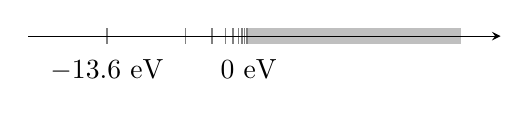
\begin{tikzpicture}[baseline={($ (current bounding box.center)- (0,-6pt) $)}]
\foreach \i in {1,2,...,9,10}{
\draw[gray] (3-2/\i,0.1) -- (3-2/\i,-0.1);
}
\fill[lightgray]  (2.79,0.1) rectangle (5.5,-0.1);
\draw[->] (0,0)--(6,0);
\draw (1,-0.1) node[below=2pt]{$-13.6$ eV};
\draw (2.8,-0.1) node[below=2pt]{$0$ eV};
\end{tikzpicture}
\ei
Note that one of the parts may actually be empty. For instance, as we will later show, the simple quantum harmonic oscillator has the following energy spectrum 
\bi{rCl}
\sigma(H) & =\ & 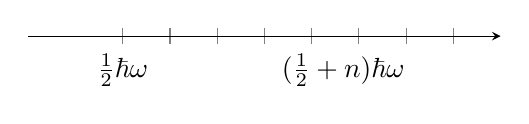
\begin{tikzpicture}[baseline={($ (current bounding box.center)- (0,-7.5pt) $)}]
\foreach \i in {2,...,9}{
\draw[gray] (0.6*\i,0.1) -- (0.6*\i,-0.1);
}
\draw (1.2,-0.1) node[below]{$\tfrac{1}{2}\hbar \omega$};
\draw (4,-0.1) node[below]{$(\tfrac{1}{2}+n)\hbar \omega$};
\draw[->] (0,0)--(6,0);
\end{tikzpicture}
\ei
while the spectrum of the position operator $Q$ is $\sigma(Q) =  \R$.

Also, the continuous part need not be connected, as is the case with spectrum of the Hamiltonian an electron in a periodic potential
\bi{rCl}
\sigma(H) & =\ & 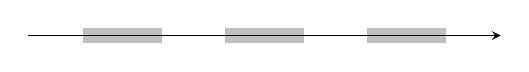
\begin{tikzpicture}
\foreach \i in {0,1,2}{
\fill[lightgray]  (1.8*\i,0.1) rectangle (1+1.8*\i,-0.1);
}
\draw[->] (-0.7,0)--(5.3,0);
\end{tikzpicture}
\ei
It turns out that self-adjoint linear maps on a complex Hilbert space provide a suitable formalism to describe the observables of quantum mechanics. 
\item \textit{An irreducible impact that each measurement has on the state of a quantum system.}

The crucial example demonstrating this is the Stern-Gerlach experiment\index{Stern-Gerlach experiment}, which consists in the following. Silver atoms are heated up in an oven and sent against a screen with a hole. The atoms passing through the hole are then subjected to an inhomogeneous magnetic field, which deflects them according to the component of their angular momentum in the direction of the field. Finally, a screen detects the various deflections.

\begin{center}
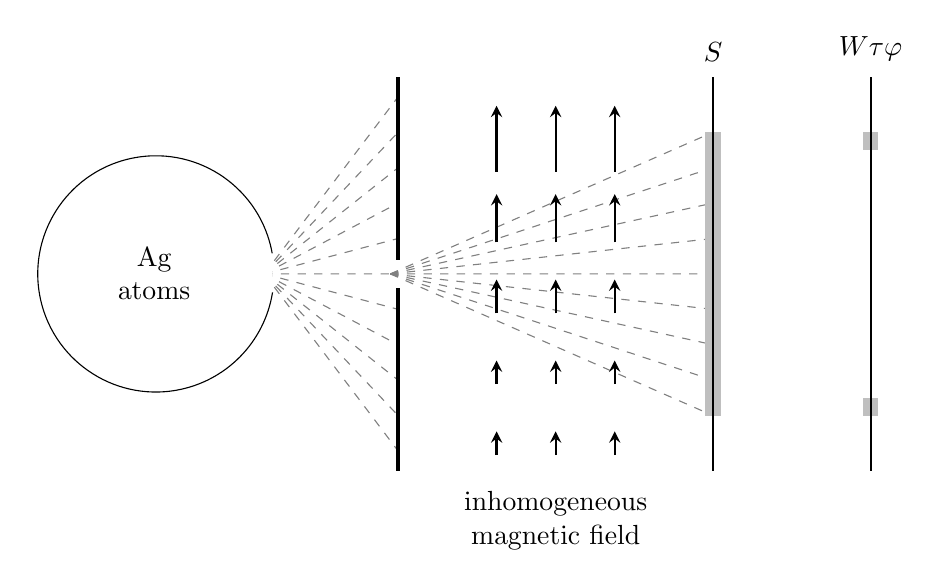
\begin{tikzpicture}[every text node part/.style={align=center}]
\foreach \i in {0,1,...,10} {
\draw[dashed,gray] (0.8,0) -- (2.5,2.25-0.45*\i);
};
\draw[fill=white] (0.9,1.5*sin 10) arc (10:351:1.5);

\draw[ultra thick] (2.5,2.5)--(2.5,0.18);
\draw[ultra thick] (2.5,-0.18)--(2.5,-2.5);
\draw (-0.6,0)  node {Ag\\ atoms};

\foreach \i in {1,...,9} {
\draw[dashed,gray] (2.4,0) -- (6.5,2.25-0.45*\i);
};

\foreach \i in {0,1,...,4} {
  \foreach \j in {1,2,3} {
\draw[thick,->] (3+0.75*\j,-2.3+0.9*\i) -- (3+0.75*\j,-2+0.9*\i^1.1);
};};

\fill[lightgray] (6.5-0.1,2.25-0.45*9) rectangle (6.5+0.1,2.25-0.45);
\draw[thick] (6.5,-2.5)--(6.5,2.5) node[above=2pt] {$S$};

\fill[lightgray] (8.5-0.1,2.25-0.45*9) rectangle (8.5+0.1,2.25-8.5*0.45);
\fill[lightgray] (8.5-0.1,2.25-0.45*1.5) rectangle (8.5+0.1,2.25-0.45);
\draw[thick] (8.5,-2.5)--(8.5,2.5) node[above=2pt] {$W\tau\varphi$};
\draw (4.5,-2.5) node[below=4pt] {inhomogeneous \\ magnetic field};
\end{tikzpicture}
\end{center}

Since the angular momentum distribution of the silver atoms coming from the oven is random, we would expect an even distribution of values of the component along the direction of the magnetic field to be recorded on the final screen, as in $S$. However, the impact pattern actually detected is that on the $W\tau\varphi$ screen. In fact, 50\% of the incoming atoms impact at the top and we say that their angular momentum component is $\uparrow$, and the other 50\% hit the bottom region, and we say that their angular momentum component is $\downarrow$.  This is another instance of our earlier point: there seem to be only two possible values for the component of angular momentum along the direction of the magnetic field, i.e.\ the spectrum is discrete. Hence, this is not particularly surprising at this point.

Let us now consider successive iterations of this experiment. Introduce some system of cartesian coordinates $(x,y,z)$ and let $\mathrm{SG}(x)$ and $\mathrm{SG}(z)$ denotes a Stern-Gerlach apparatus whose magnetic field points in the $x$ and $z$-direction, respectively.

Suppose that we sent the atoms through a first $\mathrm{SG}(z)$ apparatus, and then we use the $z^\uparrow$-output as the input of a second $\mathrm{SG}(z)$ apparatus.
\begin{center}
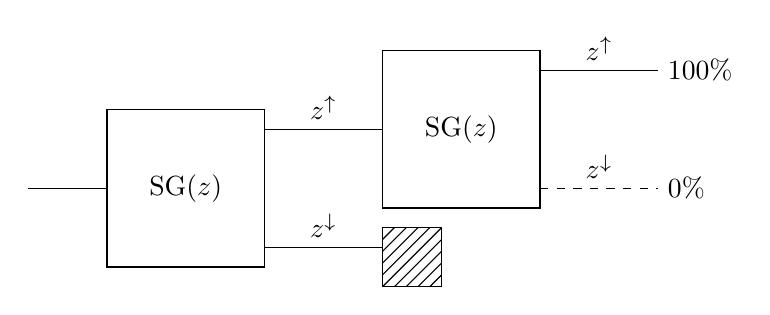
\begin{tikzpicture}[scale=0.5]
\draw (-2,2) -- (0,2);
\draw (2,2) node {$\mathrm{SG}(z)$};
\draw  (0,0) rectangle (4,4);
\draw (4,3.5) -- (7,3.5) node[above,midway] {$z^\uparrow$};
\draw (4,0.5) -- (7,0.5) node[above,midway] {$z^\downarrow$};
\draw  (7,1.5) rectangle (11,5.5);
\draw  (7,1) rectangle (8.5,-0.5);
\draw  (11,5) -- (14,5)  node[above,midway] {$z^\uparrow$} node[right] {100\%};
\draw[dashed]  (11,2) -- (14,2) node[above,midway] {$z^\downarrow$} node[right] {0\%};
\node at (9,3.5) {$\mathrm{SG}(z)$};
\foreach \i in {1,...,5} {
\draw (7+0.3*\i,1)--(7,1-0.3*\i);
\draw (7+0.3*\i,-0.5)--(8.5,1-0.3*\i);
};
\end{tikzpicture}
\end{center}
The second $\mathrm{SG}(z)$ apparatus finds no $z^\downarrow$-atoms. This is not surprising since, intuitively, we ``filtered out'' all the $z^\downarrow$-atoms with the first apparatus. Suppose now that we feed the $z^\uparrow$ output of a $\mathrm{SG}(z)$ apparatus into a $\mathrm{SG}(x)$ apparatus.

\begin{center}
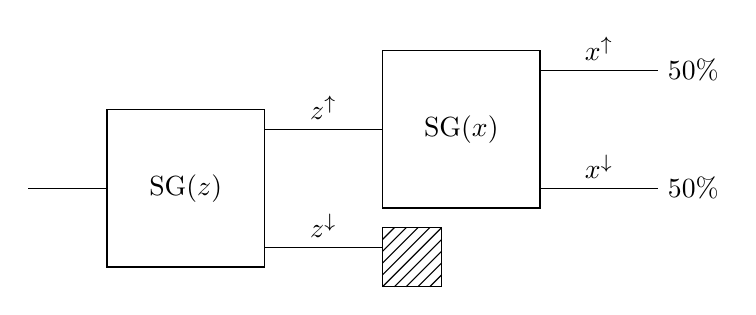
\begin{tikzpicture}[scale=0.5]
\draw (-2,2) -- (0,2);
\draw (2,2) node {$\mathrm{SG}(z)$};
\draw  (0,0) rectangle (4,4);
\draw (4,3.5) -- (7,3.5) node[above,midway] {$z^\uparrow$};
\draw (4,0.5) -- (7,0.5) node[above,midway] {$z^\downarrow$};
\draw  (7,1.5) rectangle (11,5.5);
\draw  (7,1) rectangle (8.5,-0.5);
\draw  (11,5) -- (14,5)  node[above,midway] {$x^\uparrow$} node[right] {50\%};
\draw  (11,2) -- (14,2) node[above,midway] {$x^\downarrow$} node[right] {50\%};
\node at (9,3.5) {$\mathrm{SG}(x)$};
\foreach \i in {1,...,5} {
\draw (7+0.3*\i,1)--(7,1-0.3*\i);
\draw (7+0.3*\i,-0.5)--(8.5,1-0.3*\i);
};
\end{tikzpicture}
\end{center}
Experimentally, we find that about half of the atoms are detected in the state $x^\uparrow$ and half in the state $x^\downarrow$. This is, again, not surprising since we only filtered out the $z^\uparrow$ atoms, and hence we can interpret this result as saying that the $x^\uparrow$, $x^\downarrow$ states are independent from the $z^\uparrow$, $z^\downarrow$.

If our ideas of ``filtering states out'' is correct, then feeding the $x^\uparrow$-output of the previous set-up to another $\mathrm{SG}(z)$ apparatus should clearly produce a $100\%$ $z^\uparrow$-output, since we already filtered out all the $z^\downarrow$ ones in the previous step.

\begin{center}
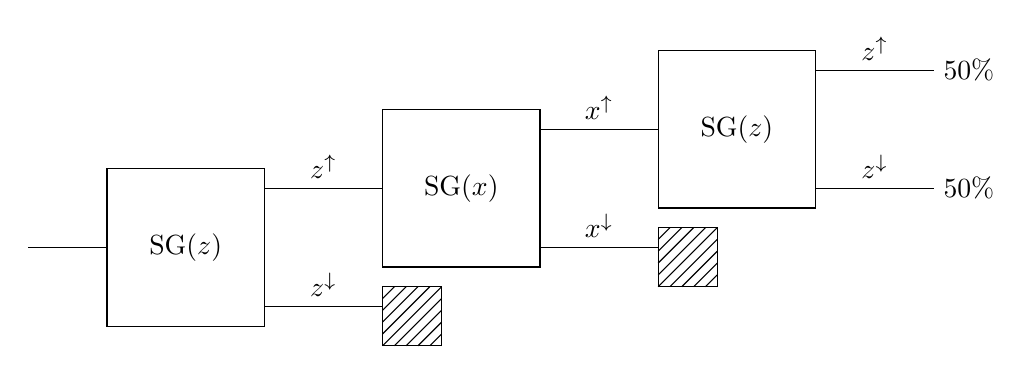
\begin{tikzpicture}[scale=0.5]
\draw (-2,2) -- (0,2);
\draw (2,2) node {$\mathrm{SG}(z)$};
\draw  (0,0) rectangle (4,4);
\draw (4,3.5) -- (7,3.5) node[above,midway] {$z^\uparrow$};
\draw (4,0.5) -- (7,0.5) node[above,midway] {$z^\downarrow$};
\draw  (7,1.5) rectangle (11,5.5);
\draw  (11,5) -- (14,5)  node[above,midway] {$x^\uparrow$} ;
\draw  (11,2) -- (14,2) node[above,midway] {$x^\downarrow$};
\node at (9,3.5) {$\mathrm{SG}(x)$};
\draw  (7,1) rectangle (8.5,-0.5);
\foreach \i in {1,...,5} {
\draw (7+0.3*\i,1)--(7,1-0.3*\i);
\draw (7+0.3*\i,-0.5)--(8.5,1-0.3*\i);
};

\draw  (14,2.5) rectangle (15.5,1);
\foreach \i in {1,...,5} {
\draw (14+0.3*\i,2.5)--(14,2.5-0.3*\i);
\draw (14+0.3*\i,2-1)--(15.5,2.5-0.3*\i);
};
\draw  (14,3) rectangle (18,7);
\draw (16,5) node {$\mathrm{SG}(z)$};
\draw (18,6.5) -- (21,6.5) node[above,midway] {$z^\uparrow$} node[right] {50\%};
\draw (18,3.5) -- (21,3.5) node[above,midway] {$z^\downarrow$} node[right] {50\%};
\end{tikzpicture}
\end{center}
Surprisingly, the output is again $50$-$50$. The idea behind this result is the following. The $\mathrm{SG}(z)$ apparatus left the atoms in a state such that a repeated measurement with the $\mathrm{SG}(z)$ apparatus would give the same result, and similarly for the $\mathrm{SG}(x)$ apparatus. However, the measurement of the $\mathrm{SG}(x)$ apparatus somehow altered the state of the atoms in such a way as to ``reset'' them with respect to a measurement by the $\mathrm{SG}(z)$ apparatus. For more details on the Stern-Gerlach experiment and  further conclusions one can draw from its results, you should consult the book \textit{Modern Quantum Mechanics} by J. J. Sakurai. The conclusion that we are interested in here is that measurements can alter the state of a system.

\item \textit{Even if the state $\rho$ of a quantum system is completely known, the only prediction one can make for the measurement of some observable $A$ is the probability that the measured valued, which is an element of the spectrum $\sigma(A)$, lies within a Borel-measurable subset $E\subseteq \R$, denoted by
$\mu^A_{\rho}(E)$}.

In particular, one cannot predict which concrete outcome an isolated measurement will produce. This is even more annoying given that the precise impact that a measurement has on the state of the system (see previous point) depends on the observed outcome of the measurement.
\een

A suitable theory that accommodates all known experimental facts has been developed between 1900 and 1927 on the physics side by, among others, Schr\"odinger, Heisenberg and Dirac, and on the mathematical side almost single-handedly by von Neumann who invented a massive proportion of a field known today as functional analysis.

\subsection{The axioms of quantum mechanics}

We will now present the axioms of quantum mechanics by using notions and terminology that will be defined later in the course. In this sense, this section constitutes a preview of the next few lectures. 

\begin{tcolorbox}[colframe=blue!10!black,before skip=10pt,after skip=10pt]
\begin{axiom}[Quantum systems and states]
To every quantum system there is associated a separable complex Hilbert space $(\mathcal{H},+,\cdot,\langle \cdot | \cdot \rangle)$. The states of the system are all positive, trace-class linear maps $\rho\cl \mathcal{H}\to \mathcal{H}$ for which $\Tr\rho=1$.
\end{axiom}
\end{tcolorbox}

\br
Throughout the quantum mechanics literature, it is stated that the unit, or normalised, elements $\psi\in\mathcal{H}$ (that is, $\langle\psi|\psi\rangle=1$) are the states of the quantum system. This is not correct. 

States can be pure or mixed. A state $\rho\cl \mathcal{H}\to \mathcal{H}$ is called \emph{pure} if
\bse
\exists \, \psi\in \mathcal{H} : \forall \, \alpha\in \mathcal{H} : \ \rho(\alpha) = \frac{\langle\psi|\alpha\rangle}{\langle\psi|\psi\rangle}\psi.
\ese
Thus, we can associate to each pure state $\rho$ an element $\psi\in\mathcal{H}$. However, this correspondence is not one-to-one. Even if we restrict to pure states and impose the normalisation condition, there can be many $\psi\in\mathcal{H}$ representing the same pure state $\rho$. 

Therefore, it is wrong to say that the states of the states of the quantum system are the normalised elements of the Hilbert space, since they do not represent all the states of the system, and do not even represent uniquely the states that they do represent.
\er

The terms used in Axiom 1 are defined as follows.

\bd
A \emph{complex Hilbert space}\index{Hilbert space} is a tuple $(\mathcal{H},+,\cdot,\langle \cdot | \cdot \rangle)$ where
\begin{itemize}
\item $\mathcal{H}$ is a set
\item $+$ is a map $+\cl\mathcal{H}\times \mathcal{H}\to \mathcal{H}$
\item $\cdot$ is a map $\cdot \cl \C \times \mathcal{H}\to \mathcal{H}$ (typically suppressed in the notation)
\end{itemize}
such that the triple $(\mathcal{H},+,\cdot)$ is a vector space over $\C$, and
\begin{itemize}
\item $\langle \cdot | \cdot \rangle$ is a \emph{sesqui-linear\footnote{sesqui is Latin for ``one and a half''.}inner product}, i.e.\ a map $\langle \cdot | \cdot \rangle\cl\mathcal{H}\times \mathcal{H}\to \mathcal{H}$ satisfying
\ben[label=(\roman*)]
\item $\langle \varphi|\psi\rangle=\overline{\langle \psi|\varphi\rangle}$\hfill (conjugate symmetry/Hermitian property)
\item $\langle \varphi|z\psi_1+\psi_2\rangle=z\langle \varphi|\psi_1\rangle+\langle \varphi|\psi_2\rangle$ \hfill (linearity in the second argument)
\item $\langle \psi | \psi\rangle \geq 0$ and $\langle \psi|\psi\rangle = 0 \Leftrightarrow \psi = 0$ \hfill (positive-definiteness)
\een
for all $\varphi,\psi_1,\psi_2\in\mathcal{H}$ and $z\in \C$,
\end{itemize}
and moreover
\begin{itemize}
\item $\mathcal{H}$ is a \emph{complete metric space} with respect to the metric induced by the norm induced in turn by the sesqui-linear map $\langle \cdot | \cdot \rangle$. Explicitly, for every sequence $\phi\cl \N \to \mathcal{H}$ that satisfies the \emph{Cauchy property}, namely
\bse
\forall \, \varepsilon > 0 : \exists \, N\in \N : \forall \, n,m \geq N : \ \|\phi_n-\phi_m\|< \varepsilon,
\ese
where $\phi_n:=\phi(n)$ and $\|\psi\|:=\sqrt{\langle \psi | \psi \rangle}$, then the sequence converges in $\mathcal{H}$, i.e.\
\bse
\exists \, \varphi\in\mathcal{H}:\forall \, \varepsilon > 0 : \exists \, N\in \N : \forall \, n \geq N : \ \|\varphi-\phi_n\|< \varepsilon.
\ese
\end{itemize}
\ed
Note that the $\C$-vector space $(\mathcal{H},+,\cdot)$ need not be finite-dimensional and, in fact, we will mostly work with infinite-dimensional Hilbert spaces. 

\bd
A map $A\cl\mathcal{D}_A\to \mathcal{H}$, where the subspace $\mathcal{D}_A\subseteq \mathcal{H}$ is called the \emph{domain} of $A$, is a \emph{linear map} if
\bse
\forall \, \varphi,\psi\in\mathcal{D}_A:\forall \, z \in \C : \ A(z\varphi+\psi)=zA(\varphi)+A(\psi).
\ese
\ed
From now on, if there is no risk of confusion, we will write $A\varphi:=A(\varphi)$ in order to spare some brackets. We will be particularly interested in special types of linear map.


% \bd
% A linear map $A\cl\mathcal{D}_A\to \mathcal{H}$ is said to be
% \begin{itemize}
% \item \emph{densely defined} if $\mathcal{D}_A$ is \emph{dense} in $\mathcal{H}$, i.e.\
% \bse
% \forall \, \psi\in \mathcal{H} : \exists \, \alpha \in \mathcal{D}_A : \forall \, \varepsilon >0 :\ \|\alpha-\psi\|<\varepsilon
% \ese
% \item \emph{positive} if 
% \bse
% \forall \, \psi\in\mathcal{D}_A : \ \langle\psi|A\psi\rangle\geq 0
% \ese
% \item of \emph{trace-class} if $\mathcal{D}_A=\mathcal{H}$ and, for any orthonormal basis $\{e_n\}$ of $\mathcal{H}$, the sum/series
% \bse
% \sum_n \langle e_n|Ae_n\rangle < \infty.
% \ese
% \end{itemize}
% \ed


\bd
A linear map $A\cl\mathcal{D}_A\to \mathcal{H}$ is \emph{densely defined} if $\mathcal{D}_A$ is \emph{dense} in $\mathcal{H}$, i.e.\
\bse
\forall \, \psi\in \mathcal{H} : \forall \, \varepsilon >0: \exists \, \alpha \in \mathcal{D}_A  :\ \|\alpha-\psi\|<\varepsilon.
\ese
\ed

\bd
A linear map $A\cl\mathcal{D}_A\to \mathcal{H}$ is said to be \emph{positive} if 
\bse
\forall \, \psi\in\mathcal{D}_A : \ \langle\psi|A\psi\rangle\geq 0.
\ese
\ed


\bd
A linear map $A\cl\mathcal{D}_A\to \mathcal{H}$ is said to be of \emph{trace-class} if $\mathcal{D}_A=\mathcal{H}$ and, for any orthonormal basis $\{e_n\}$ of $\mathcal{H}$, the sum/series
\bse
\sum_n \langle e_n|Ae_n\rangle < \infty.
\ese
\ed
If $A\cl\mathcal{H}\to \mathcal{H}$ is of trace-class, one can show that the value of $\sum_n \langle e_n|Ae_n\rangle$ does not depend on the choice of orthonormal basis $\{e_n\}$. 
\bd
Let $A\cl\mathcal{H}\to \mathcal{H}$ be of trace-class. Then the \emph{trace} of $A$ is
\bse
\Tr A :=\sum_n \langle e_n|Ae_n\rangle 
\ese
where $\{e_n\}$ is any orthonormal basis of $\mathcal{H}$.
\ed
\begin{tcolorbox}[colframe=blue!10!black]
\begin{axiom}[Observables]
The observables of a quantum system are the self-adjoint linear maps $A\cl\mathcal{D}_A\to \mathcal{H}$.
\end{axiom}
\end{tcolorbox}
While the notion of a self-adjoint map is easy to define in finite-dimensional spaces, it is much more subtle for infinite-dimensional spaces.

\bd
A densely defined linear map $A\cl\mathcal{D}_A\to \mathcal{H}$ is said to be of \emph{self-adjoint} if it coincides with its adjoint map $A^*\cl\mathcal{D}_{A^*}\to \mathcal{H}$, that is
\begin{itemize}
\item $\mathcal{D}_A=\mathcal{D}_{A^*}$
\item $\forall \, \varphi\in\mathcal{D}_A : \ A\varphi=A^*\varphi$.
\end{itemize}
\ed
%The subtle part is the definition of the adjoint map itself.
\bd
The \emph{adjoint map} $A^*\cl\mathcal{D}_{A^*}\to \mathcal{H}$ of a linear map $A\cl\mathcal{D}_A\to \mathcal{H}$ is defined by
\begin{itemize}
\item $\mathcal{D}_{A^*}:=\{\psi\in\mathcal{H}\mid \forall \, \alpha \in \mathcal{D}_A:\exists \, \eta \in \mathcal{H} : \langle\psi|A\alpha\rangle=\langle\eta|\alpha\rangle\}$
\item $A^*\psi:=\eta$.
\end{itemize}
\ed
We will later show that the adjoint map is well-defined, i.e.\ for each $\alpha\in\mathcal{D}_A$ and $\psi\in\mathcal{H}$ there exists at most one $\eta\in\mathcal{H}$ such that $\langle\psi|A\alpha\rangle = \langle\eta|\alpha\rangle$.

\br
If we defined $\mathcal{D}_{A^*}$ by requiring that $\eta\in \mathcal{D}_{A}$, we would obtain a notion of self-adjointness which has undesirable properties. In particular, the spectrum (to be defined later) of a self-adjoint operator would not be guaranteed to be a subset of $\R$.
\er

\begin{tcolorbox}[colframe=blue!10!black]
\begin{axiom}[Measurement]
The probability that a measurement of an observable $A$ on a system that is in the state $\rho$ yields a result in the Borel set $E\subseteq \R$ is given by
\bse
\mu^A_\rho(E):=\Tr(\mathrm{P}_{\!A}(E)\circ\rho)
\ese
where the map $\mathrm{P}_{\!A}\cl \Borel(\R)\to\mathcal{L}(\mathcal{H})$, from the Borel-measurable subsets of $\R$ to the Banach space of bounded linear maps on $\mathcal{H}$, is the unique projection-valued measure that is associated with the self-adjoint map $A$ according to the spectral theorem.\end{axiom}\end{tcolorbox}

We will later see that the composition of a bounded linear map with a trace-class map is again of trace-class, so that $\Tr(\mathrm{P}_{\!A}(E)\circ\rho)$ is well-defined. For completeness, the spectral theorem states that for any self-adjoint map $A$ there exists a projection-valued measure $\mathrm{P}_{\!A}$ such that $A$ can be represented in terms of the Lebesgue-Stieltjes integral as
\bse
A = \int_{\R}\lambda \, \d \mathrm{P}_{\!A}(\lambda).
\ese
This is the infinite-dimensional analogue of the diagonalisation theorem for symmetric or Hermitian matrices on finite-dimensional vector spaces, and it is the theorem in which the first half of the course will find its climax.


\begin{tcolorbox}[colframe=blue!10!black,before skip=10pt]
\begin{axiom}[Unitary dynamics]
In a time interval $(t_1,t_2)\subseteq \R$ in which no measurement occurs, the state $\rho$ at time $t_1$, denoted $\rho(t_1)$, is related to the state $\rho$ at time $t_2$, denoted $\rho(t_2)$, by
\bse
\rho(t_2) = \mathcal{U}(t_2-t_1)\rho(t_1)\mathcal{U}^{-1}(t_2-t_1)
\ese
with the unitary evolution operator $\mathcal{U}$ defined as
\bse
\mathcal{U}(t) := \exp(-\tfrac{\mathrm{i}}{\hbar}Ht),
\ese
where $H$ is the energy observable and, for any observable $A$ and $f\cl \R\to \C$, we define
\bse
f(A):=\int_\R f(\lambda) \, \d \mathrm{P}_{\!A}(\lambda).
\ese
\end{axiom}
\end{tcolorbox}
Note that, as was the case for the previous axiom, the spectral theorem is crucial since it is needed to define  the unitary evolution operator.

\begin{tcolorbox}[colframe=blue!10!black,before skip=10pt]
\begin{axiom}[Projective dynamics]
The state $\rho_{\mathrm{after}}$ of a quantum system immediately following the measurement of an observable $A$ is
\bse
\rho_{\mathrm{after}} := \frac{\mathrm{P}_{\!A}(E)\circ\rho_{\mathrm{before}}\circ\mathrm{P}_{\!A}(E)}{\Tr(\mathrm{P}_{\!A}(E)\circ\rho_{\mathrm{before}}\circ\mathrm{P}_{\!A}(E))}
\ese
where $\rho_{\mathrm{before}}$ is the state immediately preceding the measurement and $E\subseteq\R$ is the smallest Borel set in which the actual outcome of the measurement happened to lie.
\end{axiom}
\end{tcolorbox}
























\newpage

\section{Banach spaces}

Hilbert spaces are a special type of a more general class of spaces known as Banach spaces. We are interested in Banach spaces not just for the sake generality, but also because they naturally appear in Hilbert space theory. For instance, the space of bounded linear maps on a Hilbert space is not itself a Hilbert space, but only a Banach space.

\subsection{Generalities on Banach spaces}

We begin with some basis notions from metric space theory.

\bd
A \emph{metric space}\index{metric space} is a pair $(X,d)$, where $X$ is a set and $d$ is a \emph{metric} on $X$, that is, a map $d\cl X\times X \to \R$ satisfying
\ben[label=(\roman*)]
\item $d(x,x)\geq 0$ \hfill (non-negativity)
\item $d(x,y) = 0\ \Leftrightarrow \ x=y$ \hfill (identity of indiscernibles)
\item $d(x,y)=d(y,x)$ \hfill (symmetry)
\item $d(x,z)\leq d(x,y)+d(y,z)$ \hfill (triangle inequality)
\een
for all $x,y,z\in X$.
\ed

\bd
A sequence $\{x_n\}_{n\in \N}$ in a metric space $(X,d)$ is said to \emph{converge}\index{convergence} to an element $x\in X$, written $\displaystyle \lim_{n\to \infty}x_n=x$, if
\bse
\forall \, \varepsilon > 0 : \exists \, N \in \N : \forall \, n \geq N : \ d(x_n,x)<\varepsilon.
\ese
\ed

A sequence in a metric space can converge to at most one element.

\bd
A \emph{Cauchy sequence}\index{Cauchy sequence} in a metric space $(X,d)$ is a sequence $\{x_n\}_{n\in \N}$ such that
\bse
\forall \, \varepsilon > 0 : \exists \, N \in \N : \forall \, n,m \geq N : \ d(x_n,x_m)<\varepsilon.
\ese
\ed
Any convergent sequence is clearly a Cauchy sequence.

\vbox{\bd
A metric space $(X,d)$ is said to be \emph{complete}\index{completeness} if every Cauchy sequence converges to some $x\in X$.
\ed
A natural metric on a vector space is that induced by a norm.
\bd
A \emph{normed space}\index{normed space} is a (complex) vector space $(V,+,\cdot)$ equipped with a \emph{norm}, that is, a map $\|\cdot\|\cl V \to \R$ satisfying
\ben[label=(\roman*)]
\item $\|f\|\geq 0$ \hfill (non-negativity)
\item $\|f\| = 0 \ \Leftrightarrow\ f=0$ \hfill (definiteness)
\item $\|z\cdot f\|=|z|\|f\|$ \hfill (homogeneity/scalability)
\item $\|f+g\|\leq \|f\|+\|g\|$ \hfill (triangle inequality/sub-additivity)
\een
for all $f,g\in V$ and all $z\in \C$.
\ed}
One we have a norm $\|\cdot\|$ on $V$, we can define a metric $d$ on $V$ by 
\bse
d(f,g) := \|f-g\|.
\ese
Then we say that the normed space $(V,\|\cdot\|)$ is \emph{complete} if the metric space $(V,d)$, where $d$ is the metric induced by $\|\cdot\|$, is complete. Note that we will usually suppress inessential information in the notation, for example writing $(V,\|\cdot\|)$ instead of $(V,+,\cdot,\|\cdot\|)$.

\bd
A \emph{Banach space}\index{Banach space} is a complete normed vector space.
\ed

\be
The space $C^0_\C[0,1]:=\{f\cl [0,1]\to \C \mid f \text{ is continuous}\}$, where the continuity is with respect to the standard topologies on $[0,1]\subset \R$ and $\C$, is a Banach space. Let us show this in some detail.
\bq
\ben[label=(\alph*)]
\item First, define two operations $+,\cdot$ pointwise, that is, for any $x\in [0,1]$
\bse
(f+g)(x) := f(x)+g(x)\qquad \quad (z\cdot f)(x):=zf(x).
\ese
Suppose that $f,g\in C^0_\C[0,1]$, that is
\bse
\forall \, x_0\in [0,1]: \forall \, \varepsilon > 0 : \exists \, \delta > 0 : \forall \, x\in (x_0-\delta,x_0+\delta) : \ |f(x)-f(x_0)|<\varepsilon
\ese
and similarly for $g$. Fix $x_0\in[0,1]$ and $\varepsilon >0$. Then, there exist $\delta_1,\delta_2>0$ such that
\bi{c}
\forall \, x\in (x_0-\delta_1,x_0+\delta_1) : \ |f(x)-f(x_0)|<\tfrac{\varepsilon}{2}\phantom{.}\\
\forall \, x\in (x_0-\delta_2,x_0+\delta_2) : \ |g(x)-g(x_0)|<\tfrac{\varepsilon}{2}.
\ei
Let $\delta:=\min\{\delta_1,\delta_2\}$. Then, for all $x\in (x_0-\delta,x_0+\delta)$, we have
\bi{rCl}
|(f+g)(x)-(f+g)(x_0)| & := & |f(x)+g(x)-(f(x_0)+g(x_0))|\\
 & = & |f(x)-f(x_0)+g(x)-g(x_0))|\\
 & \leq & |f(x)-f(x_0)|+|g(x)-g(x_0))|\\
& < & \tfrac{\varepsilon}{2}+\tfrac{\varepsilon}{2}\\
& = & \varepsilon.
\ei
Since $x_0\in[0,1]$ was arbitrary, we have $f+g\in C^0_\C[0,1]$. Similarly, for any $z\in \C$ and $f\in C^0_\C[0,1]$, we also have $z\cdot f\in C^0_\C[0,1]$. It is immediate to check that the complex vector space structure of $\C$ implies that the operations
\bi{rrClcrrCl}
+\cl & C^0_\C[0,1] \times C^0_\C[0,1] & \to & C^0_\C[0,1] &\quad \qquad & \cdot \cl &\C \times C^0_\C[0,1] & \to & C^0_\C[0,1]\\
& (f,g) &\mapsto & f+g && & (z,f) & \mapsto & z\cdot f
\ei
make $(C^0_\C[0,1],+,\cdot)$ into a complex vector space.

\item Since $[0,1]$ is closed and bounded, it is compact and hence every complex-valued continuous function $f\cl [0,1]\to \C$ is bounded, in the sense that
\bse
\sup_{x\in[0,1]}|f(x)| < \infty.
\ese
We can thus define a norm on $C^0_\C[0,1]$, called the \emph{supremum} (or \emph{infinity}) \emph{norm}, by
\bse
\|f\|_{\infty} := \sup_{x\in[0,1]}|f(x)| .
\ese
Let us show that this is indeed a norm on $(C^0_\C[0,1],+,\cdot)$ by checking that the four defining properties hold. Let $f,g\in C^0_\C[0,1]$ and $z\in \C$. Then
\ben[label=(b.\roman*)]
\item $\displaystyle \|f\|_{\infty}:= \sup_{x\in[0,1]}|f(x)| \geq 0$ since $|f(x)|\geq 0$ for all $x\in [0,1]$.
\item $\displaystyle \|f\|_{\infty}=0\ \Leftrightarrow \sup_{x\in[0,1]}|f(x)| = 0$. By definition of supremum, we have
\bse
\forall \, x \in [0,1] : \ |f(x)|\leq \sup_{x\in[0,1]}|f(x)| = 0. 
\ese
But since we also have $|f(x)|\geq 0$ for all $x\in [0,1]$, $f$ is identically zero.
\item $\displaystyle \|z\cdot f\|_{\infty} := \sup_{x\in[0,1]}|zf(x)| = \sup_{x\in[0,1]}|z||f(x)|=|z|\sup_{x\in[0,1]}|f(x)| = |z|\|f\|_{\infty}$.
\item By using the triangle inequality for the modulus of complex numbers, we have
\bi{rCl}
\|f+g\|_{\infty} &:=& \sup_{x\in[0,1]}|(f+g)(x)|\\
&=& \sup_{x\in[0,1]}|f(x)+g(x)|\\
&\leq & \sup_{x\in[0,1]}(|f(x)|+|g(x)|)\\
& = & \sup_{x\in[0,1]}|f(x)|\,+\sup_{x\in[0,1]}|g(x)|\\
& = & \|f\|_{\infty}+\|g\|_{\infty}.
\ei
Hence, $(C^0_\C[0,1],\|\cdot\|_{\infty})$ is indeed a normed space.
\een
\item We now show that $C^0_\C[0,1]$ is complete. Let $\{f_n\}_{n\in \N}$ be a Cauchy sequence of functions in $C^0_\C[0,1]$, that is
\bse
\forall \, \varepsilon > 0 : \exists \, N \in \N : \forall \, n,m \geq N : \ \|f_n-f_m\|_{\infty} <\varepsilon.
\ese
We seek an $f\in C^0_\C[0,1]$ such that $\displaystyle \lim_{n\to\infty}f_n=f$. We will proceed in three steps.
\ben[label=(c.\roman*)]
\item Fix $y\in [0,1]$ and $\varepsilon >0$. By definition of supremum, we have
\bse
f_n(y) -f_m(y) \leq \sup_{x\in[0,1]}|f_n(x)-f_m(x)| =: \|f_n-f_m\|_{\infty}.
\ese
Hence, there exists $N\in \N$ such that
\bse
\forall \, n,m \geq N : \ f_n(y) -f_m(y)<\varepsilon,
\ese
that is, the sequence of complex numbers $\{f_n(y)\}_{n\in \N}$ is a Cauchy sequence. Since $\C$ is a complete metric space\footnote{The standard metric on $\C$ is induced by the modulus of complex numbers.}, there exists $z_y\in\C$ such that $\displaystyle \lim_{n\to \infty}f_n(y)=z_y$. 

Thus, we can define a function
\bi{rrCl}
f\cl & [0,1] & \to & \C\\
& x & \mapsto & z_x,
\ei
called the \emph{pointwise limit} of $f$, which by definition satisfies
\bse
\forall \, x \in [0,1] : \ \lim_{n\to \infty}f_n(x)=f(x).
\ese
Note that this does \emph{not} automatically imply that $\displaystyle \lim_{n\to \infty}f_n=f$ (converge with respect to the supremum norm), nor that $f\in C^0_\C[0,1]$, and hence we need to check separately that these do, in fact, hold.
\item First, let us check that $f\in C^0_\C[0,1]$, that is, $f$ is continuous. Let $x_0\in [0,1]$ and $\varepsilon>0$. For each $x\in [0,1]$, we have
\bi{rCl}
|f(x)-f(x_0)| & = & |f(x)-f_n(x)+f_n(x)-f_n(x_0)+f_n(x_0)-f(x_0)|\\
 & \leq & |f(x)-f_n(x)|+|f_n(x)-f_n(x_0)|+|f_n(x_0)-f(x_0)|.
\ei
Since $f$ is the pointwise limit of $\{f_n\}_{n\in\N}$, for each $x\in[0,1]$ there exists $N\in \N$ such that
\bse
\forall \, n \geq N : \ |f(x)-f_n(x)|<\tfrac{\varepsilon}{3}.
\ese
In particular, we also have
\bse
\forall \, n \geq N : \ |f_n(x_0)-f(x_0)|<\tfrac{\varepsilon}{3}.
\ese
Moreover, since $f_n\in C^0_\C[0,1]$ by assumption, there exists $\delta>0$ such that
\bse
\forall \, x\in (x_0-\delta,x_0+\delta)  : \ |f_n(x)-f_n(x_0)|<\tfrac{\varepsilon}{3}.
\ese
Fix $n\geq N$. Then, it follows that for all $x\in (x_0-\delta,x_0+\delta)$, we have
\bi{rCl}
|f(x)-f(x_0)|  & \leq & |f(x)-f_n(x)|+|f_n(x)-f_n(x_0)|+|f_n(x_0)-f(x_0)|\\
& < & \tfrac{\varepsilon}{3}+\tfrac{\varepsilon}{3}+\tfrac{\varepsilon}{3}\\
& = & \varepsilon.
\ei
Since $x_0\in[0,1]$ was arbitrary, we have $f\in C^0_\C[0,1]$.
\item Finally, it remains to show that $\displaystyle \lim_{n\to \infty}f_n=f$. To that end, let $\varepsilon>0$. By the triangle inequality for $\|\cdot\|_{\infty}$, we have
\bi{rCl}
\|f_n-f\|_{\infty} &=& \|f_n-f_m+f_m-f\|_{\infty}\\
&\leq& \|f_n-f_m\|_{\infty}+\|f_m-f\|_{\infty}.
\ei
Since $\{f_n\}_{n\in\N}$ is Cauchy by assumption, there exists $N_1\in \N$ such that
\bse
\forall \, n,m\geq N : \ \|f_n-f_m\|_{\infty} < \tfrac{\varepsilon}{2}.
\ese
Moreover, since $f$ is the pointwise limit of $\{f_n\}_{n\in\N}$, for each $x\in[0,1]$ there exists $N_2\in \N$ such that
\bse
\forall \, m \geq N_2 : \ |f_m(x)-f(x)|<\tfrac{\varepsilon}{2}.
\ese
By definition of supremum, we have
\bse
\forall \, m \geq N_2 : \ \|f_m-f\|_{\infty}= \sup_{x\in[0,1]}|f_m(x)-f(x)|\leq\tfrac{\varepsilon}{2}.
\ese
Let $N:=\max\{N_1,N_2\}$ and fix $m\geq N$. Then, for all $n\geq N$, we have
\bi{c}
\|f_n-f\|_{\infty} \leq \|f_n-f_m\|_{\infty}+\|f_m-f\|_{\infty} < \tfrac{\varepsilon}{2} + \tfrac{\varepsilon}{2} = \varepsilon.
\ei
Thus, $\displaystyle \lim_{n\to \infty}f_n = f$ and we call $f$ the \emph{uniform limit} of $\{f_n\}_{n\in\N}$.
\een
\een
This completes the proof that $(C^0_\C[0,1],\|\cdot\|_{\infty})$ is a Banach space.
\eq
\ee

\br
The previous example shows that checking that something is a Banach space, and the completeness property in particular, can be quite tedious. However, in the following, we will typically already be working with a Banach (or Hilbert) space and hence, rather than having to check that the completeness property holds, we will instead be able to use it to infer the existence (within that space) of the limit of any Cauchy sequence.
\er

\subsection{Bounded linear operators}

As usual in mathematics, once we introduce a new types of structure, we also want study maps between instances of those structures, with extra emphasis placed on the structure-preserving maps. We begin with linear maps from a normed space to a Banach space.

\bd
Let $(V,\|\cdot\|_V)$ be a normed space and $(W,\|\cdot\|_W)$ a Banach space. A linear map, also called a linear operator, $A\cl V\to W$ is said to be \emph{bounded} if
\bse
\sup_{f\in V}\frac{\|Af\|_W}{\|f\|_V} < \infty.
\ese
\ed
Note that the quotient is not defined for $f=0$. Hence, to be precise, we should write $V\setminus\{0\}$ instead of just $V$. Let us agree that is what mean in the above definition. There are several equivalent characterisations of the boundedness property.

\vbox{
\bp
\label{prp:boundequiv}
A linear operator $A\cl V\to W$ is bounded if, and only if, any of the following conditions are satisfied.
\ben[label=(\roman*)]
\item $\displaystyle \sup_{\|f\|_V=1}\|Af\|_W< \infty$
\item $\exists \, k > 0 : \forall \, f\in V: \ \|f\|_V \leq 1\, \Rightarrow \, \|Af\|_W \leq k$
\item $\exists \, k > 0 : \forall \, f\in V: \ \|Af\|_W\leq  k \|f\|_V$
\item the map $A\cl V \to W$ is continuous with respect to the topologies induced by the respective norms on $V$ and $W$
\item the map $A$ is continuous at $0\in V$. 
\een
\ep}

The first one of these follows immediately from the homogeneity of the norm. Indeed, suppose that $\|f\|_V\neq 1$. Then
\bse
\frac{\|Af\|_W}{\|f\|_V} = \|f\|_V^{-1}\|Af\|_W =\|A(\|f\|_V^{-1} f)\|_W = \|A\widetilde f\|_W 
\ese
where $\widetilde f:= \|f\|_V^{-1}f$ is such that $\|\widetilde f\|_V=1$. Hence, the boundedness property is equivalent to condition (i) above. 

\bd
Let $A\cl V \to W$ be a bounded operator. The \emph{operator norm}\index{operator norm} of $A$ is defined as
\bse
\|A\|:=\sup_{\|f\|_V=1} \|Af\|_W = \sup_{f\in V}\frac{\|Af\|_W}{\|f\|_V} .
\ese
\ed

\be
Let $\id_W\cl W\to W$ be the identity operator on a Banach space $W$. Then
\bse
\sup_{\|f\|_W=1}\|\id_Wf\|_W =\sup_{\|f\|_W=1}\|f\|_W = 1 <\infty.
\ese
Hence, $\id_W$ is a bounded operator and has unit norm.
\ee

\be
Denote by $C^1_{\C}[0,1]$ the complex vector space of once continuously differentiable complex-valued functions on $[0,1]$. Since differentiability implies continuity, this is a subset of $C^0_{\C}[0,1]$. Moreover, since sums and scaling by a complex number of continuously differentiable functions are again continuously differentiable, this is, in fact, a vector subspace of $C^0_{\C}[0,1]$, and hence also a normed space with the supremum norm $\|\cdot\|_{\infty}$.

Consider the first derivative operator
\bi{rrCl}
D \cl & C^1_{\C}[0,1] & \to & C^0_{\C}[0,1]\\
& f & \mapsto & f'.
\ei
We know from undergraduate real analysis that $D$ is a linear operator. We will now show that $D$ is an unbounded\footnote{Some people take the term unbounded to mean ``not necessarily bounded''. We take it to mean ``definitely not bounded'' instead.} linear operator. That is,
\bse
\sup_{f\in C^1_{\C}[0,1]} \frac{\|Df\|_{\infty}}{\|f\|_{\infty}} = \infty.
\ese
Note that, since the norm is a function into the real numbers, both $\|Df\|_{\infty}$ and $\|f\|_{\infty}$ are always finite for any $f\in C^1_{\C}[0,1]$. Recall that the supremum of a set of real numbers is its least upper bound and, in particular, it need not be an element of the set itself. What we have to show is that the set
\bse
\biggl\{ \frac{\|Df\|_{\infty}}{\|f\|_{\infty}} \ \Big| \ f\in C^1_{\C}[0,1] \biggr\} \subset \R
\ese
contains arbitrarily large elements. One way to do this is to exhibit a positively divergent (or unbounded from above) sequence within the set. 

Consider the sequence $\{f_n\}_{n\geq 1}$ where $f_n(x):=\sin(2\pi nx)$. We know that sine is continuously differentiable, hence $f_n\in C^1_{\C}[0,1]$ for each $n\geq 1$, with
\bse
Df_n(x) = D(\sin(2\pi nx)) = 2\pi n\cos(2\pi nx).
\ese
We have
\bse
\|f_n\|_{\infty} = \sup_{x\in[0,1]}|f_n(x)| = \sup_{x\in[0,1]}|\sin(2\pi nx)| = \sup \, [-1,1] = 1 
\ese
and
\bse
\|Df_n\|_{\infty} = \sup_{x\in[0,1]}|Df_n(x)| = \sup_{x\in[0,1]}|2\pi n\cos(2\pi nx)| = \sup\, [-2\pi n,2\pi n] = 2\pi n.
\ese
Hence, we have
\bse
\sup_{f\in C^1_{\C}[0,1]} \frac{\|Df\|_{\infty}}{\|f\|_{\infty}} \geq \sup_{\{f_n\}_{n\geq 1}} \frac{\|Df\|_{\infty}}{\|f\|_{\infty}} = \sup_{n\geq 1}\,2\pi n = \infty,
\ese
which is what we wanted. As an aside, we note that $C^1_{\C}[0,1]$ is not complete with respect to the supremum norm, but it is complete with respect to the norm
\bse
\|f\|_{C^1}:=\|f\|_{\infty}+\|f'\|_{\infty}.
\ese
While the derivative operator is still unbounded with respect to this new norm, in general, the boundedness of a linear operator does depend on the choice of norms on its domain and target, as does the numerical value of the operator norm.
\ee

\br
Apart from the ``minor'' detail that in quantum mechanics we deal with Hilbert spaces, use a different norm than the supremum norm and that the (one-dimensional) momentum operator acts as $P(\psi):=-\mathrm{i}\hbar\psi'$, the previous example is a harbinger of the fact that the momentum operator in quantum mechanics is unbounded. This will be the case for the position operator $Q$ as well.
\er
\bl
\label{lem:forcompl}
Let $(V,\|\cdot\|)$ be a normed space. Then, addition, scalar multiplication, and the norm are all sequentially continuous. That is, for any sequences $\{f_n\}_{n\in \N}$ and $\{g_n\}_{n\in \N}$ in $V$ converging to $f\in V$ and $g\in V$ respectively, and any sequence $\{z_n\}_{n\in \N}$ in $\C$ converging to $z\in \C$, we have
\ben[label=(\roman*)]
\item $\displaystyle \lim_{n\to \infty}(f_n+g_n)=f+g$
\item $\displaystyle \lim_{n\to \infty}z_nf_n=zf$.
\item $\displaystyle \lim_{n\to \infty}\|f_n\|=\|f\|$
\een
\el

\bq
\ben[label=(\roman*)]
\item Let $\varepsilon >0$. Since $\displaystyle \lim_{n\to \infty}f_n=f$ and $\displaystyle \lim_{n\to \infty}g_n=g$ by assumption, there exist $N_1,N_2\in \N$ such that
\bi{c}
\forall \, n\geq N_1 : \ \|f-f_n\|<\tfrac{\varepsilon}{2}\phantom{.}\\
\forall \, n\geq N_2 : \ \|g-g_n\|<\tfrac{\varepsilon}{2}.
\ei
Let $N:=\max\{N_1,N_2\}$. Then, for all $n\geq N$, we have
\bi{rCl}
\|(f_n+g_n)-(f+g)\| &=& \|f_n-f+g_n-g\|\\
&\leq& \|f_n-f\|+\|g_n-g\|\\
& < & \tfrac{\varepsilon}{2}+\tfrac{\varepsilon}{2}\\
& = & \varepsilon.
\ei
Hence $\displaystyle \lim_{n\to \infty}(f_n+g_n)=f+g$.


\item Since $\{z_n\}_{n\in \N}$ is a convergent sequence in $\C$, it is bounded. That is,
\bse
\exists \, k>0 : \forall \, n\in \N : \ |z_n|\leq k.
\ese
Let $\varepsilon >0$. Since $\displaystyle \lim_{n\to \infty}f_n=f$ and $\displaystyle \lim_{n\to \infty}z_n=z$, there exist $N_1,N_2\in \N$ such that
\bi{l}
\forall \, n\geq N_1 : \ \|f-f_n\|<\frac{\varepsilon}{2k}\\
\forall \, n\geq N_2 : \ \|z-z_n\|<\frac{\varepsilon}{2\|f\|}.
\ei
Let $N:=\max\{N_1,N_2\}$. Then, for all $n\geq N$, we have
\bi{rCl}
\|z_nf_n-zf\| &=& \|z_nf_n-z_nf+z_nf-zf\|\\
&=& \|z_n(f_n-f)+(z_n-z)f\|\\
&\leq& \|z_n(f_n-f)\|+\|(z_n-z)f\|\\
&=& |z_n|\|f_n-f\|+|z_n-z|\|f\|\\
& < & k\frac{\varepsilon}{2k}+\frac{\varepsilon}{2\|f\|}\|f\|\\
& = & \varepsilon.
\ei
Hence $\displaystyle \lim_{n\to \infty}z_nf_n=zf$.
\item Let $\varepsilon >0$. Since  $\displaystyle \lim_{n\to \infty}f_n=f$, there exists $N\in \N$ such that
\bse
\forall \, n \geq N : \ \|f_n-f\|<\varepsilon.
\ese
By the triangle inequality, we have
\bse
\|f_n\| = \|f_n-f+f\| \leq \|f_n-f\|+\|f\|  
\ese
so that $\|f_n\|-\|f\|\leq \|f_n-f\|$. Similarly, $\|f\|-\|f_n\|\leq \|f-f_n\|$. Since
\bse
\|f-f_n\| = \|-(f_n-f)\| = |-1|\|f_n-f\| = \|f_n-f\|,
\ese
we have $-\|f_n-f\|\leq\|f_n\|-\|f\|\leq\|f_n-f\|$ or, by using the modulus,
\bse
\bigl| \|f_n\|-\|f\|\bigr| \leq \|f_n-f\|.
\ese
Hence, for all $n\geq N$, we have $\bigl| \|f_n\|-\|f\|\bigr| <\varepsilon$ and thus  $\displaystyle \lim_{n\to \infty}\|f_n\|=\|f\|$.
\qedhere
\een
\eq
Note that by taking $\{z_n\}_{n\in\N}$ to be the constant sequence whose terms are all equal to some fixed $z\in \C$, we have $\displaystyle \lim_{n\to \infty}zf_n=zf$ as a special case of (ii).

This lemma will take care of some of the technicalities involved in proving the following crucially important result.

\begin{theorem}
The set $\mathcal{L}(V,W)$ of bounded linear operators from a normed space $(V,\|\cdot\|_V)$ to a Banach space $(W,\|\cdot\|_W)$, equipped with pointwise addition and scalar multiplication and the operator norm, is a Banach space.
\end{theorem}

\bq
\ben[label=(\alph*)]
\item Define addition and scalar multiplication on $\mathcal{L}(V,W)$ by
\bse
(A+B)f := Af+Bf \quad \qquad (zA)f := zAf.
\ese
It is clear that both $A+B$ and $zA$ are linear operators.  Moreover, we have
\bi{rCl}
\sup_{f\in V}\frac{\|(A+B)f\|_W}{\|f\|_V} &:=& \sup_{f\in V}\frac{\|Af+Bf\|_W}{\|f\|_V} \\
 &\leq & \sup_{f\in V}\frac{\|Af\|_W+\|Bf\|_W}{\|f\|_V} \\
 &=& \sup_{f\in V}\frac{\|Af\|_W}{\|f\|_V} + \sup_{f\in V}\frac{\|Bf\|_W}{\|f\|_V} \\
 &<& \infty
\ei
since $A$ and $B$ are bounded. Hence, $A+B$ is also bounded and we have
\bse
\|A+B\|\leq \|A\|+\|B\|.
\ese
Similarly, for $zA$ we have 
\bi{rCl}
\sup_{f\in V}\frac{\|(zA)f\|_W}{\|f\|_V} &:=& \sup_{f\in V}\frac{\|zAf\|_W}{\|f\|_V} \\
 &= & \sup_{f\in V}\frac{|z|\|Af\|_W}{\|f\|_V} \\
 &=& |z|\sup_{f\in V}\frac{\|Af\|_W}{\|f\|_V} \\
 &<& \infty
\ei
since $A$ is bounded and $|z|$ is finite. Hence, $zA$ is bounded and we have
\bse
\|zA\|=|z|\|A\|.
\ese
Thus, we have two operations
\bi{rrClcrrCl}
+\cl & \mathcal{L}(V,W)\times \mathcal{L}(V,W) & \to & \mathcal{L}(V,W) &\qquad \quad & \cdot \cl & \C \times \mathcal{L}(V,W) & \to & \mathcal{L}(V,W)\\
& (A,B) & \mapsto & A+B && & (z,A) & \mapsto & zA
\ei
and it is immediate to check that the vector space structure of $W$ induces a vector space structure on $\mathcal{L}(V,W)$ with these operations.

\item We need to show that $(\mathcal{L}(V,W),\|\cdot\|)$ is a normed space, i.e.\ that $\|\cdot\|$ satisfies the properties of a norm. We have already shown two of these in part (a), namely
\ben[label=(b.\roman*),start=3]
\item $\|zA\|=|z|\|A\|$
\item $\|A+B\|\leq \|A\|+\|B\|$.
\een
The remaining two are easily checked.
\ben[label=(b.\roman*)]
\item $\displaystyle \|A\|:=\sup_{f\in V}\frac{\|Af\|_W}{\|f\|_V}\geq 0$ since $\|\cdot\|_V$ and $\|\cdot\|_W$ are norms.
\item Again, by using the fat that $\|\cdot\|_W$ is a norm,
\bi{rCl"s}
\|A\|=0 &\ \Leftrightarrow\ & \sup_{f\in V}\frac{\|Af\|_W}{\|f\|_V}= 0\\
& \Leftrightarrow & \forall \, f\in V:\ \|Af\|_W=0\\
& \Leftrightarrow & \forall \, f\in V:\ Af=0\\
& \Leftrightarrow & \ A=0.
\ei
\een
Hence, $(\mathcal{L}(V,W),\|\cdot\|)$ is a normed space.

\item The heart of the proof is showing that $(\mathcal{L}(V,W),\|\cdot\|)$ is complete. We will proceed in three steps, analogously to the case of $C_{\C}^0[0,1]$.
\ben[label=(c.\roman*)]
\item Let $\{A_n\}_{n\in \N}$ be a Cauchy sequence in $\mathcal{L}(V,W)$. Fix $f\in V$ and let $\varepsilon >0$. Then, there exists $N\in \N$ such that
\bse
\forall \, n,m\geq N : \ \|A_n-A_m\|<\frac{\varepsilon}{\|f\|_V}.
\ese
Then, for all $n,m\geq N$, we have
\bi{rCl}
\|A_nf-A_mf\|_W & = & \|(A_n-A_m)f\|_W\\
& = & \|f\|_V\frac{\|(A_n-A_m)f\|_W}{\|f\|_V}\\
& \leq & \|f\|_V\sup_{f\in V}\frac{\|(A_n-A_m)f\|_W}{\|f\|_V}\\
& =: & \|f\|_V\|A_n-A_m\|\\
& < & \|f\|_V \frac{\varepsilon}{\|f\|_V}\\
& = & \varepsilon.
\ei
(Note that if $f=0$, we simply have $\|A_nf-A_mf\|_W=0<\varepsilon$ and, in the future, we will not mention this case explicitly.) Hence, the sequence $\{A_nf\}_{n\in \N}$ is a Cauchy sequence in $W$. Since $W$ is a Banach space, the limit $\lim_{n\to \infty}A_nf$ exists and is an element of $W$. Thus, we can define the operator
\bi{rrCl}
A\cl & V & \to & W\\
& f & \mapsto & \lim_{n\to \infty}A_nf,
\ei
called the pointwise limit of $\{A_n\}_{n\in \N}$.
\item We now need to show that $A\in \mathcal{L}(V,W)$. This is where the previous lemma comes in handy. For linearity, let $f,g\in V$ and $z\in \C$. Then
\bi{rCl}
A(zf+g) &:=& \lim_{n\to \infty} A_n(zf+g)\\
& = & \lim_{n\to \infty} (zA_nf+A_ng)\\
& = & z\lim_{n\to \infty} A_nf+\lim_{n\to \infty}A_ng\\
&=:& zAf+Ag
\ei
where we have used the linearity of each $A_n$ and part (i) and (ii) of \Cref{lem:forcompl}.
For boundedness, part (ii) and (iii) of \Cref{lem:forcompl} yield
\bi{rCl}
\|Af\|_W  & = & \lim_{n\to \infty} \|A_nf\|_W\\
& = & \lim_{n\to \infty} \|f\|_V\frac{\|A_nf\|_W}{\|f\|_V}\\
& \leq & \lim_{n\to \infty} \|f\|_V\sup_{f\in V}\frac{\|A_nf\|_W}{\|f\|_V}\\
& = & \|f\|_V \lim_{n\to \infty} \|A_n\|
\ei
for any $f\in V$. By rearranging, we have
\bse
\forall\, f\in V:\ \frac{\|Af\|_W}{\|f\|_V} \leq  \lim_{n\to \infty} \|A_n\|.
\ese
Hence, to show that $A$ is bounded, it suffices to show that the limit on the right hand side is finite. Let $\varepsilon > 0$. Since $\{A_n\}_{n\in \N}$ is a Cauchy sequence, there exists $N\in \N$ such that
\bse
\forall \, n,m \geq N : \ \|A_n-A_m\|<\varepsilon.
\ese
Then, by the proof of part (i) of \Cref{lem:forcompl}, we have
\bse
\bigl| \|A_n\|-\|A_m\|\bigr| \leq  \|A_n-A_m\|<\varepsilon
\ese
for all $n,m \geq N$. Hence, the sequence of real numbers $\{\|A_n\|\}_{n\in \N}$ is a Cauchy sequence. Since $\R$ is complete, this sequence converges to some real number $\ell\in\R$. Therefore
\bse
\sup_{f\in V} \frac{\|Af\|_W}{\|f\|_V} \leq  \lim_{n\to \infty} \|A_n\| = \ell < \infty
\ese
and thus $A\in \mathcal{L}(V,W)$.

\item To conclude, we have to show that $\displaystyle \lim_{n\to\infty}A_n=A$. Let $\varepsilon >0$. Then
\bi{c}
\|A_n-A\| = \|A_n+A_m-A_m-A\| \leq \|A_n-A_m\|+ \|A_m-A\|.  
\ei
Since $\{A_n\}_{n\in \N}$ is Cauchy, there exists $N_1\in \N$ such that
\bse
\forall \, n,m\geq N_1 : \ \|A_n-A_m\| < \tfrac{\varepsilon}{2}.
\ese
Moreover, since $A$ is the pointwise limit of $\{A_n\}_{n\in \N}$, for any $f\in V$ there exists $N_2\in \N$ such that
\bse
\forall \, m\geq N_2 : \ \|A_mf-Af\|_W < \frac{\varepsilon\|f\|_V}{2}
\ese
and hence, for all $m\geq N_2$
\bse
\|A_m-A\| := \sup_{f\in V}\frac{\|A_mf-Af\|_W}{\|f\|_V} \leq \frac{\tfrac{\varepsilon\|f\|_V}{2}}{\|f\|_V} = \frac{\varepsilon}{2} 
\ese
Let $N:=\max\{N_1,N_2\}$ and fix $m\geq N$. Then, for all $n\geq N$, we have
\bse
\|A_n-A\| \leq \|A_n-A_m\|+ \|A_m-A\| <\tfrac{\varepsilon}{2}+\tfrac{\varepsilon}{2}=\varepsilon. 
\ese
Thus, $\displaystyle \lim_{n\to\infty}A_n=A$ and we call $A$ the uniform limit of $\{A_n\}_{n\in \N}$.
\een
\een
This concludes the proof that $(\mathcal{L}(V,W),\|\cdot\|)$ is a Banach space.
\eq

\br
Note that if $V$ and $W$ are normed spaces, then $\mathcal{L}(V,W)$ is again a normed space, while for $\mathcal{L}(V,W)$ to be a Banach space it suffices that $W$ be a Banach space.
\er

\br
In the proof that $\mathcal{L}(V,W)$ is a Banach space, we have shown a useful inequality which we restate here for further emphasis. If $A\cl V\to W$ is bounded, then 
\bse
\forall \, f\in V :\ \|Af\|_W\leq\|A\|\|f\|_V
\ese
\er

The following is an extremely important special case of $\mathcal{L}(V,W)$.

\bd
Let $V$ be a normed space. Then $V^*:=\mathcal{L}(V,\C)$ is called the \emph{dual}\index{dual} of $V$.
\ed

Note that, since $\C$ is a Banach space, the dual of a normed space is a Banach space. The elements of $V^*$ are variously called \emph{covectors} or \emph{functionals} on $V$. 
\br
You may recall from undergraduate linear algebra that the dual of a vector space was defined to be the vector space of \emph{all} linear maps $V\to\C$, rather than just the bounded ones. This is because, in finite dimensions, all linear maps are bounded. So the two definitions agree as long as we are in finite dimensions. If we used the same definition for the infinite-dimensional case, then $V^*$ would lack some very desirable properties, such as that of being a Banach space.
\er
The dual space can be used to define a weaker notion of convergence called, rather unimaginatively, weak convergence. 

\bd
A sequence $\{f_n\}_{n\in \N}$ is said to \emph{converge weakly}\index{weak convergence} to $f\in V$ if
\bse
\forall \, \varphi\in V^* : \lim_{n\to\infty}\varphi(f_n) = \varphi(f).
\ese
\ed

Note that $\{\varphi(f_n)\}_{n\in \N}$ is just a sequence of complex numbers. To indicate that the sequence $\{f_n\}_{n\in \N}$ converges weakly to $f\in V$ we write
\bse
\wlim_{n\to \infty} f_n = f.
\ese
In order to further emphasise the distinction with weak convergence, we may say that $\{f_n\}_{n\in \N}$ converges \emph{strongly} to $f\in V$ if it converges according to the usual definition, and we will write accordingly
\bse
\slim_{n\to \infty} f_n = f.
\ese

\bp
Let $\{f_n\}_{n\in \N}$ be a sequence in a normed space $(V,\|\cdot\|_V)$. If $\{f_n\}_{n\in \N}$ converges strongly to $f\in V$, then it also converges weakly to $f\in V$, i.e.\
\bse
\slim_{n\to \infty} f_n = f \quad \Rightarrow \quad \wlim_{n\to \infty} f_n = f.
\ese
\ep

\bq
Let $\varepsilon >0$ and let $\varphi\in V^*$. Since $\{f_n\}_{n\in \N}$ converges strongly to $f\in V$, there exists $N\in\N$ such that
\bse
\forall \, n\geq N : \ \|f_n-f\|_V<\frac{\varepsilon}{\|\varphi\|}.
\ese
Then, for any $n\geq N$, we have
\bi{rCl}
\|\varphi f_n-\varphi f\|_W & = & \|\varphi ( f_n-f)\|_W\\
& \leq & \|\varphi\|\|f_n-f\|_V\\
&<& \|\varphi\|\frac{\varepsilon}{\|\varphi\|}\\
& = & \varepsilon
\ei
since $\varphi$ is bounded. Hence, $\displaystyle  \lim_{n\to \infty} \varphi(f_n) = \varphi(f)$. That is, $\displaystyle  \wlim_{n\to \infty} f_n = f$.
\eq

\subsection{Extension of bounded linear operators}

Note that, so far, we have only considered bounded linear maps $A\cl\mathcal{D}_A\to W$ where $\mathcal{D}_A$ is the whole of $V$, rather than a subspace thereof. The reason for this is that we will only consider densely defined linear maps in general, and any bounded linear map from a dense subspace of $V$ can be extended to a bounded linear map from the whole of $V$. Moreover, the extension is unique. This is the content of the so-called BLT\footnote{Bounded Linear Transformation, \emph{not} Bacon, Lettuce, Tomato. \begin{tikzpicture}[baseline={($ (current bounding box.center)- (0,-7pt) $)}]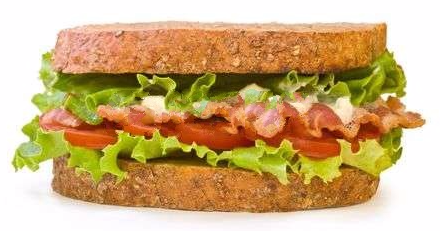
\includegraphics[scale=0.12]{graphics/blt}\end{tikzpicture}} theorem.

\bl
Let $(V,\|\cdot\|)$ be a normed space and let $\mathcal{D}_A$ be a dense subspace of $V$. Then, for any $f\in V$, there exists a sequence $\{\alpha_n\}_{n\in \N}$ in $\mathcal{D}_A$ which converges to $f$.
\el
\bq
Let $f\in V$. Clearly, there exists a sequence $\{f_n\}_{n\in \N}$ in $V$ which converges to $f$ (for instance, the constant sequence). Let $\varepsilon >0$. Then, there exists $N\in \N$ such that
\bse
\forall \, n\geq N : \ \|f_n-f\| < \tfrac{\varepsilon}{2}.
\ese
Since $\mathcal{D}_A$ is dense in $V$ and each $f_n\in V$, we have
\bse
\forall \, n\in \N : \exists\, \alpha_n\in\mathcal{D}_A : \ \|\alpha_n-f_n\|<\tfrac{\varepsilon}{2}.\\[7pt]
\ese
The sequence $\{\alpha_n\}_{n\in \N}$ is a sequence in $\mathcal{D}_A$ and we have
\bi{rCl}
\|\alpha_n-f\|&=&\|\alpha_n-f_n+f_n-f\|\\
&\leq &\|\alpha_n-f_n\|+\|f_n-f\| \\
&<&\tfrac{\varepsilon}{2}+\tfrac{\varepsilon}{2}\\
&=&\varepsilon
\ei
for all $n\geq N$. Hence $\displaystyle \lim_{n\to\infty}\alpha_n=f$.
\eq

\bd
Let $V,W$ be vector spaces and let $A\cl\mathcal{D}_A\to W$ be a linear map, where $\mathcal{D}_A\subseteq V$. An \emph{extension}\index{extension} of $A$ is a linear map $\widehat A\cl V\to W$ such that
\bse
\forall \, \alpha\in \mathcal{D}_A : \ \widehat A \alpha = A\alpha.
\ese
\ed

\bt[BLT theorem]
Let $V$ be a normed space and $W$ a Banach space. Any densely defined linear map $A\cl\mathcal{D}_A\to W$ has a unique extension $\widehat A\cl V\to W$ such that $\widehat A$ is bounded. Moreover, $\|{\widehat A}\|=\|A\|$.
\et

\bq
\ben[label=(\alph*)]
\item Let $A\in \mathcal{L}(\mathcal{D}_A,W)$. Since $\mathcal{D}_A$ is dense in $V$, for any $f\in V$ there exists a sequence $\{\alpha_n\}_{n\in \N}$ in $\mathcal{D}_A$ which converges to $f$. Moreover, since $A$ is bounded, we have 
\bse
\forall \, n\in \N : \ \|A\alpha_n-A\alpha_m\|_W \leq \|A\| \|\alpha_n-\alpha_m\|_V,
\ese
from which it quickly follows that $\{A\alpha_n\}_{n\in \N}$ is Cauchy in $W$. As $W$ is a Banach space, this sequence converges to an element of $W$ and thus we can define
\bi{rrCl}
\widehat A \cl & V &\to & W\\
& f & \mapsto & \lim_{n\to\infty}A\alpha_n,
\ei
where $\{\alpha_n\}_{n\in \N}$ is any sequence in $\mathcal{D}_A$ which converges to $f$.
\item First, let us show that $\widehat A$ is well-defined. Let $\{\alpha_n\}_{n\in \N}$ and $\{\beta_n\}_{n\in \N}$ be two sequences in $\mathcal{D}_A$ which converge to $f\in V$ and let $\varepsilon > 0$. Then, there exist $N_1,N_2\in \N$ such that
\bi{c}
\forall \, n\geq N_1 : \ \|\alpha_n-f\|_V < \frac{\varepsilon}{2\|A\|}\\
\forall \, n\geq N_2 : \ \|\beta_n-f\|_V < \frac{\varepsilon}{2\|A\|}.
\ei
Let $N:=\max\{N_1,N_2\}$. Then, for all $n\geq N$, we have
\bi{rCl}
\|A\alpha_n-A\beta_n\|_W & = & \|A(\alpha_n-\beta_n)\|_W\\
&\leq & \|A\| \| \alpha_n-\beta_n\|_V\\
& = & \|A\| \| \alpha_n-f+f-\beta_n\|_V\\
&\leq & \|A\| (\| \alpha_n-f\|_V+\|f-\beta_n\|_V)\\
&< & \|A\| \Bigl(\frac{\varepsilon}{2\|A\|}+\frac{\varepsilon}{2\|A\|}\Bigr)\\
&=&\varepsilon,
\ei
where we have used the fact that $A$ is bounded. Thus, we have shown
\bse
\lim_{n\to\infty}(A\alpha_n-A\beta_n) = 0.
\ese
Then, by using \Cref{lem:forcompl} and rearranging, we find
\bse
\lim_{n\to\infty}A\alpha_n = \lim_{n\to\infty}A\beta_n,
\ese
that is, $\widehat A$ is indeed well-defined.

\item To see that $\widehat A$ is an extension of $A$, let $\alpha\in\mathcal{D}_A$. The constant sequence $\{\alpha_n\}_{n\in \N}$ with $\alpha_n=\alpha$ for all $n\in \N$ is a sequence in $\mathcal{D}_A$ converging to $\alpha$. Hence
\bse
\widehat A \alpha := \lim_{n\to\infty} A\alpha_n =  \lim_{n\to\infty} A\alpha = A\alpha.
\ese

\item We now check that $A\in\mathcal{L}(V,W)$. For linearity, let $f,g\in V$ and $z\in \C$. As $\mathcal{D}_A$ is dense in $V$, there exist sequences $\{\alpha_n\}_{n\in \N}$ and $\{\beta_n\}_{n\in \N}$ in $\mathcal{D}_A$ converging to $f$ and $g$, respectively. Moreover, as $\mathcal{D}_A$ is a subspace of $V$, the sequence $\{\gamma_n\}_{n\in \N}$ given by
\bse
\gamma_n:=z\alpha_n+\beta_n
\ese
is again a sequence in $\mathcal{D}_A$ and, by \Cref{lem:forcompl}, 
\bse
\lim_{n\to\infty}\gamma_n = zf+g.
\ese
Then, we have
\bi{rCl}
\widehat A (zf+g) &:=& \lim_{n\to\infty} A\gamma_n \\
&=& \lim_{n\to\infty}A(z\alpha_n+\beta_n)\\
&=& \lim_{n\to\infty}(zA\alpha_n+A\beta_n)\\
&=& z\lim_{n\to\infty}A\alpha_n+\lim_{n\to\infty}A\beta_n\\
&=:& z\widehat A f+\widehat Ag .
\ei
For boundedness, let $f\in V$ and $\{\alpha_n\}_{n\in \N}$ a sequence in $\mathcal{D}_A$ which converges to $f$. Then, since $A$ is bounded,
\bi{rCl}
\|\widehat A f\|_W &:=& \bigl\|\lim_{n\to\infty}A\alpha_n\bigr\|_W\\
 &=& \lim_{n\to\infty}\|A\alpha_n\|_W\\
 & \leq &\lim_{n\to\infty}\|A\|\|\alpha_n\|_V\\
 & = &\|A\|\lim_{n\to\infty}\|\alpha_n\|_V\\
 & = &\|A\|\|f\|_V.
\ei
Therefore
\bse
\sup_{f\in V} \frac{\|\widehat A f\|_W}{\|f\|_V} \leq \sup_{f\in V} \frac{\|A\|\|f\|_V}{\|f\|_V} =\sup_{f\in V} \|A\| =\|A\| < \infty
\ese
and hence $\widehat A$ is bounded.
\item For uniqueness, suppose that $\widetilde A\in\mathcal{L}(V,W)$ is another extension of $A$. Let $f\in V$ and $\{\alpha_n\}_{n\in \N}$ a sequence in $\mathcal{D}_A$ which converges to $f$. Then, we have
\bse
\|\widetilde A f - A\alpha_n\|_W = \|\widetilde A f - \widetilde A\alpha_n\|_W \leq  \|\widetilde A\| \|f-\alpha_n\|_V .
\ese
It follows that
\bse
\lim_{n\to\infty}(\widetilde A f - A\alpha_n) = 0
\ese
and hence, for all $f\in V$,
\bse
\widetilde Af = \lim_{n\to\infty} A\alpha_n =: \widehat A f.
\ese
Therefore, $\widetilde A = \widehat A$.
\item Finally, we have already shown in part (d) that
\bse
\|\widehat A\|:=\sup_{f\in V} \frac{\|\widehat A f\|_W}{\|f\|_V} \leq \|A\|.
\ese
On the other hand, since $\mathcal{D}_A\subseteq V$, we must also have
\bse
\|A\|:=\sup_{f\in \mathcal{D}_A} \frac{\| A f\|_W}{\|f\|_V} = \sup_{f\in \mathcal{D}_A} \frac{\|\widehat A f\|_W}{\|f\|_V} \leq \sup_{f\in V} \frac{\|\widehat A f\|_W}{\|f\|_V}=: \|\widehat A\|.
\ese
Hence, we also have $\|A\|\leq\|\widehat A\|$. Thus, $\|\widehat A\|=\|A\|$.\qedhere
\een
\eq

\br
Note a slight abuse of notation in the equality $\|\widehat A\|=\|A\|$. The linear maps $\widehat A$ and $A$ belong to $\mathcal{L}(V,W)$ and $\mathcal{L}(\mathcal{D}_A,W)$, respectively. These are different normed (in fact, Banach) spaces and, in particular, carry \emph{different} norms. To be more precise, we should have written
\bse
\|\widehat A\|_{\mathcal{L}(V,W)} = \|A\|_{\mathcal{L}(\mathcal{D}_A,W)},
\ese
where 
\bse
\|\widehat A\|_{\mathcal{L}(V,W)} := \sup_{f\in V} \frac{\| \widehat A f\|_W}{\|f\|_V} \qquad \text{and}\qquad
\| A\|_{\mathcal{L}(\mathcal{D}_A,W)} := \sup_{f\in \mathcal{D}_A} \frac{\| A f\|_W}{\|f\|_V}.
\ese
\er






















\newpage

\section{Separable Hilbert Spaces}


\subsection{Relationship between norms and inner products}

A Hilbert space is a vector space $(\mathcal{H},+,\cdot)$ equipped with a sesqui-linear inner product $\langle\cdot|\cdot\rangle$ which induces a norm $\|\cdot\|_{\mathcal{H}}$ with respect to which $\mathcal{H}$ is a Banach space. Note that by ``being induced by $\langle\cdot|\cdot\rangle$'' we specifically mean that the norm is defined as
\bi{rrCl}
\|\cdot\|\cl & V & \to & \R\\
& f & \mapsto & \sqrt{\langle f|f\rangle}.
\ei

Recall that a sesqui-linear inner product on $\mathcal{H}$ is a map $\langle\cdot|\cdot\rangle\cl \mathcal{H} \times \mathcal{H} \to \mathcal{H}$ which is conjugate symmetric, linear in the second argument and positive-definite. Note that conjugate symmetry together with linearity in the second argument imply conjugate linearity in the first argument:
\bi{rCl}
\langle z\psi_1+\psi_2|\varphi\rangle & = & \overline{\langle \varphi| z\psi_1+\psi_2\rangle }\\
& = & \overline{z\langle \varphi| \psi_1\rangle+\langle \varphi| \psi_2\rangle }\\
& = & \overline{z}\overline{\langle \varphi| \psi_1\rangle}+\overline{\langle \varphi| \psi_2\rangle }\\
& = & \overline{z}\langle \psi_1|\varphi\rangle+\langle \psi_2|\varphi\rangle .
\ei

Of course, since Hilbert spaces are a special case of Banach spaces, everything that we have learned about Banach spaces also applies to Hilbert paces. For instance, $\mathcal{L}(\mathcal{H},\mathcal{H})$, the collection of all bounded linear maps $\mathcal{H}\to \mathcal{H}$, is a Banach space with respect to the operator norm. In particular, the dual of a Hilbert space $\mathcal{H}$ is just $\mathcal{H}^*:=\mathcal{L}(\mathcal{H},\C)$.
We will see that the operator norm on $\mathcal{H}^*$ is such that there exists an inner product on $\mathcal{H}$ which induces it, so that the dual of a Hilbert space is again a Hilbert space.

First, in order to check that the norm induced by an inner product on $V$ is indeed a norm on $V$, we need one of the most important inequalities in mathematics.

\bp[Cauchy-Schawrz inequality\footnote{Also known as the Cauchy-Bunyakovsky-Schwarz inequality in the Russian literature.}]\index{Cauchy-Schawrz inequality}
Let $\langle\cdot|\cdot\rangle$ be a sesqui-linear inner product on $V$. Then, for any $f,g \in V$, we have
\bse
|\langle f|g\rangle|^2\leq \langle f|f\rangle \langle g|g\rangle .
\ese
\ep
\bq
If $f=0$ or $g=0$, then equality holds. Hence suppose that $f\neq 0$ and let
\bse
z:= \frac{\langle f|g\rangle}{\langle f|f\rangle} \in \C.
\ese
Then, by positive-definiteness of $\langle\cdot|\cdot\rangle$, we have
\bi{rCl}
0 & \leq & \langle zf-g|zf-g\rangle\\
&  = & |z|^2\langle f|f\rangle -\overline{z}\langle f|g\rangle-z\langle g|f\rangle+\langle g|g\rangle\\
&  = & \frac{|\langle f|g\rangle|^2}{\langle f|f\rangle^2}\langle f|f\rangle -\frac{\,\overline{\langle f|g\rangle}\,}{\langle f|f\rangle}\langle f|g\rangle-\frac{\langle f|g\rangle}{\langle f|f\rangle}\overline{\langle f|g\rangle}+\langle g|g\rangle\\
&  = & \frac{|\langle f|g\rangle|^2}{\langle f|f\rangle} -\frac{|\langle f|g\rangle|^2}{\langle f|f\rangle} -\frac{|\langle f|g\rangle|^2}{\langle f|f\rangle} +\langle g|g\rangle\\
&  = & -\frac{|\langle f|g\rangle|^2}{\langle f|f\rangle} +\langle g|g\rangle.
\ei
By rearranging, since $\langle f | f \rangle >0$, we obtain the desired inequality.
\eq
Note that, by defining $\|f\|:=\sqrt{\langle f | f \rangle }$, we can write the Cauchy-Schwarz inequality as
\bse
|\langle f | g \rangle | \leq \|f\|\|g\|.
\ese
\bp
The induced norm\index{induced norm} on $V$ is a norm.
\ep
\bq
Let $f,g\in V$ and $z\in \C$. Then
\ben[label=(\roman*)]
\item $\|f\|:= \sqrt{\langle f|f\rangle} \geq 0$
\item $\|f\|=0\ \Leftrightarrow\ \|f\|^2=0\ \Leftrightarrow\ \langle f|f\rangle = 0\ \Leftrightarrow\ f =0$ by positive-definiteness
\item $\|zf\|:= \sqrt{\langle zf|zf\rangle} = \sqrt{z\overline{z}\langle f|f\rangle} = \sqrt{|z|^2\langle f|f\rangle}=|z|\sqrt{\langle f|f\rangle}=:|z|\|f\|$
\item Using the fact that $z+\overline{z} = 2\Re z$ and $\Re z\leq |z|$ for any $z\in \C$ and the Cauchy-Schwarz inequality, we have 
\bi{rCl}
\|f+g\|^2 & := & \langle f+g|f+g\rangle\\
& = & \langle f|f\rangle +\langle f|g\rangle+\langle g|f\rangle+\langle g|g\rangle\\
& = & \langle f|f\rangle +\langle f|g\rangle+\overline{\langle f|g\rangle}+\langle g|g\rangle\\
& = & \langle f|f\rangle +2\Re\langle f|g\rangle+\langle g|g\rangle\\
& \leq & \langle f|f\rangle +2|\langle f|g\rangle|+\langle g|g\rangle\\
& \leq & \langle f|f\rangle +2\|f\|\|g\|+\langle g|g\rangle\\
& = & (\|f\|+\|g\|)^2.
\ei
By taking the square root of both sides, we have $\|f+g\|\leq \|f\|+\|g\|$. \qedhere
\een
\eq

Hence, we see that any inner product space (i.e.\ a vector space equipped with a sesqui-linear inner product) is automatically a normed space under the induced norm. It is only natural to wonder whether the converse also holds, that is, whether every norm is induced by some sesqui-linear inner product. Unfortunately, the answer is negative in general. The following theorem gives a necessary and sufficient condition for a norm to be induced by a sesqui-linear inner product and, in fact, by a unique such.

\bt[Jordan-von Neumann]\index{Jordan-von Neumann theorem}
Let $V$ be a vector space. A norm $\|\cdot\|$ on $V$ is induced by a sesqui-linear inner product $\langle\cdot|\cdot\rangle$ on $V$ if, and only if, the parallelogram identity\index{parallelogram identity}
\bse
\|f+g\|^2+\|f-g\|^2=2\|f\|^2+2\|g\|^2
\ese
holds for all $f,g\in V$, in which case, $\langle\cdot|\cdot\rangle$ is determined by the polarisation identity\index{polarisation identity}
\bi{rCl}
\langle f  |  g\rangle & = & \frac{1}{4} \sum_{k=0}^3\mathrm{i}^k\|f+\mathrm{i}^{4-k}g\|^2\\
& = & \frac{1}{4} (\|f+g\|^2-\|f-g\|^2+\mathrm{i}\|f-\mathrm{i}g\|^2 -\mathrm{i}\|f+\mathrm{i}g\|^2).
\ei
\et

\bq
\begin{itemize}
\item[($\Rightarrow$)] If $\|\cdot\|$ is induced by $\langle\cdot|\cdot\rangle$, then by direct computation
\bi{rCl}
\|f+g\|^2+\|f-g\|^2 & := & \langle f+g|f+g\rangle + \langle f-g|f-g\rangle\\
& = & \langle f|f\rangle +\langle f|g\rangle+\langle g|f\rangle+\langle g|g\rangle\\
&  & \negmedspace {} + \langle f|f\rangle -\langle f|g\rangle-\langle g|f\rangle+\langle g|g\rangle\\
& = & 2\langle f|f\rangle + 2\langle g|g\rangle\\
& =: & 2\|f\|^2+2\|g\|^2,
\ei
so the parallelogram identity is satisfied. We also have
\bi{rCl}
\|f+g\|^2-\|f-g\|^2 & := & \langle f+g|f+g\rangle - \langle f-g|f-g\rangle\\
& = & \langle f|f\rangle +\langle f|g\rangle+\langle g|f\rangle+\langle g|g\rangle\\
&  & \negmedspace {} - \langle f|f\rangle +\langle f|g\rangle+\langle g|f\rangle-\langle g|g\rangle\\
& = & 2\langle f|g\rangle+2\langle g|f\rangle
\ei
and
\bi{rCl}
\mathrm{i}\|f-\mathrm{i}g\|^2-\mathrm{i}\|f+\mathrm{i}g\|^2 & := & \mathrm{i}\langle f-\mathrm{i}g|f-\mathrm{i}g\rangle - \mathrm{i}\langle f+\mathrm{i}g|f+\mathrm{i}g\rangle\\
& = & \mathrm{i}\langle f|f\rangle +\langle f|g\rangle-\langle g|f\rangle+\mathrm{i}\langle g|g\rangle\\
&  & \negmedspace {} - \mathrm{i} \langle f|f\rangle +\langle f|g\rangle-\langle g|f\rangle-\mathrm{i}\langle g|g\rangle\\
& = & 2\langle f|g\rangle-2\langle g|f\rangle.
\ei
Therefore
\bse
\|f+g\|^2-\|f-g\|^2+\mathrm{i}\|f-\mathrm{i}g\|^2 -\mathrm{i}\|f+\mathrm{i}g\|^2 = 4\langle f|g\rangle.
\ese
that is, the inner product is determined by the polarisation identity. 
\item[($\Leftarrow$)] Suppose that $\|\cdot\|$ satisfies the parallelogram identity. Define $\langle\cdot|\cdot\rangle$ by
\bse
\langle f  |  g\rangle := \frac{1}{4} (\|f+g\|^2-\|f-g\|^2+\mathrm{i}\|f-\mathrm{i}g\|^2-\mathrm{i}\|f+\mathrm{i}g\|^2).
\ese
We need to check that this satisfies the defining properties of a sesqui-linear inner product.
\ben[label=(\roman*)]
\item For conjugate symmetry
\bi{rCl}
\overline{\langle f  |  g\rangle} &=& \tfrac{1}{4} \bigl(\,\overline{\|f+g\|^2-\|f-g\|^2+\mathrm{i}\|f-\mathrm{i}g\|^2-\mathrm{i}\|f+\mathrm{i}g\|^2}\,\bigr)\\
& := & \tfrac{1}{4} (\|f+g\|^2-\|f-g\|^2-\mathrm{i}\|f-\mathrm{i}g\|^2+\mathrm{i}\|f+\mathrm{i}g\|^2)\\
& = & \tfrac{1}{4} (\|f+g\|^2-\|f-g\|^2-\mathrm{i}\|(-\mathrm{i})(\mathrm{i}f+g)\|^2+\mathrm{i}\|\mathrm{i}(-\mathrm{i}f+g)\|^2)\\
& = & \tfrac{1}{4} (\|g+f\|^2-\|g-f\|^2-\mathrm{i}(|-\mathrm{i}|)^2\|g+\mathrm{i}f\|^2+\mathrm{i}(|\mathrm{i}|)^2\|g-\mathrm{i}f\|^2)\\
& = & \tfrac{1}{4} (\|g+f\|^2-\|g-f\|^2-\mathrm{i}\|g+\mathrm{i}f\|^2+\mathrm{i}\|g-\mathrm{i}f\|^2)\\
& =: & \langle g | f \rangle
\ei

\item We will now show linearity in the second argument. This is fairly non-trivial and quite lengthy.%\footnote{We adapt and take inspiration from answers to a question on \href{https://math.stackexchange.com/questions/21792/norms-induced-by-inner-products-and-the-parallelogram-law}{Math.StackExhange}.}
We will focus on additivity first. We have
\bi{c}
\langle f | g+h \rangle  :=  \frac{1}{4} (\|f+g+h\|^2-\|f-g-h\|^2+\mathrm{i}\|f-\mathrm{i}g-\mathrm{i}h\|^2-\mathrm{i}\|f+\mathrm{i}g+\mathrm{i}h\|^2).
\ei
Consider the real part of $\langle f | g+h \rangle $. By successive applications of the parallelogram identity, we find
\bi{rCl}
\Re\langle f | g + h \rangle & = & \tfrac{1}{4} (\|f+g+h\|^2-\|f-g-h\|^2)\\
& = & \tfrac{1}{4} (\|f+g+h\|^2+\|f+g-h\|^2-\|f+g-h\|^2-\|f-g-h\|^2)\\
& = & \tfrac{1}{4} (2\|f+g\|^2+2\|h\|^2-2\|f-h\|^2-2\|g\|^2)\\
& = & \tfrac{1}{4} (2\|f+g\|^2+2\|f\|^2+2\|h\|^2-2\|f-h\|^2-2\|f\|^2-2\|g\|^2)\\
& = & \tfrac{1}{4} (2\|f+g\|^2+\|f+h\|^2+\|f-h\|^2-2\|f-h\|^2-\|f+g\|^2-\|f-g\|^2)\\
& = & \tfrac{1}{4} (\|f+g\|^2+\|f+h\|^2-\|f-h\|^2-\|f-g\|^2)\\
& = & \Re\langle f | g  \rangle+\Re\langle f | h \rangle.
\ei
Replacing $g$ and $h$ with $-\mathrm{i}g$ and $-\mathrm{i}h$ respectively, we obtain
\bse
\Im \langle f | g + h \rangle = \Im\langle f | g  \rangle+\Im\langle f | h \rangle.
\ese
Hence, we have
\bi{rCl}
\langle f | g + h \rangle & = & \Re\langle f | g + h \rangle+\mathrm{i}\Im\langle f | g + h \rangle\\
& = & \Re\langle f | g  \rangle+\Re\langle f | h \rangle+\mathrm{i}(\Im\langle f | g  \rangle+\Im\langle f | h \rangle)\\
& = & \Re\langle f | g  \rangle+\mathrm{i}\Im\langle f | g  \rangle +\Re\langle f | h \rangle+\mathrm{i}\Im\langle f | h \rangle\\
& = & \langle f | g  \rangle+\langle f | h \rangle,
\ei
which proves additivity.

For scaling invariance, we will proceed in several steps.
\ben[label=(\alph*)]
\item First, note that
\bse
\langle f | 0 \rangle := \tfrac{1}{4} (\|f\|^2-\|f\|^2+\mathrm{i}\|f\|^2-\mathrm{i}\|f\|^2) = 0
\ese
and hence $\langle f | 0g \rangle = 0\langle f | g \rangle$ holds.
\item Suppose that $\langle f | ng \rangle = n\langle f | g \rangle$ for some $n\in \N$. Then, by additivity
\bi{rCl}
\langle f | (n+1)g \rangle & = & \langle f | ng+g \rangle\\
& = & \langle f | ng \rangle + \langle f | g \rangle\\
& = & n\langle f | g \rangle + \langle f | g \rangle\\
& = & (n+1)\langle f | g \rangle.
\ei
Hence, by induction on $n$ with base case (a), we have
\bse
\forall \, n \in \N : \ \langle f | ng \rangle = n\langle f | g \rangle.
\ese
\item Note that by additivity
\bse
\langle f | g \rangle + \langle f | -g \rangle = \langle f | g -g\rangle = \langle f | 0 \rangle \stackrel{(\mathrm{a})}{=} 0.
\ese
Hence $\langle f | -g \rangle = -\langle f | g \rangle$.
\item Then, for any $n\in \N$
\bse
\langle f | {-ng} \rangle \stackrel{(\mathrm{c})}{=} -\langle f | ng \rangle \stackrel{(\mathrm{b})}{=} -n\langle f | g \rangle
\ese
and thus
\bse
\forall \, n \in \Z : \ \langle f | ng \rangle = n\langle f | g \rangle.
\ese
\item Now note that for any $m\in \Z\setminus\{0\}$
\bse
m\langle f | \tfrac{1}{m}g \rangle \stackrel{(\mathrm{d})}{=} \langle f | m\tfrac{1}{m} g \rangle = \langle f | g \rangle
\ese
and hence, by dividing by $m$, we have $\langle f | \frac{1}{m} g \rangle = \frac{1}{m}\langle f | g \rangle$.
\item Therefore, for any $r=\tfrac{n}{m}\in \Q$, we have
\bse
\langle f | r g \rangle = \langle f | \tfrac{n}{m} g \rangle \stackrel{(\mathrm{d})}{=}  n\langle f | \tfrac{1}{m}g \rangle \stackrel{(\mathrm{e})}{=}  \tfrac{n}{m}\langle f | g \rangle = r\langle f | g \rangle
\ese
and hence
\bse
\forall \, r \in \Q : \ \langle f | rg \rangle = r\langle f | g \rangle.
\ese
\item Before we turn to $\R$, we need to show that $|\langle f | g \rangle | \leq \sqrt{2}\|f\|\|g\|$. Note that here we \emph{cannot} invoke the Cauchy-Schwarz inequality (which would provide a better estimate) since we don't know that $\langle \cdot | \cdot \rangle$ is an inner product yet. First, consider the real part of $\langle f | g \rangle$.
\bi{rCl}
\Re \langle f | g \rangle & = & \tfrac{1}{4} (\|f+g\|^2-\|f-g\|^2)\\
& = &  \tfrac{1}{4} (2\|f+g\|^2-\|f+g\|^2-\|f-g\|^2)\\
& = &  \tfrac{1}{4} (2\|f+g\|^2-2\|f\|^2-2\|g\|^2)\\
& \leq &  \tfrac{1}{4} (2(\|f\|+\|g\|)^2-2\|f\|^2-2\|g\|^2)\\
& = &  \tfrac{1}{4} (2\|f\|^2+4\|f\|\|g\|+2\|g\|^2-2\|f\|^2-2\|g\|^2)\\
& = &  \|f\|\|g\|.
\ei
Replacing $g$ with $-\mathrm{i}g$ and noting that $\|-\mathrm{i}g\|=|-\mathrm{i}|\|g\|=\|g\|$, we also have 
\bse
\Im \langle f | g \rangle \leq \|f\|\|g\|.
\ese
Hence, we find
\bi{rCl}
| \langle f | g \rangle | & = & |\Re \langle f | g \rangle+\mathrm{i}\Im \langle f | g \rangle|\\
& = & \sqrt{(\Re \langle f | g \rangle)^2+(\Im \langle f | g \rangle)^2}\\
& \leq & \sqrt{(\|f\|\|g\|)^2+(\|f\|\|g\|)^2}\\
& = &  \sqrt{2}\|f\|\|g\|.
\ei

\item Let $r\in \R$. Since $\R$ is the completion of $\Q$ (equivalently, $\Q$ is dense in $\R$), there exists a sequence $\{r_n\}_{n\in\N}$ in $\Q$ which converges to $r$. Let $\varepsilon >0$. Then, there exist $N_1,N_2\in\N$ such that
\bi{rCl}
\forall \, n \geq N_1 &:& \ |r_n-r|<\frac{\varepsilon}{2\sqrt{2}\|f\|\|g\|}\\
\forall \, n,m \geq N_2 &:& \ |r_n-r_m|<\frac{\varepsilon}{2\sqrt{2}\|f\|\|g\|}.
\ei
Let $N:=\max\{N_1,N_2\}$ and fix $m\geq N$. Then, for all $n\geq N$, we have
\bi{rCl}
| r_n\langle f | g \rangle - \langle f | rg \rangle | & = & | r_n\langle f | g \rangle - r_m\langle f | g \rangle+ r_m\langle f | g \rangle- \langle f | rg \rangle | \\
 & \stackrel{(\mathrm{f})}{=} & | r_n\langle f | g \rangle - r_m\langle f | g \rangle+ \langle f | r_m g \rangle- \langle f | rg \rangle | \\
 & = & | (r_n-r_m)\langle f | g \rangle + \langle f | (r_m-r) g \rangle | \\
 & \leq & | (r_n-r_m)\langle f | g \rangle | + | \langle f | (r_m-r) g \rangle | \\
 & \stackrel{(\mathrm{g})}{\leq} & \sqrt{2}|r_n-r_m| \| f \| \| g \| + \sqrt{2}\| f \| \| (r_m-r)g \| \\
 & = & \sqrt{2}|r_n-r_m| \| f \| \| g \| + \sqrt{2}|r_m-r|\| f \| \| g \| \\
 & < & \sqrt{2} \frac{\varepsilon}{2\sqrt{2}\|f\|\|g\|} \| f \| \| g \| +  \sqrt{2} \frac{\varepsilon}{2\sqrt{2}\|f\|\|g\|} \| f \| \| g \|\\
& = & \varepsilon,
\ei
that is, $\displaystyle \lim_{n\to\infty} r_n \langle f | g \rangle = \langle f | rg \rangle$.

\item Hence, for any $r\in \R$, we have
\bse
r\langle f | g \rangle = \Bigl(\lim_{\,n\to\infty}r_n\Bigr) \langle f | g \rangle = \lim_{n\to\infty} r_n \langle f | g \rangle \stackrel{(\mathrm{h})}{=} \langle f | rg \rangle  
\ese
and thus
\bse
\forall \, r \in \R : \ r\langle f | g \rangle = \langle f | rg \rangle  .
\ese

\item We now note that
\bi{rCl}
\langle f  | \mathrm{i} g\rangle & := & \tfrac{1}{4} (\|f+\mathrm{i}g\|^2-\|f-\mathrm{i}g\|^2+\mathrm{i}\|f-\mathrm{i}^2g\|^2-\mathrm{i}\|f+\mathrm{i}^2g\|^2)\\
& = & \tfrac{1}{4} \mathrm{i} \, (-\mathrm{i}\|f+\mathrm{i}g\|^2+\|f-\mathrm{i}g\|^2+\mathrm{i}\|f+g\|^2-\|f-g\|^2)\\
& =: & \mathrm{i}\langle f  | g\rangle
\ei
and hence $ \langle f  | \mathrm{i} g\rangle= \mathrm{i}\langle f  | g\rangle$.

\item Let $z\in \C$. By additivity, we have
\bi{rCl}
\langle f  | z g\rangle & = & \langle f  | (\Re z + \mathrm{i}\Im z) g\rangle\\
& = & \langle f  | (\Re z) g\rangle+ \langle f  | \mathrm{i}(\Im z )g\rangle\\
& \stackrel{(\mathrm{j})}{=} & \langle f  | (\Re z) g\rangle+ \mathrm{i}\langle f  | (\Im z) g\rangle\\
& \stackrel{(\mathrm{i})}{=} & \Re z\langle f  | g\rangle+ \mathrm{i}\Im z \langle f  |  g\rangle\\
& = & (\Re z+ \mathrm{i}\Im z)\langle f  |  g\rangle\\
& = & z\langle f  |  g\rangle,
\ei
which shows scaling invariance in the second argument.
\een
Combining additivity and scaling invariance in the second argument yields linearity in the second argument.
\item For positive-definiteness
\bi{rCl}
\langle f | f \rangle & := & \tfrac{1}{4} (\|f+f\|^2-\|f-f\|^2+\mathrm{i}\|f-\mathrm{i}f\|^2-\mathrm{i}\|f+\mathrm{i}f\|^2)\\
& = & \tfrac{1}{4} (4\|f\|^2+\mathrm{i}|1-\mathrm{i}|^2\|f\|^2-\mathrm{i}|1+\mathrm{i}|^2\|f\|^2)\\
& = & \tfrac{1}{4} (4+\mathrm{i}|1-\mathrm{i}|^2-\mathrm{i}|1+\mathrm{i}|^2)\|f\|^2\\
& = & \tfrac{1}{4} (4+2\mathrm{i}-2\mathrm{i})\|f\|^2\\
& = & \|f\|^2.
\ei
Thus, $\langle f | f \rangle\geq 0$ and $\langle f | f \rangle = 0 \ \Leftrightarrow \ f=0$.
\een
Hence, $\langle \cdot| \cdot \rangle$ is indeed a sesqui-linear inner product. Note that, from part (iii) above, we have
\bse
\sqrt{\langle f | f \rangle}=\|f\|.
\ese
That is, the inner product $\langle \cdot| \cdot \rangle$ does induce the norm from which we started, and this completes the proof.\qedhere
\end{itemize}
\eq

\br
Our proof of linearity is based on the hints given in Section 6.1, Exercise 27, from \textit{Linear Algebra} (4th Edition) by Friedberg, Insel, Spence. Other proofs of the Jordan-von Neumann theorem can by found in
\begin{itemize}
\item Kadison, Ringrose, \textit{Fundamentals of the Theory of Operator Algebras: Volume I: Elementary Theory}, American Mathematical Society 1997
\item Kutateladze, \textit{Fundamentals of Functional Analysis}, Springer 1996.
\end{itemize}
\er

\br
Note that, often in the more mathematical literature, a sesqui-linear inner product is defined to be linear in the \emph{first} argument rather than the second. In that case, the polarisation identity takes the form
\bi{rCl}
\langle f  |  g\rangle & = & \frac{1}{4} \sum_{k=0}^3\mathrm{i}^k\|f+\mathrm{i}^{k}g\|^2\\
& = & \frac{1}{4} (\|f+g\|^2-\|f-g\|^2+\mathrm{i}\|f+\mathrm{i}g\|^2 -\mathrm{i}\|f-\mathrm{i}g\|^2).
\ei
\er

\be
Consider $C_{\C}^0[0,1]$ and let $f(x)=x$ and $g(x)=1$. Then
\bse
\|f\|_{\infty} = 1, \qquad \|g\|_{\infty} = 1, \qquad \|f+g\|_{\infty}=2,\qquad \|f-g\|_{\infty}=1
\ese
and hence
\bse
\|f+g\|_{\infty}^2+ \|f-g\|^2_{\infty}=5\neq 4 =2\|f\|_{\infty}^2  +2 \|g\|_{\infty}^2.
\ese
Thus, by the Jordan-von Neumann theorem, there is no inner product on $C_{\C}^0[0,1]$ which induces the supremum norm. Therefore, $(C_{\C}^0[0,1],\|\cdot\|_{\infty})$ cannot be a Hilbert space.
\ee

\bp
Let $\mathcal{H}$ be a Hilbert space. Then, $\mathcal{H}^*$ is a Hilbert space.
\ep
\bq
We already know that $\mathcal{H}^*:=\mathcal{L}(\mathcal{H},\C)$ is a Banach space. The norm on $\mathcal{H}^*$ is just the usual operator norm
\bse
\|f\|_{\mathcal{H}^*}:=\sup_{\varphi\in\mathcal{H}}\frac{|f(\varphi)|}{\|\varphi\|_{\mathcal{H}}}
\ese
where, admittedly somewhat perversely, we have reversed our previous notation for the dual elements. Since the modulus is induced by the standard inner product on $\C$, i.e.\ $|z|=\sqrt{z\overline{z}}$, it satisfies the parallelogram identity. Hence, we have
\bi{rCl}
\|f_1+f_2\|^2_{\mathcal{H}^*}+\|f_1-f_2\|^2_{\mathcal{H}^*} & := &\biggl(\sup_{\,\varphi\in\mathcal{H}}\frac{|(f_1+f_2)(\varphi)|}{\|\varphi\|_{\mathcal{H}}}\biggr)^{\negmedspace 2} +\biggl(\sup_{\,\varphi\in\mathcal{H}}\frac{|(f_1-f_2)(\varphi)|}{\|\varphi\|_{\mathcal{H}}}\biggr)^{\negmedspace 2} \\
 & = &\sup_{\varphi\in\mathcal{H}}\frac{|(f_1+f_2)(\varphi)|^2}{\|\varphi\|^2_{\mathcal{H}}} +\sup_{\varphi\in\mathcal{H}}\frac{|(f_1-f_2)(\varphi)|^2}{\|\varphi\|^2_{\mathcal{H}}} \\
& = & \sup_{\varphi\in\mathcal{H}}\frac{|f_1(\varphi)+f_2(\varphi)|^2+|f_1(\varphi)-f_2(\varphi)|^2}{\|\varphi\|^2_{\mathcal{H}}} \\
& = & \sup_{\varphi\in\mathcal{H}}\frac{2|f_1(\varphi)|^2+2|f_2(\varphi)|^2}{\|\varphi\|^2_{\mathcal{H}}} \\
 & = & 2\sup_{\varphi\in\mathcal{H}}\frac{|f_1(\varphi)|^2}{\|\varphi\|^2_{\mathcal{H}}} +2\sup_{\varphi\in\mathcal{H}}\frac{|f_2(\varphi)|^2}{\|\varphi\|^2_{\mathcal{H}}} \\
 & =: & 2\|f_1\|^2_{\mathcal{H}^*}+2\|f_2\|^2_{\mathcal{H}^*},
\ei
where several steps are justified by the fact that the quantities involved are non-negative. Hence, by the Jordan-von Neumann theorem, the inner product on $\mathcal{H}^*$ defined by the polarisation identity induces $\|\cdot\|_{\mathcal{H}^*}$. Hence, $\mathcal{H}^*$ is a Hilbert space.
\eq

The following useful fact is an immediate application of the Cauchy-Schwarz inequality.

\bp
Inner products on a vector space are sequentially continuous.
\ep

\bq
Let $\langle\cdot|\cdot\rangle$ be an inner product on $V$. Fix $\varphi\in V$ and let $\displaystyle\lim_{n\to \infty}\psi_n=\psi$. Then
\bi{rCl}
|\langle\varphi|\psi_n\rangle-\varphi|\psi\rangle| & = & |\langle\varphi|\psi_n-\psi\rangle|\\
& \leq & \|\varphi\|\|\psi_n-\psi\|
\ei
and hence $\displaystyle\lim_{n\to \infty}\langle\varphi|\psi_n\rangle=\langle\varphi|\psi\rangle$.
\eq


\subsection[Hamel versus Schauder]{Hamel versus Schauder\protect\footnote{\emph{Not} a boxing competition. \begin{tikzpicture}[baseline={($ (current bounding box.center)- (0,-7pt) $)}]
\includegraphics[scale=0.05]{graphics/boxe}\end{tikzpicture} }}

Choosing a basis on a vector space is normally regarded as mathematically inelegant. The reason for this is that most statements about vector spaces are much clearer and, we maintain, aesthetically pleasing when expressed without making reference to a basis. However, in addition to the fact that some statements are more easily and usefully written in terms of a basis, bases provide a convenient way to specify the elements of a vector space in terms of components.
The notion of basis for a vector space that you most probably met in your linear algebra course is more properly know as Hamel basis.

\bd
A \emph{Hamel basis}\index{Hamel basis} of a vector space $V$ is a subset $\mathcal{B}\subseteq V$ such that
\ben[label=(\roman*)]
\item any finite subset $\{e_1,\ldots,e_n\}\subseteq \mathcal{B}$ is \emph{linearly independent}, i.e.\
\bse
\sum_{i=1}^n\lambda^ie_i = 0 \ \Rightarrow \ \lambda^1=\cdots = \lambda^n=0
\ese
\item the set $\mathcal{B}$ is a \emph{generating} (or \emph{spanning}) \emph{set} for $V$. That is, for any element $v\in V$, there exist a finite subset $\{e_1,\ldots,e_n\}\subseteq \mathcal{B}$ and $\lambda^1,\ldots,\lambda^n\in\C$ such that
\bse
v = \sum_{i=1}^n\lambda^ie_i.
\ese
Equivalently, by defining the \emph{linear span} of a subset $U\subseteq V$ as
\bse
\lspan U := \biggl\{\sum_{i=1}^n\lambda^iu_i\ \Big|\ \lambda^1,\ldots,\lambda^n\in\C,\, u_1,\ldots,u_n\in U \text{ and } n\geq 1\biggr\},
\ese
i.e.\ the set of all finite linear combinations of elements of $U$ with complex coefficients, we can restate this condition simply as $V = \lspan \mathcal{B}$.
\een
\ed
Given a basis $\mathcal{B}$, one can show that for each $v\in V$ the $\lambda^1,\ldots,\lambda^n$ appearing in (ii) above are uniquely determined. They are called the \emph{components} of $v$ with respect to $\mathcal{B}$. 

One can also show that if a vector space admits a finite Hamel basis $\mathcal{B}$, then any other basis of $V$ is also finite and, in fact, of the same cardinality as $\mathcal{B}$.

\bd
If a vector space $V$ admits a finite Hamel basis, then it is said to be \emph{finite-dimensional} and its \emph{dimension} is $\dim V := |\mathcal{B}|$. Otherwise, it is said to be \emph{infinite-dimensional} and we write $\dim V = \infty$.
\ed

\bt
Every vector space admits a Hamel basis.
\et

For a proof of (a slightly more general version of) this theorem, we refer the interested reader to Dr Schuller's \emph{Lectures on the Geometric Anatomy of Theoretical Physics}.
\medskip


Note that the proof that every vector space admits a Hamel basis relies on the axiom of choice and, hence, it is non-constructive. By a corollary to Baire's category theorem, a Hamel basis on a Banach space is either finite or \emph{uncountably} infinite. Thus, while every Banach space admits a Hamel basis, such bases on infinite-dimensional Banach spaces are difficult to construct explicitly and, hence, not terribly useful to express vectors in terms of components and perform computations. Thankfully, we can use the extra structure of a Banach space to define a more useful type of basis.

\bd
Let $(W,\|\cdot\|)$ be a Banach space. A \emph{Schauder basis}\index{Schauder basis} of $W$ is a sequence $\{e_n\}_{n\in \N}$ in $W$ such that, for any $f\in W$, there exists a unique sequence $\{\lambda^n\}_{n\in \N}$ in $\C$ such that
\bse
f = \lim_{n\to \infty} \sum_{i=0}^n\lambda^ie_i =: \sum_{i=0}^{\infty}\lambda^ie_i
\ese
or, by explicitly using the definition of limit in $W$,
\bse
\lim_{n\to \infty} \, \biggl\|f-\sum_{i=0}^n\lambda^ie_i\biggr\|.
\ese
\ed

\noindent We note the following points.
\begin{itemize}
\item Since Schauder bases require a notion of convergence, they can only be defined on a vector space equipped with a (compatible) topological structure, of which Banach spaces are a special case.
\item Unlike Hamel bases, Schauder bases need not exist.
\item Since the convergence of a series may depend on the order of its terms, Schauder bases must be considered as ordered bases. Hence, two Schauder bases that merely differ in the ordering of their elements are different bases, while permuting the elements of a Schauder basis doesn't necessarily  yield another Schauder basis.
\item The uniqueness requirement in the definition immediately implies that the zero vector cannot be an element of a Schauder basis. 
\item Schauder bases satisfy a stronger linear independence property than Hamel bases, namely
\bse
\sum_{i=0}^{\infty}\lambda^ie_i = 0 \ \Rightarrow \ \forall \, i\in \N:\lambda^i = 0.
\ese
\item At the same time, they satisfy a weaker spanning condition. Rather than the linear span of the basis being equal to $W$, we only have that it is dense in $W$. Equivalently,
\bse
W = \overline{\lspan\{e_n\mid n\in \N\}} ,
\ese
where the \emph{topological closure} $\overline{U}$ of a subset $U\subseteq W$ is defined as
\bse
\overline{U} := \bigl\{ \lim_{n\to\infty}u_n \mid \forall \, n \in \N : u_n\in U \bigr\}.
\ese
\end{itemize}

\bd
A Schauder basis $\{e_n\}_{n\in \N}$ of $(W,\|\cdot\|)$ is said to be \emph{normalised} if
\bse
\forall \, n\in \N : \ \|e_n\|=1.
\ese
\ed

Multiplying an element of a Schauder basis by a complex number gives again a Schauder basis (not the same one, of course). Since Schauder bases do not contain the zero vector, any Schauder basis $\{e_n\}_{n\in \N}$ gives rise to a normalised Schauder basis $\{\widetilde e_n\}_{n\in \N}$ by defining
\bse
\widetilde e_n := \frac{e_n}{\|e_n\|}.
\ese

\subsection{Separable Hilbert spaces and unitary maps}

Separability is a topological property. Namely, a topological space is said to be separable if it contains a dense subset which is also countable. A Banach space is said to be separable if it is separable as a topological space with the topology induced by the norm. Similarly, a Hilbert space is said to be separable if it is separable as a topological space with the topology induced by the norm induced in turn by the inner product.

For infinite-dimensional Hilbert spaces, there is a much more useful characterisation of separability, which we will henceforth take as our definition.

\bp
An infinite-dimensional Hilbert space is separable if, and only if, it admits an orthonormal Schauder basis. That is, a Schauder basis $\{e_n\}_{n\in \N}$ such that
\bse
\forall \, i,j\in \N : \ \langle e_i | e_j \rangle = \delta_{ij} := \begin{cases} 1 & \text{if } i = j\\ 0 & \text{if } i\neq j\end{cases}.
\ese
\ep

\begin{wrapfigure}{r}{0cm}

\includegraphics[width=1.7cm]{graphics/goose}
\end{wrapfigure}

Whether this holds for Banach spaces or not was a famous open problem in functional analysis, problem 153 from the Scottish book. It was solved in 1972, more that three decades after it was first posed, when Swedish mathematician Enflo constructed an infinite-dimensional separable Banach space which lacks a Schauder basis. That same year, he was awarded a live goose\footnoteurl{https://en.wikipedia.org/wiki/Per_Enflo#Basis_problem_of_Banach}{} for his effort.

\br
The \emph{Kronecker symbol} $\delta_{ij}$ appearing above does not represent the components of the identity map on $\mathcal{H}$. Instead, $\delta_{ij}$ are the components of the sesqui-linear form $\langle\cdot|\cdot\rangle$, which is a map $\mathcal{H}\times \mathcal{H}\to \C$, unlike $\id_{\mathcal{H}}$ which is a map $\mathcal{H}\to\mathcal{H}$. If not immediately understood, this remark may be safely ignored.
\er

\br
In finite-dimensions, since every vector space admits (by definition) a finite Hamel basis, every inner product space admits an orthonormal basis by the Gram-Schmidt orthonormalisation process.
\er

From now on, we will only consider orthonormal Schauder bases, sometimes also called Hilbert bases, and just call them bases. 

\bl
Let $\mathcal{H}$ be a Hilbert space with basis $\{e_n\}_{n\in \N}$. The unique sequence in the expansion of $\psi\in\mathcal{H}$ in terms of this basis is $\{\langle e_n | \psi \rangle\}_{n\in \N}$.
\el
\bq
By using the continuity of the inner product, we have
\bi{rCl}
\langle e_i | \psi \rangle & = & \biggl\langle e_i \, \bigg| \, \sum_{j=0}^{\infty}\lambda^je_j \biggr\rangle\\
& = & \biggl\langle e_i \, \bigg| \, \lim_{n\to\infty}\sum_{j=0}^{n}\lambda^je_j \biggr\rangle\\
& = & \lim_{n\to\infty}\biggl\langle e_i \, \bigg| \, \sum_{j=0}^{n}\lambda^je_j \biggr\rangle\\
& = & \lim_{n\to\infty}\sum_{i=0}^{n}\lambda^j  \langle e_i | e_j \rangle\\
& = & \lim_{n\to\infty}\sum_{i=0}^{n} \lambda^j \delta_{ij}\\
& = & \lambda^i,
\ei
which is what we wanted.
\eq

While we have already used the term orthonormal, let us note that this means both orthogonal and normalised. Two vectors $\varphi,\psi\in\mathcal{H}$ are said to be \emph{orthogonal} if $\langle\varphi|\psi\rangle =0$, and a subset of $\mathcal{H}$ is called orthogonal if its elements are pairwise orthogonal.

\bl[Pythagoras' theorem]
Let $\mathcal{H}$ be a Hilbert space and let $\{\psi_0,\ldots,\psi_n\}\subset \mathcal{H}$ be a finite orthogonal set. Then
\bse
\biggl\|\sum_{i=0}^n \psi_i\biggr\|^2 = \sum_{i=0}^n \|\psi_i\|^2.
\ese
\el

\bq
Using the pairwise orthogonality of $\{\psi_0,\ldots,\psi_n\}$, we simply calculate 
\bse
\biggl\|\sum_{i=0}^n \psi_i\biggr\|^2:=  \biggl\langle\sum_{i=0}^n \psi_i \, \bigg| \, \sum_{j=0}^n \psi_j \biggr\rangle=   \sum_{i=0}^n\langle \psi_i | \psi_i \rangle+ \sum_{i\neq j}\langle \psi_i | \psi_j \rangle =: \sum_{i=0}^n \|\psi_i\|^2. \qedhere
\ese
% \bse
% \begin{split}
% \biggl\|\sum_{i=0}^n \psi_i\biggr\|^2&:=  \biggl\langle\sum_{i=0}^n \psi_i \, \bigg| \, \sum_{j=0}^n \psi_j \biggr\rangle\\
% & =   \sum_{i=0}^n\langle \psi_i | \psi_i \rangle+ \sum_{i\neq j}\langle \psi_i | \psi_j \rangle \\
% &=: \sum_{i=0}^n \|\psi_i\|^2. \qedhere
% \end{split}
% \ese
\eq

\br An insightful way to study a structure in mathematics is to consider maps between different instances $A$, $B$, $C,\ldots$ of that structure, and especially the structure-preserving maps. If a certain structure-preserving map $A\to B$ is invertible and its inverse is also structure-preserving, then both these maps are generically called \emph{isomorphisms} and $A$ and $B$ are said to be \emph{isomorphic} instances of that structure. Isomorphic instances of a structure are essentially the \emph{same} instance of that structure, just dressed up in different ways.
Typically, there are infinitely many concrete instances of any given structure. The highest form of understanding of a structure that we can hope to achieve is that of a classification of its instances up to isomorphism. That is, we would like to know how many different, non-isomorphic instances of a given structure there are.

In linear algebra, the structure of interest is that of vector space over some field $\mathbb{F}$. The structure-preserving maps are just the linear maps and the isomorphisms are the linear bijections (whose inverses are automatically linear). Finite-dimensional vector spaces over $\mathbb{F}$ are completely classified by their dimension, i.e.\ there is essentially only one vector space over $\mathbb{F}$ for each $n\in \N$, and $\mathbb{F}^n$ is everyone's favourite.  Assuming the axiom of choice,
infinite-dimensional vector spaces over $\mathbb{F}$ are classified in the  same way, namely, there is, up to linear isomorphism, only one vector space over $\mathbb{F}$ for each infinite cardinal.

Of course, one could do better and also classify the base fields themselves. The classification of finite fields (i.e.\ fields with a finite number of elements) was achieved in 1893 by Moore, who proved that the order (i.e.\ cardinality) of a finite field is necessarily a power of some prime number, and there is only one finite field of each order, up to appropriate notion of isomorphism. The classification of infinite fields remains an open problem.

A classification with far-reaching implications in physics is that of finite-dimensional, semi-simple, complex Lie algebras, which is discussed in some detail in Dr Schuller's \textit{Lectures on the Geometric Anatomy of Theoretical Physics.}
\er

The structure-preserving maps between Hilbert spaces are those that preserve both the vector space structure and the inner product. The Hilbert space isomorphisms are called unitary maps.


\bd
Let $\mathcal{H}$ and $\mathcal{G}$ be Hilbert spaces. A bounded bijection $U\in\mathcal{L}(\mathcal{H},\mathcal{G})$ is called a \emph{unitary map}\index{unitary map} (or \emph{unitary operator}) if
\bse
\forall \, \psi,\varphi\in\mathcal{H} : \
\langle U \psi|U\varphi \rangle_{\mathcal{G}}=\langle \psi|\varphi \rangle_{\mathcal{H}}.
\ese
If there exists a unitary map $\mathcal{H}\to\mathcal{G}$, then $\mathcal{H}$ and $\mathcal{G}$ are said to be \emph{unitarily equivalent} and we write $\mathcal{H}\cong_{\mathrm{Hil}}\mathcal{G}$.
\ed

There are a number of equivalent definitions of unitary maps (we will later see one involving adjoints) and, in fact, our definition is fairly redundant. 

\bp
Let $U\cl\mathcal{H}\to\mathcal{G}$ be a surjective map which preserves the inner product. Then, $U$ is a unitary map.  
\ep

\bq
\ben[label=(\roman*)]
\item First, let us check that $U$ is linear. Let $\psi,\varphi\in \mathcal{H}$ and $z\in \C$. Then
\bi{rCl}
\|U(z\psi+\varphi)-zU\psi-U\varphi\|_{\mathcal{G}}^2 & = &  \langle U(z\psi+\varphi)-zU\psi-U\varphi|U(z\psi+\varphi)-zU\psi-U\varphi\rangle_{\mathcal{G}}\\
& = &  \langle U(z\psi+\varphi)|U(z\psi+\varphi)\rangle_{\mathcal{G}}
+ |z|^2\langle U\psi|U\psi\rangle_{\mathcal{G}}
+\langle U\varphi|U\varphi\rangle_{\mathcal{G}}\\
&& \negmedspace{} -z\langle U(z\psi+\varphi)|U\psi\rangle_{\mathcal{G}}
-\langle U(z\psi+\varphi)|U\varphi\rangle_{\mathcal{G}}
+\overline{z}\langle U\psi|U\varphi\rangle_{\mathcal{G}}\\
&& \negmedspace{} -\overline{z}\langle U\psi|U(z\psi+\varphi)\rangle_{\mathcal{G}}-\langle U\varphi|U(z\psi+\varphi)\rangle_{\mathcal{G}} + z\langle U\varphi|U\psi\rangle_{\mathcal{G}}\\
& = &  \langle z\psi+\varphi|z\psi+\varphi\rangle_{\mathcal{H}}
+ |z|^2\langle \psi|\psi\rangle_{\mathcal{H}}
+\langle \varphi|\varphi\rangle_{\mathcal{H}}\\
&& \negmedspace{} -z\langle z\psi+\varphi|\psi\rangle_{\mathcal{H}}
-\langle z\psi+\varphi|\varphi\rangle_{\mathcal{H}}
+\overline{z}\langle \psi|\varphi\rangle_{\mathcal{H}}\\
&& \negmedspace{} -\overline{z}\langle \psi|z\psi+\varphi\rangle_{\mathcal{H}}
-\langle \varphi|z\psi+\varphi\rangle_{\mathcal{H}}
+ z\langle \varphi|\psi\rangle_{\mathcal{H}}\\
& = & 2|z|^2\langle \psi|\psi\rangle_{\mathcal{H}}
+\overline{z} \langle \psi|\varphi\rangle_{\mathcal{H}}
+z \langle\varphi |\psi\rangle_{\mathcal{H}}
+2\langle \varphi|\varphi\rangle_{\mathcal{H}}\\
&& \negmedspace{} -|z|^2\langle \psi|\psi\rangle_{\mathcal{H}}
-z\langle \varphi|\psi\rangle_{\mathcal{H}}
-\overline{z}\langle \psi|\varphi\rangle_{\mathcal{H}}
-\langle \varphi|\varphi\rangle_{\mathcal{H}}
+\overline{z}\langle \psi|\varphi\rangle_{\mathcal{H}}\\
&& \negmedspace{} -|z|^2\langle \psi|\psi\rangle_{\mathcal{H}}
-\overline{z}\langle \psi|\varphi\rangle_{\mathcal{H}}
-z\langle \varphi|\psi\rangle_{\mathcal{H}}
-\langle \varphi|\varphi\rangle_{\mathcal{H}}
+ z\langle \varphi|\psi\rangle_{\mathcal{H}}\\
& = & 0.
\ei
Hence $\|U(z\psi+\varphi)-zU\psi-U\varphi\|_{\mathcal{G}}=0$, and thus
\bse
U(z\psi+\varphi)=zU\psi+U\varphi.
\ese

\item For boundedness, simply note that since for any $\psi\in\mathcal{H}$
\bse
\|U\psi\|_{\mathcal{G}} := \sqrt{\langle U \psi|U\psi \rangle_{\mathcal{G}}} = \sqrt{\langle \psi|\psi \rangle_{\mathcal{H}}} =:\|\psi\|_{\mathcal{H}},
\ese
we have
\bse
\sup_{\psi\in\mathcal{H}}\frac{\|U\psi\|_{\mathcal{G}}}{\|\psi\|_{\mathcal{H}}} = 1 < \infty.
\ese
Hence $U$ is bounded and, in fact, has unit operator norm.
\item Finally, recall that a linear map is injective if, and only if, its kernel is trivial. Suppose that $\psi\in\ker U$. Then, we have
\bse
\langle \psi|\psi \rangle_{\mathcal{H}} = \langle U \psi|U\psi \rangle_{\mathcal{G}}=\langle 0|0 \rangle_{\mathcal{G}}= 0 .
\ese
Hence, by positive-definiteness, $\psi=0$ and thus $U$ is injective.
Since $U$ is also surjective by assumption, it satisfies our definition of unitary map.
\een
\eq
Note that a map $U\cl\mathcal{H}\to\mathcal{G}$ is called an \emph{isometry}\index{isometry} if
\bse
\forall \, \psi \in \mathcal{H} : \ \|U\psi\|_{\mathcal{G}} = \|\psi\|_{\mathcal{H}}.
\ese
Linear isometries are, of course, the structure-preserving maps between normed spaces. We have shown that every unitary map is an isometry has unit operator norm, whence the name \emph{unitary operator}. 

\be
Consider the set of all \emph{square-summable} complex sequences
\bse
\ell^2(\N) := \biggl\{ a\cl \N \to \C \ \Big| \ \sum_{i=0}^{\infty}|a_i|^2< \infty\biggr\}.
\ese
We define addition and scalar multiplication of sequences termwise, that is, for all $n\in \N$ and all complex numbers $z\in \C$,
\bi{rCl}
(a+b)_n & := & a_n+b_n \\
(z\cdot a)_n & := & z a_n .
\ei
These are, of course, just the discrete analogues of pointwise addition and scalar multiplication of maps. The triangle inequality and homogeneity of the modulus, together with the vector space structure of $\C$, imply that $(\ell^2(\N),+,\cdot)$ is a complex vector space.

The standard inner product on $\ell^2(\N)$ is
\bse
\langle a | b \rangle_{\ell^2} := \sum_{i=0}^{\infty}\overline{a}_ib_i.
\ese
This inner product induces the norm
\bse
\|a\|_{\ell^2}:=\sqrt{\langle a | a \rangle_{\ell^2}} = \sqrt{\sum_{i=0}^{\infty}|a_i|^2},
\ese
with respect to which $\ell^2(\N)$ is complete. Hence,  $(\ell^2(\N),+,\cdot,\langle \cdot | \cdot \rangle_{\ell^2})$ is a Hilbert space.

Consider the sequence of sequences $\{e_n\}_{n\in \N}$ where
\bi{rCl}
e_0 & = & (1,0,0,0,\ldots)\\
e_1 & = & (0,1,0,0,\ldots)\\
e_2 & = & (0,0,1,0,\ldots)\\
 & \vdots &
\ei
i.e.\, we have $(e_n)_m=\delta_{nm}$. Each $a\in \ell^2(\N)$ can be written uniquely as
\bse
a = \sum_{i=0}^{\infty}\lambda^ie_i,
\ese
where $\lambda^i = \langle e_i|a \rangle_{\ell^2}= a_i$. The sequences $e_n$ are clearly square-summable and, in fact, they are orthonormal with respect to $\langle \cdot | \cdot \rangle_{\ell^2}$
\bse
\langle e_n|e_m\rangle_{\ell^2} := \sum_{i=0}^{\infty}\overline{(e_n)}_i(e_m)_i = \sum_{i=0}^{\infty}\delta_{ni}\delta_{mi} = \delta_{nm}.
\ese
\ee
Hence, the sequence $\{e_n\}_{n\in \N}$ is an orthonormal Schauder basis of $\ell^2(\N)$, which is therefore an infinite-dimensional separable Hilbert space. 

\bt[Classification of separable Hilbert spaces]
Every infinite-dimensional separable Hilbert space is unitarily equivalent to $\ell^2(\N)$.
\et

\bq
Let $\mathcal{H}$ be a separable Hilbert space with basis $\{e_n\}_{n\in \N}$. Consider the map
\bi{rrCl}
U\cl &\mathcal{H}&\to&\ell^2(\N)\\
& \psi & \mapsto & \{\langle e_n|\psi\rangle_{\mathcal{H}}\}_{n\in \N}.
\ei
Note that, for any $\psi\in \mathcal{H}$, the sequence $\{\langle e_n|\psi\rangle_{\mathcal{H}}\}_{n\in \N}$ is indeed square-summable since
we have 
\bi{rCl}
\|\psi \|_{\mathcal{H}}^2 & = & \biggl\| \sum_{i=0}^{\infty}\langle e_i|\psi\rangle_{\mathcal{H}}e_i \biggr\|_{\mathcal{H}}^2 \\
& = & \biggl\|\lim_{n\to\infty} \sum_{i=0}^{n}\langle e_i|\psi\rangle_{\mathcal{H}}e_i \biggr\|_{\mathcal{H}}^2 \\
\pagebreak
& = & \lim_{n\to\infty} \biggl\| \sum_{i=0}^{n}\langle e_i|\psi\rangle_{\mathcal{H}}e_i \biggr\|_{\mathcal{H}}^2 \\
& = & \lim_{n\to\infty}\sum_{i=0}^{n}\| \langle e_i|\psi\rangle_{\mathcal{H}}e_i\|_{\mathcal{H}}^2 \\
& = & \lim_{n\to\infty}\sum_{i=0}^{n} |\langle e_i|\psi\rangle_{\mathcal{H}}|^2 \|e_i\|_{\mathcal{H}}^2 \\
& = &\sum_{i=0}^{\infty}|\langle e_i|\psi\rangle_{\mathcal{H}}|^2,
\ei
where we have used Pythagoras' theorem and the orthonormality  of the basis. Hence, since $\|\psi\|_{\mathcal{H}}$ is finite, we have 
\bse
\sum_{i=0}^{\infty}|\langle e_i|\psi\rangle_{\mathcal{H}}|^2 < \infty.
\ese

By our previous proposition, in order to show that $U$ is a unitary map, it suffices to show that it is surjective and preserves the inner product. For surjectivity, let $\{a_n\}_{n\in \N}$ be a complex square-summable sequence. Then, by elementary analysis, we know that $\displaystyle\lim_{n\to\infty}|a_n|=0$. This implies that, for any $\varepsilon>0$, there exists $N\in\N$ such that
\bse
\forall \, n\geq m\geq N : \ \sum_{i=m}^n|a_i|^2<\varepsilon.
\ese
Then, for all $n,m\geq N$ (without loss of generality, assume $n> m$), we have
\bi{c}
\biggl\|\sum_{i=0}^{n}a_ie_i-\sum_{j=0}^{m}a_je_j \biggr\|_{\mathcal{H}}^2  =  \biggl\|\sum_{i=m}^{n}a_ie_i\biggr\|_{\mathcal{H}}^2
 =  \sum_{i=m}^{n}|a_i|^2\|e_i\|_{\mathcal{H}}^2
 =  \sum_{i=m}^{n}|a_i|^2 < \varepsilon.
\ei
That is, $\bigl\{\sum_{i=0}^{n}a_ie_i\bigr\}_{n\in \N}$ is a Cauchy sequence in $\mathcal{H}$. Hence, by completeness, there exists $\psi\in\mathcal{H}$ such that
\bse
\psi = \sum_{i=0}^{\infty}a_ie_i
\ese
and we have $U\psi = \{a_n\}_{n\in \N}$, so $U$ is surjective. Moreover, we have
\bi{rCl}
\langle\psi|\varphi\rangle_{\mathcal{H}} & = & 
\biggl\langle \sum_{i=0}^{\infty}\langle e_i|\psi\rangle_{\mathcal{H}}e_i\,\bigg|\, \sum_{j=0}^{\infty}\langle e_j|\varphi\rangle_{\mathcal{H}}e_j\biggr\rangle_{\!\mathcal{H}}\\
& = & 
 \sum_{j=0}^{\infty} \sum_{j=0}^{\infty}\overline{\langle e_i|\psi\rangle}_{\mathcal{H}}\langle e_j|\varphi\rangle_{\mathcal{H}}\langle e_i|e_j\rangle_{\!\mathcal{H}} \\
& = & 
 \sum_{j=0}^{\infty} \sum_{j=0}^{\infty}\overline{\langle e_i|\psi\rangle}_{\mathcal{H}}\langle e_j|\varphi\rangle_{\mathcal{H}}\delta_{ij} \\
& = & 
 \sum_{j=0}^{\infty} \overline{\langle e_i|\psi\rangle}_{\mathcal{H}}\langle e_i|\varphi\rangle_{\mathcal{H}}\\
& =: & 
\big\langle \{\langle e_n|\psi\rangle_{\mathcal{H}}\}_{n\in\N} \big| \{\langle e_n|\varphi\rangle_{\mathcal{H}}\}_{n\in\N}\big\rangle_{\ell^2}\\
& =: & 
\langle U\psi | U \varphi \rangle_{\ell^2} .
\ei
Hence $U$ preserves the inner product, and it is therefore a unitary map.
\eq



























\newpage

\section{Projectors, bras and kets}

\subsection{Projectors}

Projectors play a key role in quantum theory, as you can see from Axioms 2 and 5.

\bd
Let $\mathcal{H}$ be a separable Hilbert space. Fix a unit vector $e\in\mathcal{H}$ (that is, $\|e\|=1$) and let $\psi\in \mathcal{H}$. The \emph{projection}\index{projection} of $\psi$ to $e$ is
\bse
\psi_{\myparallel} := \langle e| \psi \rangle e
\ese
while the \emph{orthogonal complement} of $\psi$ is
\bse
\psi_{\perp}:=\psi-\psi_{\myparallel}.
\ese
\ed
We can extend these definitions to a countable orthonormal subset $\{e_i\}_{i\in \N}\subset\mathcal{H}$, i.e.\ a subset of $\mathcal{H}$ whose elements are pairwise orthogonal and have unit norm. Note that $\{e_i\}_{i\in \N}$ need not be a basis of $\mathcal{H}$.

\bp
Let $\psi\in \mathcal{H}$ and let $\{e_i\}_{i\in \N}\subset \mathcal{H}$ be an orthonormal subset. Then
\ben[label=(\alph*)]
\item we can write $\psi = \psi_{\myparallel}+\psi_{\perp}$, where
\bse
\psi_{\myparallel}:= \sum_{i=0}^{\infty}\langle e_i | \psi \rangle e_i, \qquad \psi_{\perp} :=\psi-\psi_{\myparallel}
\ese
and we have
\bse
\forall \, i\in \N : \ \langle \psi_{\perp} | e_i\rangle = 0.
\ese
\item Pythagoras' theorem holds:
\bse
\|\psi\|^2 = \|\psi_{\myparallel}\|^2+\|\psi_{\perp}\|^2.
%+ \sum_{i\in I} |\langle e_i | \psi \rangle|^2.
\ese
Note that this is an extension to the finite-dimensional case.
\item for any $\gamma\in\lspan\{e_i\mid i\in \N\}$, we have the estimate
\bse
\|\psi-\gamma\| \geq \|\psi_{\perp}\|
\ese
with equality if, and only if, $\gamma =\psi_{\myparallel}$.
\een
\ep

\bq
First consider the case of a finite orthonormal subset $\{e_0,\ldots,e_n\}\subset \mathcal{H}$.
\ben[label=(\alph*)]
\item Let $\psi_{\myparallel}$ and $\psi_{\perp}$ be defined as in the proposition. Then $\psi_{\myparallel}+\psi_{\perp}=\psi$ and 
\bi{rCl}
\langle \psi_{\perp} | e_i\rangle & = & \biggl\langle \psi-\sum_{j=0}^{n}\langle e_j | \psi \rangle e_j \,\bigg|\, e_i\biggr\rangle \\
& = & \langle \psi | e_i\rangle- \sum_{j=0}^{n}\overline{\langle e_j | \psi \rangle} \langle e_j | e_i \rangle \\
& = & \langle \psi | e_i\rangle- \sum_{j=0}^{n}\langle\psi| e_j  \rangle \delta_{ji}\\
& = & \langle \psi | e_i\rangle- \langle \psi | e_i\rangle\\
& = & 0
\ei
for all $0\leq i \leq n$.
\item From part (a), we have
\bse
\langle \psi_{\perp} | \psi_{\myparallel}\rangle = \biggl\langle\psi_{\perp} \,\bigg|\,  \sum_{i=0}^{n}\langle e_i | \psi \rangle e_i \biggr\rangle = \sum_{i=0}^{n}\langle e_i | \psi \rangle \langle \psi_{\perp} | e_i\rangle = 0.
\ese
Hence, by (the finite-dimensional) Pythagoras' theorem
\bse
\|\psi\|^2 = \|\psi_{\myparallel}+\psi_{\perp}\|^2= \|\psi_{\myparallel}\|^2+\|\psi_{\perp}\|^2.
\ese
\item Let $\gamma\in\lspan\{e_i\mid 0\leq i\leq n \}$. Then $\gamma = \sum_{i=0}^n\gamma_ie_i$ for some $\gamma_0,\ldots,\gamma_n\in\C$. Hence
\bi{rCl}
\|\psi-\gamma \|^2 & = & \|\psi_{\perp}+\psi_{\myparallel}-\gamma \|^2\\
& = & \biggl\|\psi_{\perp}+\sum_{i=0}^n\langle e_i | \psi \rangle e_i -\sum_{i=0}^n\gamma_ie_i \biggr\|^2\\
& = & \biggl\|\psi_{\perp}+\sum_{i=0}^n(\langle e_i | \psi \rangle -\gamma_i)e_i \biggr\|^2\\
& = & \|\psi_{\perp}\|^2+\sum_{i=0}^n|\langle e_i | \psi \rangle -\gamma_i|^2
\ei
and thus $\|\psi-\gamma\| \geq \|\psi_{\perp}\|$ since $|\langle e_i | \psi \rangle -\gamma_i|^2>0$ for all $0\leq i\leq n$. Moreover, we have equality if, and only if, $|\langle e_i | \psi \rangle -\gamma_i|=0$ for all $0\leq i\leq n$, that is $\gamma = \psi_{\myparallel}$.
\een

To extend this to a countably infinite orthonormal set $\{e_i\}_{i\in \N}$, note that by part (b) and Bessel's inequality, we have

\bse
\biggl\|\sum_{i=0}^n\langle e_i | \psi \rangle e_i\biggr\|^2 = \sum_{i=0}^n|\langle e_i | \psi \rangle|^2 \leq \|\psi\|^2.
\ese
Since $|\langle e_i | \psi \rangle|^2\geq 0$, the sequence of partial sums $\bigl\{\sum_{i=0}^n|\langle e_i | \psi \rangle|^2\bigr\}_{n\in \N}$ is monotonically increasing and bounded from above by $\|\psi\|$. Hence, it converges and this implies that 
\bse
\psi_{\myparallel}:=\sum_{i=0}^{\infty}\langle e_i | \psi \rangle e_i
\ese
exists as an element of $\mathcal{H}$. The extension to the countably infinite case then follows by continuity of the inner product.
\eq

\subsection{Closed linear subspaces}

We will often be interested in looking at linear subspaces of a Hilbert space $\mathcal{H}$, i.e.\ subsets $\mathcal{M}\subseteq\mathcal{H}$ such that
\bse
\forall \, \psi,\varphi\in\mathcal{M}:\forall \, z\in \C : \ z\psi+\varphi\in \mathcal{M}.
\ese
Note that while every linear subspace $\mathcal{M}\subset \mathcal{H}$ inherits the inner product on $\mathcal{H}$ to become an inner product space, it may fail to be complete with respect to this inner product. In other words, non every linear subspace of a Hilbert space is necessarily a sub-Hilbert space.

The following definitions are with respect to the norm topology on a normed space and can, of course, be given more generally on an arbitrary topological space.

\bd
Let $\mathcal{H}$ be a normed space. A subset $\mathcal{M}\subset \mathcal{H}$ is said to be \emph{open}\index{open set} if
\bse
\forall \, \psi \in \mathcal{M} : \exists \, r>0 : \forall \, \varphi\in \mathcal{H} : \ \|\psi-\varphi\|<\varepsilon \, \Rightarrow\, \varphi\in\mathcal{M}.
\ese
\ed
Equivalently, by defining the \emph{open ball} of radius $r>0$ and centre $\psi\in\mathcal{H}$
\bse
B_r(\psi) := \{\varphi\in\mathcal{H}\mid\|\psi-\varphi\|<r\},
\ese
we can define $\mathcal{M}\subset \mathcal{H}$ to be open if
\bse
\forall \, \psi \in \mathcal{M} : \exists \, r>0 :B_r(\psi)\subseteq\mathcal{M}.
\ese

\bd
A subset $\mathcal{M}\subset \mathcal{H}$ is said to be \emph{closed}\index{closed set} if its complement $\mathcal{H}\setminus \mathcal{M}$ is open.
\ed

\bp
A closed subset $\mathcal{M}$ of a complete normed space $\mathcal{H}$ is complete.
\ep

\bq
Let $\{\psi_n\}_{n\in \N}$ be a Cauchy sequence in the closed subset $\mathcal{M}$. Then, $\{\psi_n\}_{n\in \N}$ is also a Cauchy sequence in $\mathcal{H}$, and hence it converges to some $\psi\in\mathcal{H}$ since $\mathcal{H}$ is complete. 
We want to show that, in fact, $\psi\in\mathcal{M}$. Suppose, for the sake of contradiction, that $\psi\notin\mathcal{M}$, i.e.\ $\psi\in\mathcal{H}\setminus\mathcal{M}$. Since $\mathcal{M}$ is closed, $\mathcal{H}\setminus \mathcal{M}$ is open. Hence, there exists $r>0$ such that
\bse
\forall \, \varphi\in\mathcal{H}:\ \|\varphi -\psi\|< r \, \Rightarrow \, \varphi \in \mathcal{H}\setminus \mathcal{M}.
\ese
However, since $\psi$ is the limit of $\{\psi_n\}_{n\in \N}$, there exists $N\in \N$ such that
\bse
\forall \, n\geq N : \ \|\psi_n-\psi\|<r.
\ese
Hence, for all $n\geq N$, we have $\psi_n \in  \mathcal{H}\setminus \mathcal{M}$, i.e.\  $\psi_n \notin\mathcal{M}$, contradicting the fact that  $\{\psi_n\}_{n\in \N}$ is a sequence in $\mathcal{M}$. Thus, we must have $\psi\in\mathcal{M}$.
\eq

\bc
A closed linear subspace $\mathcal{M}$ of a Hilbert space $\mathcal{H}$ is a sub-Hilbert space with the inner product on $\mathcal{H}$. Moreover, if $\mathcal{H}$ is separable, then so is $\mathcal{M}$.
\ec
Knowing that a linear subspace of a Hilbert space is, in fact, a sub-Hilbert space can be very useful. For instance, we know that there exists an orthonormal basis for the linear subspace.
Note that the converse to the corollary does not hold: a sub-Hilbert space need not be a closed linear subspace.

\subsection{Orthogonal projections}

\bd
Let $\mathcal{M}\subseteq \mathcal{H}$ be a (not necessarily closed) linear subspace of $\mathcal{H}$. The set
\bse
\mathcal{M}^{\perp}:=\{\psi\in\mathcal{H}\mid \forall \,\varphi\in \mathcal{M} : \langle \varphi | \psi \rangle =0\}
\ese
is called the \emph{orthogonal complement}\index{orthogonal complement} of $\mathcal{M}$ in $\mathcal{H}$.
\ed

\bp
Let $\mathcal{M}\subseteq\mathcal{H}$ be a linear subspace of $\mathcal{H}$. Then, $\mathcal{M}^{\perp}$ is a closed linear subspace of $\mathcal{H}$.
\ep

\bq
Let $\psi_1,\psi_2\in\mathcal{M}^{\perp}$ and $z\in \C$. Then, for all $\varphi\in\mathcal{M}$
\bse
\langle\varphi|z\psi_1+\psi_2\rangle = z\langle\varphi|\psi_1\rangle +\langle\varphi|\psi_2\rangle =0 
\ese
and hence $z\psi_1+\psi_2\in\mathcal{M}$. Thus, $\mathcal{M}^{\perp}$ is a linear subspace of $\mathcal{H}$. It remains to be shown that it is also closed. Define the maps
\bi{rrCl}
f_{\varphi}\cl & \mathcal{H} & \to & \C\\
&\psi & \mapsto & \langle \varphi | \psi \rangle .
\ei
Then, we can write
\bse
\mathcal{M}^{\perp} = \bigcap_{\varphi\in\mathcal{M}}\preim_{f_{\varphi}}(\{0\}).
\ese
Since the inner product is continuous (in each slot), the maps $f_{\varphi}$ are continuous. Hence, the pre-images of closed sets are closed. As the singleton $\{0\}$ is closed in the standard topology on $\C$, the sets $\preim_{f_{\varphi}}(\{0\})$ are closed for all $\varphi\in \mathcal{M}$. Thus, $\mathcal{M}^{\perp}$ is closed since arbitrary intersections of closed sets are closed.
\eq

Note that by Pythagoras' theorem, we have the decomposition
\bse
\mathcal{H}=\mathcal{M}\oplus\mathcal{M}^{\perp}:=\{\psi+\varphi\mid\psi\in\mathcal{M},\varphi\in\mathcal{M}^{\perp}\}
\ese
for any closed linear subspace $\mathcal{M}$.
\bd
Let $\mathcal{M}$ be a closed linear subspace of a separable Hilbert space $\mathcal{H}$ and fix some orthonormal basis of $\mathcal{M}$. The map
\bi{rrCl}
\mathrm{P}_{\!\mathcal{M}} \cl & \mathcal{H} & \to & \mathcal{M}\\
& \psi & \mapsto & \psi_{\myparallel}
\ei
is called the \emph{orthogonal projector} to $\mathcal{M}$.
\ed

\bp
Let $\mathrm{P}_{\!\mathcal{M}} \cl  \mathcal{H}  \to  \mathcal{M}$ be an orthogonal projector to $\mathcal{M}\subseteq\mathcal{H}$. Then
\ben[label=(\roman*)]
\item $\mathrm{P}_{\!\mathcal{M}}\circ \mathrm{P}_{\!\mathcal{M}} = \mathrm{P}_{\!\mathcal{M}}$, sometimes also written as $\mathrm{P}_{\!\mathcal{M}}^2=\mathrm{P}_{\!\mathcal{M}}$
\item $\forall \, \psi,\varphi \in \mathcal{H}: \ \langle\mathrm{P}_{\!\mathcal{M}}\psi | \varphi \rangle =\langle\psi | \mathrm{P}_{\!\mathcal{M}}\varphi \rangle $
\item $\mathrm{P}_{\!\mathcal{M}^{\perp}}\psi = \psi_{\perp}$
\item $\mathrm{P}_{\!\mathcal{M}}\in \mathcal{L}(\mathcal{H},\mathcal{M})$.
\een
\ep

\bq
Let $\{e_i\}_{i\in I}$ and $\{e_i\}_{i\in J}$ be bases of $\mathcal{M}$ and $\mathcal{M}^{\perp}$ respectively, where $I,J$ are either finite or countably infinite, such that $\{e_i\}_{i\in I\cup J}$ is a basis of $\mathcal{H}$ (in the latter case, we think of $I$ as having a definite ordering).
\ben[label=(\roman*)]
\item Let $\psi\in\mathcal{H}$. Then
\bi{rCl}
\mathrm{P}_{\!\mathcal{M}}(\mathrm{P}_{\!\mathcal{M}} \psi )& := & \mathrm{P}_{\!\mathcal{M}}\biggl(\sum_{\,i\in I}\langle e_i|\psi\rangle e_i\biggr)\\
& ;= & \sum_{j\in I}\biggl\langle e_j \,\bigg|\, \sum_{i\in I}\langle e_i|\psi\rangle e_i\biggr\rangle e_j\\
& = & \sum_{j\in I}\sum_{i\in I}\langle e_i|\psi\rangle\langle e_j |  e_i \rangle e_j\\
& = & \sum_{i\in I}\langle e_i|\psi\rangle e_i\\
& =: & \mathrm{P}_{\!\mathcal{M}} \psi.
\ei
\item Let $\psi,\varphi\in\mathcal{H}$. Then
\bi{rCl}
\langle\mathrm{P}_{\!\mathcal{M}}\psi | \varphi \rangle &:=& \biggl\langle  \sum_{i\in I}\langle e_i|\psi\rangle e_i \,\bigg|\,\varphi\biggr\rangle  \\
& = &  \sum_{i\in I} \overline{\langle e_i|\psi\rangle} \langle e_i |  \varphi \rangle \\
& = &  \sum_{i\in I} \langle e_i |  \varphi \rangle \langle \psi|e_i\rangle \\
&=& \biggl\langle \psi \,\bigg|\,\sum_{i\in I}\langle e_i|\varphi\rangle e_i \biggr\rangle  \\
&=:& \langle\psi | \mathrm{P}_{\!\mathcal{M}}\varphi \rangle.
\ei
\item Let $\psi\in \mathcal{H}$. Then
\bse
\mathrm{P}_{\!\mathcal{M}}\psi +\mathrm{P}_{\!\mathcal{M}^{\perp}}\psi = \sum_{i\in I}\langle e_i|\psi\rangle e_i+\sum_{i\in J}\langle e_i|\psi\rangle e_i = \sum_{i\in I\cup J}\langle e_i|\psi\rangle e_i = \psi.
\ese
Hence
\bse
\mathrm{P}_{\!\mathcal{M}^{\perp}}\psi =\psi-\mathrm{P}_{\!\mathcal{M}}\psi = \psi-\psi_{\myparallel} =: \psi_{\perp}.
\ese
\item Let $\psi\in \mathcal{H}$. Then, by Pythagoras' theorem,
\bse
\sup_{\psi\in\mathcal{H}}\frac{\|\mathrm{P}_{\!\mathcal{M}}\psi\|}{\|\psi\|} = \sup_{\psi\in\mathcal{H}}\frac{\|\psi_{\myparallel}\|}{\|\psi\|} =  \sup_{\psi\in\mathcal{H}}\frac{\|\psi\|-\|\psi_{\perp}\|}{\|\psi\|} \leq 1 <\infty \qedhere
\ese
\een
\eq

Quite interesting, and heavily used, is the converse.

\bt
Let $\mathrm{P}\in\mathcal{L}(\mathcal{H},\mathcal{H})$ have the properties
\ben[label=(\roman*)]
\item $\mathrm{P}\circ \mathrm{P} = \mathrm{P}$
\item $\forall \, \psi,\varphi\in\mathcal{H} : \ \langle \mathrm{P} \psi | \varphi \rangle = \langle \psi | \mathrm{P} \varphi \rangle$.
\een
Then, the range $ \mathrm{P}(\mathcal{H})$ of $ \mathrm{P}$ is closed and 
\bse
 \mathrm{P} =  \mathrm{P}_{ \mathrm{P}(\mathcal{H})}.
\ese
In other words, every projector is the orthogonal projector to some closed linear subspace.
\et

\subsection{Riesz representation theorem, bras and kets}

Let $\mathcal{H}$ be a Hilbert space. Consider again the map
\bi{rrCl}
f_{\varphi}\cl & \mathcal{H} & \to & \C\\
&\psi & \mapsto & \langle \varphi | \psi \rangle .
\ei
for $\varphi\in \mathcal{H}$. The linearity in the second argument of the inner product implies that this map is linear. Moreover, by the Cauchy-Schwarz inequality, we have
\bse
\sup_{\psi\in  \mathcal{H}}\frac{|f_{\varphi}(\psi)|}{\|\psi\|} = \sup_{\psi\in  \mathcal{H}}\frac{|\langle \varphi | \psi \rangle|}{\|\psi\|} \leq \sup_{\psi\in  \mathcal{H}}\frac{\|\varphi \|\| \psi \|}{\|\psi\|} = \|\varphi\|<\infty.
\ese
Hence, $f_{\varphi}\in\mathcal{L}(\mathcal{H},\C)=:\mathcal{H}^*$. Therefore, to every element of $\varphi$ of $\mathcal{H}$, there is associated an element $f_{\varphi}$ in the dual space $\mathcal{H}^*$. In fact, the converse is also true.

\bt[Riesz representation]
Every $f\in\mathcal{H}^*$ is of the form $f_{\varphi}$ for a unique $\varphi\in\mathcal{H}$.
\et

\bq
First, suppose that $f=0$, i.e.\ $f$ is the zero functional on $\mathcal{H}$. Then, clearly, $f=f_0$ with $0\in\mathcal{H}$. Hence, suppose that $f\neq 0$. Since, $\ker f := \preim_f(\{0\})$ is a closed linear subspace, we can write
\bse
\mathcal{H} = \ker f \oplus (\ker f)^{\perp}.
\ese
As $f\neq 0$, there exists some $\psi\in \mathcal{H}$ such that $\psi\notin\ker f$. Hence, $\ker f \neq \mathcal{H}$, and thus $(\ker f)^{\perp}\neq\{0\}$. Let $\xi\in(\ker f)^{\perp}\setminus\{0\}$ and assume, w.l.o.g., that $\|\xi\|=1$. Define
\bse
\varphi:= \overline{f(\xi)}\xi\in(\ker f)^{\perp}.
\ese
Then, for any $\psi\in\mathcal{H}$, we have
\bi{rCl}
f_{\varphi}(\psi)-f(\psi) & := & \langle \varphi | \psi \rangle -f(\psi)\\
& := & \langle \overline{f(\xi)}\xi | \psi \rangle -f(\psi)\langle \xi | \xi \rangle \\
& = & \langle \xi |f(\xi) \psi \rangle -\langle \xi | f(\psi)\xi \rangle\\
& = & \langle \xi |f(\xi) \psi - f(\psi)\xi \rangle.
\ei
Note that 
\bse
f(f(\xi) \psi - f(\psi)\xi )= f(\xi) f(\psi) - f(\psi)f(\xi) = 0,
\ese
that is, $f(\xi) \psi - f(\psi)\xi\in\ker f$. Since $\xi\in(\ker f)^{\perp}$, we have
\bse
\langle \xi |f(\xi) \psi - f(\psi)\xi \rangle = 0
\ese
and hence $f_{\varphi}(\psi)=f(\psi)$ for all $\psi\in\mathcal{H}$, i.e.\ $f = f_{\varphi}$. For uniqueness, suppose that
\bse
f = f_{\varphi_1} = f_{\varphi_2}
\ese
for some $\varphi_1,\varphi_1\in\mathcal{H}$. Then, for any $\psi\in\mathcal{H}$, 
\bi{rCl}
0 & = & f_{\varphi_1} (\psi)- f_{\varphi_2}(\psi)\\
& = &  \langle \varphi_1 | \psi \rangle- \langle \varphi_2 | \psi \rangle\\
& = &  \langle \varphi_1-\varphi_2 | \psi \rangle
\ei
and hence, $\varphi_1=\varphi_2$ by positive-definiteness.
\eq

Therefore, the so-called \emph{Riesz map}\index{Riesz map}
\bi{rrCl}
R\cl & \mathcal{H}& \to & \mathcal{H}^*\\
& \varphi & \mapsto & f_{\varphi} \equiv \langle \varphi |\,\cdot\,\rangle
\ei
is a linear isomorphism, and $ \mathcal{H}$ and $ \mathcal{H}^*$ be identified with one another as vector spaces.
This lead Dirac to suggest the following notation for the elements of the dual space
\bse
f_{\varphi} \equiv \langle \varphi |.
\ese
Correspondingly, he wrote $|\psi\rangle$ for the element $\psi\in\mathcal{H}$. Since $ \langle \,\cdot\, |\,\cdot\,\rangle$ is ``a bracket'', the first half $ \langle \,\cdot\,|$ is called a \emph{bra}\index{bras and kets}, while the second half $ |\,\cdot\,\rangle$ is called a \emph{ket} (nobody knows where the missing \emph{c} is). With this notation, we have
\bse
f_{\varphi} (\psi) \equiv \langle \varphi | (|\psi\rangle) \equiv \langle \varphi | \psi\rangle.
\ese
The notation makes evident the fact that, for any $\varphi,\psi\in\mathcal{H}$, we can always consider the inner product $ \langle \varphi | \psi\rangle\in\C$ as the result of applying $f_{\varphi}\in\mathcal{H}^*$ to $\psi\in \mathcal{H}$.

The advantage of this notation is that some formul{\ae} become more intuitive and hence are more easily memorised. For a concrete example, consider
\bi{rCl}
\psi &=& \sum_{i=0}^{\infty}\langle e_i | \psi \rangle e_i
\ei
where $\{e_n\}_{n\in\N}$ is a basis of $\mathcal{H}$. This becomes
\bi{rCl}
|\psi \rangle &=& \sum_{i=0}^{\infty}\langle e_i | \psi \rangle |e_i\rangle.
\intertext{By allowing the scalar multiplication of kets also from the right, defined to yield the same result as that on the left, we have}
 &=& \sum_{i=0}^{\infty}|e_i\rangle\langle e_i | \psi \rangle .
\intertext{``Quite obviously'', we can bracket this as}
 &=& \biggl(\sum_{\,i=0}^{\infty}|e_i\rangle\langle e_i |\biggr) |\psi \rangle ,
 \intertext{where by ``quite obviously'', we mean that we have a suppressed tensor product (see section 8 of the \emph{Lectures on the Geometric Anatomy of Theoretical Physics} for more details on tensors)}
 &=& \biggl(\sum_{\,i=0}^{\infty}|e_i\rangle\otimes\langle e_i |\biggr) |\psi \rangle .
  \intertext{Then, the sum in the round brackets is an element of $\mathcal{H}\otimes\mathcal{H}^*$. While $\mathcal{H}\otimes\mathcal{H}^*$ is isomorphic to $\End(\mathcal{H})$, its elements are maps $\mathcal{H}^*\times\mathcal{H}\to\C$. Hence, one needs to either make this isomorphism explicit or, equivalently, }
 &=& \biggl(\sum_{\,i=0}^{\infty}|e_i\rangle\otimes\langle e_i |\biggr) \bigl(\,\cdot\, , |\psi \rangle \bigr).
\ei
All of this to be able to write
\bse
\sum_{\,i=0}^{\infty}|e_i\rangle\langle e_i | = \id_{\mathcal{H}}
\ese
and hence interpret the expansion of $|\psi\rangle$ in terms of the basis as the ``insertion'' of an identity
\bse
|\psi\rangle = \id_{\mathcal{H}}|\psi\rangle =  \biggl(\sum_{\,i=0}^{\infty}|e_i\rangle\langle e_i |\biggr) |\psi \rangle = \sum_{i=0}^{\infty}\langle e_i | \psi \rangle |e_i\rangle.
\ese
But the original expression was already clear in the first place, without the need to add hidden tensor products and extra rules. Of course, part of the appeal of this notation is that one can intuitively think of something like $|e_i\rangle\langle e_i |$ as a map $\mathcal{H}\to\mathcal{H}$, by imagining that the bra on the right acts on a ket in $\mathcal{H}$, thereby producing a complex number which becomes the coefficient of the remaining ket
\bse
\bigl(|e_i\rangle\langle e_i |\bigr) |\psi\rangle=|e_i\rangle\langle e_i |\psi\rangle =\langle e_i |\psi\rangle |e_i\rangle.
\ese
The major drawback of this notation, and the reason why we will \emph{not} adopt it, is that in many places (for instance, if we consider self-adjoint operators, or Hermitian operators) this notation doesn't produce inconsistencies only if certain conditions are satisfied. While these conditions will indeed be satisfied most of times, it becomes extremely confusing to formulate conditions on our objects by using a notation that only makes sense if the objects already satisfy conditions.

Of course, as this notation is heavily used in physics and related applied sciences, it is necessary to be able to recognise it and become fluent in it.  But note that it does \emph{not} make things clearer. If anything, it makes things more complicated.









\newpage

\section{Measure theory}

This and the next section will be a short recap of basic notions from measure theory and Lebesgue integration. These are inescapable subjects if one wants to understand quantum mechanics since
\ben[label=(\roman*)]
\item the spectral theorem requires the notion of (projection-valued) measures
\item the most commonly emerging separable Hilbert space in quantum mechanics is the space $L^2(\R^d)$, whose definition needs the notion of Lebesgue integral.
\een

\subsection{General measure spaces and basic results}

\bd
Let $M$ be a non-empty set. A collection $\Sigma\subseteq\mathscr{P}(M)
$ of subsets of $M$ is called a \emph{$\sigma$-algebra}\index{$\sigma$-algebra} for $M$ if the following conditions are satisfied
\ben[label=(\roman*)]
\item $M\in \Sigma$
\item if $A\in \Sigma$, then $M\setminus A \in \Sigma$
\item for any sequence $\{A_n\}_{n\in \N}$ in $\Sigma$ we have $\bigcup_{n=0}^{\infty}A_n\in\Sigma$.
\een
\ed

\br
If we relax the third condition so that it applies only to finite (rather than countable) unions, we obtain the notion of an \emph{algebra}, often called an \emph{algebra of sets} in order to distinguish it from the notion of algebra as a vector space equipped with a bilinear product, with which it has nothing to do. 
\er

\br
Note that by condition (ii) and De Morgan's laws, condition (iii) can be equivalently stated in terms of intersections rather than unions. Recall that De Morgan's laws ``interchange'' unions with intersections and vice-versa under the complement operation. That is, if $M$ is a set and $\{A_i\}_{i\in I}$ is a collection of sets, then
\bse
M \setminus \biggl(\bigcup_{\,i\in I}A_i\biggr) = \bigcap_{i\in I}(M\setminus A_i),\qquad \quad
M \setminus \biggl(\bigcap_{\,i\in I}A_i\biggr) = \bigcup_{i\in I}(M\setminus A_i).
\ese
\er

A $\sigma$-algebra is closed under countably infinite unions (by definition) but also under countably infinite intersections and finite unions and intersections.
\bp
Let $M$ be a set and let $\Sigma$ be a $\s$-algebra on $M$. Let $\{ A_n \}_{n\in \N}$ be a sequence in $\Sigma$. Then, for all $k\in \N$, we have
\ben[label=(\roman*)]
\item $\bigcup_{n=0}^k{A_n} \in \Sigma$
\item $\bigcap_{n=0}^{\infty}{A_n} \in \Sigma \ $ and $\ \bigcap_{n=0}^k{A_n} \in \Sigma$.
\een
\ep

\bq
\ben[label=(\roman*)]
\item Let the sequence $\{B_n\}_{n\in \N}$ be defined as follows:
\bse
B_n = \begin{cases} A_n \quad &\t{if }\ 0 \leq n \leq k\\
 \varnothing \quad &\t{if }\ n > k. \end{cases} 
\ese
Then, $\{B_n\}_{n\in \N}$ is a sequence in $\Sigma$, so $ \bigcup_{n=0}^{\infty}{B_n} \in \Sigma$. Hence, we have:
\bse
\bigcup_{n=0}^{\infty}{B_n} = \biggl(\bigcup_{\,n=0}^{k}{B_n}\biggr)\cup \biggl(\bigcup_{\,n=k+1}^{\infty}{\negmedspace B_n}\biggr)=\bigcup_{n=0}^k{A_n}
\ese
and thus $\bigcup_{n=0}^k{A_n} \in \Sigma$.

\item As $\{A_n\}_{n\in \N}$ is a sequence in $\Sigma$, so is $\{M\setminus A_n\}_{n\in \N}$ and hence $\bigcup_{n=0}^{\infty}{(M\setminus A_n)} \in \Sigma$. Thus, we also have
\bse
M \setminus \biggl( \bigcup_{\,n=0}^{\infty}{(M\setminus A_n)} \biggr) \in \Sigma
\ese
and since $M\setminus(M\setminus A_n)=A_n$, by De Morgan's laws, $\bigcap_{n=0}^{\infty}{A_n} \in \Sigma$. That this holds for finite intersections is shown by defining $\{B_n\}_{n\in \N}$ as above. \qedhere
\een
\eq


\bd
A \emph{measurable space} is a pair $(M,\Sigma)$ where $M$ is a set and $\Sigma$ is a $\sigma$-algebra on $M$. The elements of $\Sigma$ are called \emph{measurable subsets} of $M$.
\ed

Our goal is to assign volumes (i.e.\ measures) to subsets of a given set. Of course, we would also like this assignment to satisfy some sensible conditions. However, it turns out that one cannot sensibly assign volumes to any arbitrary collection of subsets of a given set\footnoteurl{https://en.wikipedia.org/wiki/Non-measurable_set}{}. It is necessary that the collection of subsets be a $\sigma$-algebra. In addition, just like in topology openness and closeness are not properties of subsets but properties of subsets with respect to a choice of topology, so does measurability of subsets only make sense with respect to a choice of $\sigma$-algebra. In particular, a given subset could be measurable with respect to some $\sigma$-algebra and not measurable with respect to some other $\sigma$-algebra.

\be
The pair $(M,\mathscr{P}(M))$ is a measurable space for any set $M$. Of course, just like the discrete topology is not a very useful topology, the power set $\mathscr{P}(M)$ is not a very useful $\sigma$-algebra on $M$, unless $M$ is countable.
\ee

\bd
The \emph{extended real line}\index{extended real line} is $\overline{\R} := \R \cup \{-\infty,+\infty\}$, where the symbols $-\infty$ and $+\infty$ (the latter often denoted simply by $\infty$) satisfy
\bse
\forall \, r \in \overline{\R} : \ -\infty\leq r \leq \infty
\ese
with strict inequalities if $r\in\R$.
The symbols $\pm\infty$ satisfy the following arithmetic rules
\ben[label=(\roman*)]
\item $\forall \, r\in \R : \ \pm \infty + r = r \pm \infty = \pm \infty$
\item $\forall \, r > 0 : \ r(\pm\infty)=\pm \infty\, r = \pm \infty$
\item $\forall \, r < 0 : \ r(\pm\infty)=\pm \infty\, r = \mp \infty$
\item $0(\pm\infty)=\pm \infty\, 0 = 0$.
\een
Note that expressions such as $\infty-\infty$ or $-\infty+\infty$ are not defined.
\ed
\bd
Let $(M,\Sigma)$ be a measurable space. A \emph{measure} on $(M,\Sigma)$ is a function
\bse
\mu\cl\Sigma\to[0,\infty],
\ese
where $[0,\infty]:=\{r\in\overline{\R}\mid r \geq 0\}$, such that
\ben[label=(\roman*)]
\item $\mu(\varnothing)=0$
\item for any sequence $\{A_n\}_{n\in \N}$ in $\Sigma$ with $A_i\cap A_j = \varnothing$ whenever $i\neq j$, we have
\bse
\mu\biggl(\bigcup_{\,n=0}^{\infty}A_n\biggr) = \sum_{n=0}^{\infty}\mu(A_n).
\ese
\een
\ed

A sequence $\{A_n\}_{n\in \N}$ that satisfies the condition that $A_i \cap A_j = \vn$ for all $i \neq j$ is called a \emph{pairwise disjoint} sequence.
\br
Both sides of the equation in part (ii) of the definition of measure might take the value $\infty$. There are two possible reasons why $\sum_{n=0}^{\infty}\mu(A_n)$ might be infinite. It could be that $\mu(A_n) = \infty$ for some $n\in \N$ or, alternatively, it could be that $\mu(A_n) < \infty$ for all $n \in \N$ but the sequence of partial sums $\{ \sum_{i=0}^{n}\mu(A_i)\}_{n\in\N}$, which is an increasing sequence since $\mu$ is non-negative by definition, is not bounded above.
\er

\bd
A \emph{measure space}\index{measure space} is a triple $(M,\Sigma,\mu)$ where $(M,\Sigma)$ is a measurable space and $\mu\cl\Sigma\to[0,\infty]$ is a measure on $M$.
\ed

\be \
Let $M=\N$ and $\Sigma=\mathscr{P}(\N)$. Define $\mu : \Sigma \to [0,\infty]$ by:
\bse
\mu(A) = |A|:=
\begin{cases}
n & \text{ if $A$ is a finite set with $n$ elements}\\
\infty & \text{ if $A$ is not a finite set}
\end{cases}
\ese
Then, by definition, $\mu(\vn) =0$. Moreover, if $\{A_n\}_{n\in\N}$ is a pairwise disjoint sequence in $\Sigma$ such that all but a finite number of $A_n$'s are empty and each $A_n$ has a finite number of elements, we have:
\bse
\mu \biggl( \bigcup_{\,n=0}^{\infty}A_n\biggr) = \sum_{n=0}^{\infty}\mu(A_n)
\ese
by counting elements. Otherwise, that is, if an infinite number of $A_n$'s are non-empty or if at least one $A_n$ is infinite, then
\bse
\mu \biggl( \bigcup_{\,n=0}^{\infty}A_n\biggr) = \infty = \sum_{n=0}^{\infty}\mu(A_n)
\ese
and thus, the triple $(\N,\mathscr{P}(\N),\mu)$ is a measure space. The measure $\mu$ on $(\N,\mathscr{P}(\N))$ is called \emph{counting measure} and it is the usual measure on countable measurable spaces.
\ee

\pagebreak

\bp
Let $(M,\Sigma,\mu)$ be a measure space.
\ben[label=(\roman*)]
\item If $A_0,\ldots,A_k \in \Sigma$ and $A_i \cap A_j = \varnothing$ for all $0\leq i\neq j\leq k$, then:
\bse
\mu \biggl( \bigcup_{\,n=0}^{k}A_n\biggr) = \sum_{n=0}^{k}\mu(A_n)
\ese
\item If $A,B\in \Sigma$ and $A \subseteq B$, then $\mu(A) \leq \mu(B)$
\item If $A,B \in \Sigma$, $A \subseteq B$ and $\mu(A)<\infty$, then $ \mu(B\setminus A)=\mu(B)-\mu(A)$.
\een
\ep

\bq
\ben[label=(\roman*)]
\item Let $A_n=\varnothing$ for all $n>k$. Then, $\{A_n\}_{n\in\N}$ is a pairwise disjoint sequence in $\Sigma$ and hence, we have:
\bse
\mu \biggl( \bigcup_{\,n=0}^{k}A_n\biggr) =\mu \biggl( \bigcup_{\,n=0}^{\infty}A_n\biggr) = \sum_{n=0}^{\infty}\mu(A_n)= \sum_{n=0}^{k}\mu(A_n).
\ese
\item We have $B=A\cup (B\setminus A)$ and $A\cap (B\setminus A)=\varnothing$. Hence, by part (i),
\bse
\mu(B)= \mu(A\cup (B\setminus A))=\mu(A)+\mu ( B\setminus A),
\ese
and since $\mu ( B\setminus A)\geq 0$, we have $ \mu(A) \leq \mu(B)$.
\item By decomposing $B$ as above and rearranging, we immediately get
\bse
\mu(B\setminus A)=\mu(B)-\mu(A).
\ese
Note, however, that this only makes sense if $\mu(A)<\infty$, for otherwise we must also have $\mu(B)=\infty$ by part (ii), and then $\mu(B)-\mu(A)$ would not be defined.
\qedhere
\een 
\eq

\bp
Let $(M,\Sigma,\mu)$ be a measure space and let $\{A_n\}_{n\in \N}$ be a sequence in $\Sigma$.
\ben[label=(\roman*)]
\item If $\{A_n\}_{n\in \N}$ is increasing, i.e.\ $A_n\subseteq A_{n+1}$ for all $n \in \N$, then
\bse
\mu \biggl( \bigcup_{\,n=0}^{\infty}A_n\biggr) = \lim_{n \to \infty} \mu(A_n).
\ese
\item If $\mu(A_0)<\infty$ and $\{A_n\}_{n\in \N}$ is decreasing, i.e.\ $ A_{n+1}\subseteq A_n$ for all $n \in \N$, then
\bse
\mu \biggl(  \bigcap_{\,n=0}^{\infty}E_n\biggr) = \lim_{n \to \infty} \mu(A_n).
\ese
\een
\ep
We say that $\mu$ is (i) \emph{continuous from below} and (ii) \emph{continuous from above}.

\bq
\ben[label=(\roman*)]
\item Define $B_0:=A_0$ and $B_n := A_n\setminus A_{n-1}$. Then, $\{ B_n \}_{n\in\N}$ is a pairwise disjoint sequence in $\Sigma$ such that \bse
\bigcup_{i=0}^n B_i = A_n\qquad \text{ and }\qquad \bigcup_{n=0}^{\infty} A_n=\bigcup_{n=0}^{\infty} B_n.
\ese

Hence, we have
\bi{rCl}
\mu \biggl(\bigcup_{\,n=0}^{\infty}A_n\biggr) &=&  \mu \biggl(\bigcup_{\,n=0}^{\infty}B_n\biggr)\\
&=& \sum_{n=0}^{\infty}\mu(B_n) \\
&=& \lim_{n \to \infty}\sum_{i=0}^n \mu(B_i)\\
&=& \lim_{n \to \infty}\mu \biggl(\bigcup_{\,i=0}^{n}B_n\biggr) \\
&=&  \lim_{n \to \infty} \mu(A_n) .
\ei

\item Define $B_n := A_0\setminus A_n$. Then, $B_n \subseteq B_{n+1}$ for all $n \in \N$ and thus, by part (i), we have
\bi{rCl}
\mu \biggl( \bigcup_{\,n=0}^{\infty}B_n\biggr) & = &  \lim_{n \to \infty} \mu(B_n) \\
& = & \lim_{n \to \infty} ( \mu(A_0)-\mu(A_n))\\[2pt]
& = & \mu(A_0)-\lim_{n \to \infty} \mu(A_n).
\ei
Note that, by definition of $B_n$, we have
\bse
\bigcup_{n=0}^{\infty}B_n = A_0 \setminus \bigcap_{\,n=0}^{\infty}A_n.
\ese
Since $\mu(A_0)<\infty$, it follows from the previous proposition that
\bi{rCl}
\mu(A_0)-\mu \biggl(\bigcap_{\,n=0}^{\infty}A_n\biggr) &= & \mu \biggl( A_0 \setminus \bigcap_{n=0}^{\infty}A_n\biggr) \\
&=& \mu \biggl(\bigcup_{\,n=0}^{\infty}B_n\biggr)\\
&=&  \mu(A_0)-\lim_{n \to \infty} \mu(A_n).
\ei
Therefore, we have 
\bse
\mu \biggl( \bigcap_{n=1}^{\infty}A_n\biggr) = \lim_{n \to \infty} \mu(A_n). \qedhere
\ese
\een
\eq

\br
Note that the result in the second part of this proposition need not be true if $\mu(A_0)=\infty$. For example, consider $(\N,\mathscr{P}(\N),\mu)$, where $\mu$ is the counting measure on $(\N,\mathscr{P}(\N))$. If $A_n = \{n, n+1, n+2, \ldots\}$, then $\{A_n\}_{n\in\N}$ is a decreasing sequence. Since $\mu(A_n) = \infty$ for all $n \in \N$, we have $\displaystyle \lim_{n \to \infty} \mu(A_n) = \infty$. On the other hand, $ \bigcap_{n=0}^{\infty}A_n = \varnothing$ and thus $\mu(\bigcap_{n=0}^{\infty}A_n) =0$.
\er

\bp
Let $(M,\Sigma,\mu)$ be a measure space. Then, $\mu$ is countably sub-additive. That is, for any sequence $\{A_n\}_{n\in\N}$ in $\Sigma$, we have
\bse
\mu\biggl(\bigcup_{\,n=0}^{\infty}A_n\biggr)\leq \sum_{n=0}^{\infty}\mu(A_n).
\ese
\ep


\bq
\ben[label=(\alph*)]
\item First, we show that $\mu(A\cup B)\leq \mu(A)+\mu(B)$ for any $A,B\in\Sigma$. Note that, for any pair of sets $A$ and $B$, the sets $A\setminus B$, $B\setminus A$ and $A\cap B$ are pairwise disjoint and their union is $A\cup B$.
\begin{center}
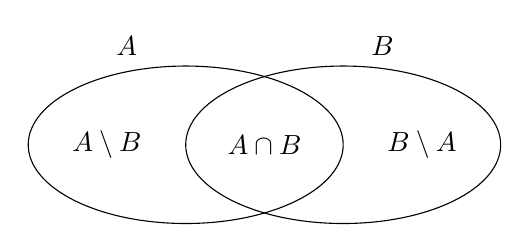
\begin{tikzpicture}[scale=0.5]
\draw (-3.5,1.5) ellipse (4 and 2);
\draw (0.5,1.5) ellipse (4 and 2);
\node at (-5.5,1.5) {$A\setminus B$};
\node at (-1.5,1.5) {$A\cap B$};
\node at (2.5,1.5) {$B\setminus A$};
\node at (-5,4) {$A$};
\node at (1.5,4) {$B$};
\end{tikzpicture}
\end{center}
By writing $A = (A\setminus B ) \cup (A\cap B)$ and $B = (B\setminus A ) \cup (A\cap B)$ and using the additivity and positivity of $\mu$, we have
\bi{rCl}
\mu(A)+\mu(B)& = &\mu((A\setminus B ) \cup (A\cap B))+\mu((B\setminus A ) \cup (A\cap B))\\
& = &\mu(A\setminus B ) + 2\mu(A\cap B)+\mu(B\setminus A )\\
& = &\mu(A\cup B ) + \mu(A\cap B)\\
& \geq & \mu(A\cup B ).
\ei
\item We now extend this to finite unions by induction. Let $\{A_n\}_{n\in\N}$ be a sequence in $\Sigma$ and suppose that
\bse
\mu\biggl(\bigcup_{\,i=0}^{n}A_i\biggr)\leq \sum_{i=0}^{n}\mu(A_i)
\ese
for some $n\in \N$. Then, by part (a), we have
\bi{rCl}
\mu\biggl(\bigcup_{\,i=0}^{\,n+1}A_i\biggr) & = & \mu\biggl(A_{n+1}\cup\bigcup_{i=0}^{n}A_i\biggr)\\
& \leq &\mu (A_{n+1})+\mu\biggl(\bigcup_{\,i=0}^{n}A_i\biggr)\\
& \leq &\mu (A_{n+1})+\sum_{i=0}^{n}\mu(A_i)\\
& = & \sum_{i=0}^{n+1}\mu(A_i).
\ei
Hence, by induction on $n$ with base case $n=1$ and noting that the case $n=0$ is trivial (it reduces to $\mu(A_0)=\mu(A_0)$), we have
\bse
\forall \, n \in \N : \ \mu\biggl(\bigcup_{\,i=0}^{n}A_i\biggr)\leq \sum_{i=0}^{n}\mu(A_i).
\ese
\item Let $\{A_n\}_{n\in\N}$ be a sequence in $\Sigma$. Define $B_n:=\bigcup_{i=0}^nA_n$. Then, $\{B_n\}_{n\in\N}$ is an increasing sequence in $\Sigma$. Hence, by continuity from above of $\mu$, we have
\bi{rCl}
\mu\biggl(\bigcup_{\,n=0}^{\infty}A_n\biggr) &=& \mu\biggl(\bigcup_{\,n=0}^{\infty}B_n\biggr)\\
& = & \lim_{n\to\infty}\mu(B_n)\\
& = & \lim_{n\to\infty}\mu\biggl(\bigcup_{\,i=0}^{n}A_i\biggr)\\
& \leq & \lim_{n\to\infty}\sum_{i=0}^n\mu(A_i)\\
& = & \sum_{i=0}^\infty\mu(A_i)
\ei
which is what we wanted. \qedhere
\een
\eq

\bd
Let $(M,\Sigma,\mu)$ be a measure space. The measure $\mu$ is said to be \emph{finite}\index{finite measure} if there exists a sequence $\{A_n\}_{n\in\N}$ in $\Sigma$ such that $\bigcup_{n=0}^{\infty}A_n=M$ and
\bse
\forall \, n \in \N : \ \mu(A_n)<\infty.
\ese
\ed

\be
The counting measure on $(\N,\mathscr{P}(\N))$ is finite. To see this, define $A_n:=\{n\}$. Then, clearly $\bigcup_{n=0}^{\infty}A_n=\N$ and $\mu(A_n)=|\{n\}|=1<\infty$ for all $n\in \N$.
\ee



\subsection[\texorpdfstring{Borel $\sigma$-algebras}{Borel \textsigma-algebras}]{Borel $\sigma$-algebras}

We have already remarked the parallel between topologies and $\sigma$-algebras. A further similarity stems from the fact that, just like for topologies, interesting $\sigma$-algebras are hardly ever given explicitly, except in some simple cases. In general, they are defined implicitly by some membership condition.

\bp
Let $M$ be a set and let $\{ \Sigma_i : i \in I\}$ be a collection of $\s$-algebras on $M$. Define the set
\bse
\Sigma :=\bigcap_{i\in I}\Sigma_i = \{ A \in \mathscr{P}(M) \mid A \in \Sigma_i, \forall \, i \in I \}.
\ese
Then, $\Sigma$ is a $\s$-algebra on $M$.
\ep
\bq
We simply check that $\Sigma$ satisfies the defining properties of a $\sigma$-algebra.
\ben[label=(\roman*)]
\item We have $M \in \Sigma_i$ for all $i \in I$ and hence $ M \in \Sigma$.  
\item Let $A \in \Sigma$. Then, $A \in \Sigma_i$ for all $i \in I$
and, since each $\Sigma_i$ is a $\s$-algebra, we also have $M\setminus A \in \Sigma_i$ for all $i\in I$. Hence, $M\setminus A \in \Sigma$.
\item Let $\{A_n\}_{n\in\N}$ be a sequence in $\Sigma$. Then, $\{A_n\}_{n\in\N}$ is a sequence in each $\Sigma_i$. Thus,
\bse
\forall \, i\in I : \ \bigcup_{n=0}^{\infty}{A_n} \in \Sigma_i.
\ese
Hence, we also have $\bigcup_{n=0}^{\infty}{A_n} \in \Sigma$. \qedhere
\een
\eq

\bd
Let $M$ be a set and let $\mathcal{E}\subseteq\mathscr{P}(M)$ be a collection of subsets of $M$. The $\sigma$-algebra \emph{generated} by $\mathcal{E}$, denoted $\sigma(\mathcal{E})$, is the smallest $\sigma$-algebra on $M$ containing all the sets in $\mathcal{E}$. That is,
\bse
A\in\sigma(\mathcal{E}) \quad \Leftrightarrow \quad  \text{for all $\sigma$-algebras }\Sigma \text{ on } M :\ \mathcal{E}\subseteq \Sigma \, \Rightarrow\, A\in \Sigma
\ese
or, by letting $\{\Sigma_i\mid i\in I\}$ be the collection of $\sigma$-algebras on $M$ such that $\mathcal{E}\subseteq \Sigma$,
\bse
\sigma(\mathcal{E}):=\bigcap_{i\in I}\Sigma_i.
\ese
\ed
The set $\mathcal{E}$ is called a \emph{generating set} for $\sigma(\mathcal{E})$. Observe that the second characterisation makes it manifest that $\sigma(\mathcal{E})$ is indeed a $\sigma$-algebra on $M$ by the previous proposition.

\bt
Let $(M,\Sigma)$ be a measurable space. Then, $\Sigma=\sigma(\mathcal{E})$ for some $\mathcal{E}\subseteq\mathscr{P}(M)$.
\et

%That is, every $\sigma$-algebra on $M$ is generated by some collection of subsets of $M$. 
This generating construction immediately allows us to link the notions of topology and $\sigma$-algebra on a set $M$ via the following definition.

\bd
Let $(M,\mathcal{O})$ be a topological space. The \emph{Borel $\sigma$-algebra}\index{Borel $\sigma$-algebra} on $(M,\mathcal{O})$ is $\sigma(\mathcal{O})$. 
\ed

Recall that a topology on $M$ is a collection $\mathcal{O}\subseteq\mathscr{P}(M)$ of subsets of $M$ which contains $\varnothing$ and $M$ and is closed under finite intersections and arbitrary (even uncountable) unions. The elements of the topology are called \emph{open sets}.
Of course, while there many choices of $\sigma$-algebra on $M$, if we already have a topology $\mathcal{O}$ on $M$, then the associated Borel $\sigma$-algebra is very convenient choice of $\sigma$-algebra since, as we will soon see, it induces a measurable structure which is ``compatible'' with the already given topological structure.

This is, in fact, the usual philosophy in mathematics: we always let the stronger structures induce the weaker ones, unless otherwise specified. For instance, once we have chosen an inner product on a space, we take the norm to be the induced norm, which induces a metric, which in turn induces a topology on that space, from which we now know how to obtain a canonical $\sigma$-algebra. 

We remark that, while the Borel $\sigma$-algebra on a topological space is generated by the open sets, in general, it contains much more that just the open sets.

\be
Recall that the standard topology on $\R$, denoted $\mathcal{O}_{\R}$, is defined by
\bse
A\in \mathcal{O}_{\R} \quad \Leftrightarrow \quad \forall \, a\in A : \exists \, \varepsilon > 0 : \forall \, r \in \R : \ |r-a|<\varepsilon \, \Rightarrow\,  r\in A.
\ese
In fact, the elements of $\mathcal{O}_{\R}$ are at most countable unions of open intervals in $\R$. Consider now the Borel $\sigma$-algebra on $(\R,\mathcal{O}_{\R})$. Let $a<b$. Then, for any $n\in \N$, the interval $(a-\tfrac{1}{n},b)$ is open. Hence, $\{(a-\tfrac{1}{n},b)\}_{n\in \N}$ is a sequence in $\sigma(\mathcal{O}_{\R})$. Since $\sigma$-algebras are closed under countable intersections, we have
\bse
\bigcap_{n=0}^{\infty}(a-\tfrac{1}{n},b) = [a,b) \in \sigma(\mathcal{O}_{\R}).
\ese
Hence, $\sigma(\mathcal{O}_{\R})$ contains, in addition to all open intervals, also all half-open intervals. It is not difficult to show that it contains all closed intervals as well. In particular, since singletons are closed, $\sigma(\mathcal{O}_{\R})$ also contains all countable subsets of $\R$. In fact, it is non-trivial\footnoteurl{https://en.wikipedia.org/wiki/Borel_set#Non-Borel_sets}{} to produce a subset of $\R$ which is not contained in $\sigma(\mathcal{O}_{\R})$.
\ee

\subsection[\texorpdfstring{Lebesgue measure on $\R^d$}{Lebesgue measure on R\textasciicircum d}]{Lebesgue measure on $\R^d$}

\bd
Let $(M,\Sigma,\mu)$ be a measure space. If $A\in\Sigma$ is such that $\mu(A)=0$, then $A$ is called a \emph{null set}\index{null set} or a \emph{set of measure zero}. 
\ed

The following definition is not needed for the construction of the Lebesgue measure. However, since it is closely connected with that of null set and will be used a lot in the future, we chose to present it here.

\bd
Let $(M,\Sigma,\mu)$ be a measure space and let $P$ be some property or statement. We say that $P$ holds \emph{almost everywhere}\index{almost everywhere} on $M$ if
\bse
\exists \, Z\in \Sigma : \ \mu(Z) = 0 \, \text{ and } \, \forall \, m\in M\setminus Z : \, P(m).
\ese
\ed
In other words, the property $P$ is said to hold almost everywhere on $M$ if it holds everywhere on $M$ except for a null subset of $M$.
\be
Let $(M,\Sigma,\mu)$ be a measure space and let $f,g\cl M\to N$ be maps. We say that $f$ and $g$ are \emph{almost everywhere equal}, and we write $f=_{\mathrm{a.e.}}g$, if there exists a null set $Z\in \Sigma$ such that
\bse
\forall \, m\in M\setminus Z : \ f(m)=g(m).
\ese
The case $f=g$ corresponds to $Z=\varnothing$.
\ee

\bd
A measure $\mu\cl \Sigma\to [0,\infty]$ is said to be \emph{complete} if every subset of every null set is measurable, i.e.\
\bse
\forall \, A\in \Sigma :\forall \, B\in\mathscr{P}(A) : \ \mu(A)=0 \,\Rightarrow \, B\in\Sigma.
\ese
\ed
Note that since for any $A,B\in\Sigma$, $B\subseteq A$ implies $\mu(B)\leq\mu(A)$, it follows that every subset of a null set, if measurable, must also be a null set.

\bd
Let $(M,\Sigma,\mu)$ be a measure space and let $(M,+,\cdot)$ be a vector space. The measure $\mu$ is said to be \emph{translation-invariant} if
\bse
\forall \, m\in M : \forall \, A\in \Sigma : \quad A+m\in\Sigma\ \text{ and }\ \mu(A+m)=\mu(A),
\ese
where $A+m := \{a+m\mid a\in A\}$.
\ed

\bt
Let $\mathcal{O}_{\R^d}$ be the standard topology on $\R^d$. There exists a unique complete, translation-invariant measure 
\bse
\lambda^d\cl\sigma(\mathcal{O}_{\R^d})\to[0,\infty]
\ese
such that for all $a_i,b_i\in\R$ with $1\leq i\leq d$ and $a_i<b_i$, we have
\bse
\lambda^d\bigl([a_1,b_1)\times\cdots\times[a_d,b_d)\bigr) = \prod_{i=1}^d(b_i-a_i).
\ese
\et

\bd
The measure $\lambda^d$ is called the \emph{Lebesgue measure} on $\R^d$.
\ed

The superscript $d$ in $\lambda^d$ may be suppressed if there is no risk of confusion. Note that the Lebesgue measure on $\R$, $\R^2$ and $\R^3$ coincides with the standard notions of length, area and volume, with the further insight that these are only defined for the elements of the respective Borel $\sigma$-algebras.

\bp
The Lebesgue measure on $\R$ is finite.
\ep
\bq
Consider the sequence $\{[a_n,a_n+1)\}_{n\in\N}$ where
\bse
a_n = %\tfrac{1}{4} (-1)^n (2 n-1 + (-1)^n )
\begin{cases}
-\tfrac{1}{2}n & \text{ if $n$ is even}\\
\tfrac{1}{2}(n+1) & \text{ if $n$ is odd}.
\end{cases}
\ese
That is, $\{a_n\}_{n\in\N}$ is the sequence $(0,1,-1,2,-2,3,-3,\ldots)$.\\


\begin{center}
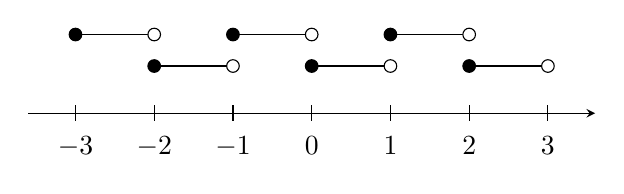
\begin{tikzpicture}
\foreach \i in {-3,-2,-1,0,1,2,3} {
\draw (\i,0.1)--(\i,-0.1) node[below=2pt] {$\i$};
};
\foreach \i in {-3,-1,1} {
 \foreach \j in {0,1} {
  \draw (\i+\j,1-0.4*\j)--(\i+\j+1,1-0.4*\j) ;
  \draw[fill] (\i+\j,1-0.4*\j) circle [radius=0.08] ;
  \draw[fill=white] (\i+\j+1,1-0.4*\j) circle [radius=0.08] ;
};};
\draw[->]  (-3.6,0)--(3.6,0);
\end{tikzpicture}
\end{center}
Clearly, we have $\bigcup_{n=0}^{\infty}[a_n,a_n+1) = \R$. Since, for all $n\in \N$, $[a_n,a_n+1)\in\sigma(\mathcal{O}_{\R})$ and $\lambda\bigl([a_n,a_n+1)\bigr) = 1<\infty$, the Lebesgue measure $\lambda$ is finite.
\eq

This can easily be generalised to show that $\lambda^d$ is finite for all $d\geq 1$.


\subsection{Measurable maps}

As we have remarked earlier, once we introduce a new structure, we should immediately think about the associated structure-preserving maps. In the case of measurable spaces, a measurable map is one that preserves the ``measurability'' structure.

\bd
Let $(M,\Sigma_M)$ and $(N,\Sigma_N)$ be measurable spaces. A map $f\cl M\to N$ is said to be \emph{measurable}\index{measurable map} if
\bse
\forall \, A\in \Sigma_N : \ \preim_f(A)\in \Sigma_M.
\ese
\ed

Note that this is exactly the definition of continuous map between topological spaces, with ``continuous'' replaced by ``measurable'' and topologies replaced by $\sigma$-algebras. 

\bl
Let $(M,\Sigma_M)$ and $(N,\Sigma_N)$ be measurable spaces. A map $f\cl M\to N$ is measurable if, and only if,
\bse
\forall \, A\in \mathcal{E} : \ \preim_f(A)\in \Sigma_M,
\ese
where $\mathcal{E}\subseteq\mathscr{P}(N)$ is a generating set of $\Sigma_N$.
\el

\bc
Let $(M,\mathcal{O}_M)$ and $(N,\mathcal{O}_N)$ be topological spaces. Any continuous map $M\to N$ is measurable with respect to the Borel $\sigma$-algebras on $M$ and $N$.
\ec

Recall that a map $\R\to\R$ is monotonic if it is either increasing or decreasing.

\bc
Any monotonic map $\R\to\R$ is measurable with respect to the Borel $\sigma$-algebra (with respect to $\mathcal{O}_{\R}$).
\ec

\bp
Let $(M,\Sigma_M)$, $(N,\Sigma_N)$ and $(P,\Sigma_P)$ be measurable spaces. If $f\cl M\to N$ and $g\cl N\to P$ are both measurable, the so is their composition $g \circ f\cl M\to P$.
\ep

\bq
Let $A\in \Sigma_P$. As $g$ is measurable, we have $\preim_g(A)\in\Sigma_N$. Then, since $f$ is measurable, it follows that
\bse
\preim_f(\preim_g(A)) = \preim_{g\circ f}(A) \in \Sigma_M.
\ese
Hence, $g\circ f$ is measurable.
\eq

\bp
Let $(M,\Sigma_M)$ and $(N,\Sigma_N)$ be measurable spaces and let $\{f_n\}_{n\in\N}$ be a sequence of measurable maps from $M$ to $N$ whose pointwise limit is $f$. Then, $f$ is measurable.
\ep
Recall that $\{f_n\}_{n\in\N}$ converges pointwise to $f\cl M\to N$ if
\bse
\forall \, m\in M : \ \lim_{n\to \infty}f_n(m)=f(m).
\ese
This is in contrast with continuity, as pointwise convergence of a sequence of continuous maps is not a sufficient condition for the continuity of the pointwise limit. In the case of real or complex-valued maps, a sufficient condition is convergence with respect to the supremum norm. 

\subsection{Push-forward of a measure}

If we have a structure-preserving map $f$ between two instances $A$ and $B$ of some structure, and an object on $A$ (which depends in some way on the structure), we can often use $f$ to induce a similar object on $B$. This is generically called the push-forward of that object along the map $f$.

\bp
Let $(M,\Sigma_M,\mu)$ be a measure space, let $(N,\Sigma_N)$ be a measurable space and let $f\cl M\to N$ be a measurable map. Then, the map
\bi{rrCl}
f_*\mu\cl & \Sigma_N & \to & [0,\infty]\\
& A & \mapsto & \mu(\preim_f(A))
\ei
is a measure on $(N,\Sigma_N)$ called the \emph{push-forward}\index{push-forward of a measure} of $\mu$ along $f$.
\ep

That $f_*\mu$ is a measure follows easily from the fact that $\mu$ is a measure and basic properties of pre-images of maps, namely
\bi{rCl}
\preim_f(A\setminus B) & = & \preim_f(A)\setminus \preim_f(B)\\ \preim_f\biggl(\bigcup_{\,i\in I}A_i\biggr) & = & \bigcup_{i\in I}\preim_f(A_i).
\ei












\newpage

\section{Integration of measurable functions}

We will now focus on measurable functions $M\to \overline{\R}$ and define their integral on a subset of $M$ with respect to some measure on $M$, which is called the Lebesgue integral. Note that, even if $M\subseteq\R^d$, the Lebesgue integral of a function need not be with respect to the Lebesgue measure. 

The key application of this material is the definition of the Banach spaces of (classes of) Lebesgue integrable functions $L^p$. The case $p=2$ is especially important since $L^2$ is, in fact, a Hilbert space. It appears a lot in quantum mechanics where it is loosely referred to as the space of square-integrable functions.

\subsection{Characteristic and simple functions}

\bd
Let $M$ be a set and let $A\in\mathscr{P}(M)$. The \emph{characteristic function}\index{characteristic function} of $A$, denoted $\chi_A\cl M\to \R$, is defined by
\bse
\chi_A(m) = \begin{cases}1 & \text{if } m\in A\\ 0& \text{if } m\notin A.\end{cases}
\ese
\ed

\be
Below is the graph of $\chi_{(1,2]}\cl \R \to \R$.
\begin{center}
\begin{tikzpicture}[scale=1.2]
\draw[->] (0,-0.5)--(0,1.75);
\draw[->] (-0.5,0)--(3.5,0);
\foreach \i in {1,2,3}{
\draw (\i,0.08)--(\i,-0.08) node[below=2pt] {$\i$};
};
\draw (0.08,1) -- (-0.08,1) node[left] {$1$};
\draw (0,0) node[below left] {$0$};
\draw (1,1)--(2,1) node[right=3pt] {$\chi_{(1,2]}$};
\draw[dotted] (0,1)--(1,1)--(1,0);
\draw[dotted] (2,1)--(2,0);
\draw[fill=white] (1,1) circle [radius=0.08];
\draw[fill] (2,1) circle [radius=0.08];
\end{tikzpicture}
\end{center}
\ee

The following properties of characteristic functions are immediate.
\bp
\label{prp:characteristic}
Let $M$ be a set and let $A,B\in\mathscr{P}(M)$. Then
\ben[label=(\roman*)]
\item $\chi_{\varnothing}=0$
\item $\chi_{A\cup B} = \chi_A+\chi_B-\chi_{A\cap B}$
\item $\chi_{A\cap B} = \chi_A\chi_B$
\item $\chi_{M\setminus A} + \chi_A = 1$
\een
where the addition and multiplication are pointwise and the $0$ and $1$ in parts (i) and (iv) are the constant functions $M\to \R$ mapping every $m\in M$ to $0\in\R$ and $1\in\R$, respectively.
\ep

\bd
Let $M$ be a set. A function $s\cl M \to \R$ is \emph{simple}\index{simple function} if $s(M) = \{r_1,\ldots,r_n\}$ for some $n\in \N$. 
%Let $(M,\Sigma)$ be a measurable space. A measurable function $s\cl M \to \R$ is said to be \emph{simple}\index{simple function} if $s(M) = \{r_1,\ldots,r_n\}$ for some $n\in \N$. 
\ed
Equivalently, $s\cl M \to \R$ is simple if there exist $r_1,\ldots,r_n\in\R$ and $A_1,\ldots,A_n\in\mathscr{P}(M)$, for some $n\in \N$, such that
\bse
s = \sum_{i=1}^nr_i\chi_{A_i}.
\ese
So $s$ is simple if it is a linear combination of characteristic functions.
% Note that, since $s$ is assumed to be measurable, we have $\preim_s(\{r_i\})\in\Sigma$ for all $1\leq i\leq n$.

\be
Consider the simple function $s\cl \R \to \R$ given by $s:=\chi_{[1,3]}+2\chi_{[2,5]}$.
\begin{center}
\begin{tikzpicture}[scale=1.2]
\draw[->] (0,-0.5)--(0,3.75);
\draw[->] (-0.5,0)--(5.75,0);
\foreach \i in {1,2,3,4,5}{
\draw (\i,0.08)--(\i,-0.08) node[below=2pt] {$\i$};
};
\foreach \i in {1,2,3} {
\draw (0.08,\i) -- (-0.08,\i) node[left] {$\i$};
};
\draw (0,0) node[below left] {$0$};
\draw (1,1)--(2,1);
\draw (2,3)--(3,3);
\draw (3,2)--(5,2);
\draw[dotted] (0,1)--(1,1)--(1,0);
\draw[dotted] (0,3)--(2,3)--(2,0);
\draw[dotted] (0,2)--(3,2);
\draw[dotted] (3,3)--(3,0);
\draw[dotted] (5,2)--(5,0);
\draw[fill] (1,1) circle [radius=0.08];
\draw[fill=white] (2,1) circle [radius=0.08];
\draw[fill] (3,3) circle [radius=0.08];
\draw[fill] (2,3) circle [radius=0.08];
\draw[fill] (5,2) circle [radius=0.08];
\draw[fill=white] (3,2) circle [radius=0.08];
\end{tikzpicture}
\end{center}
By observing the graph, we see that we can re-write $s$ as
\bse
s = \chi_{[1,2)} + 3 \chi_{[2,3]} + 2 \chi_{(3,5]}.
\ese
\ee

\bd
A simple function is said to be in its \emph{standard form} if
\bse
s = \sum_{i=1}^nr_i\chi_{A_i},
\ese
where $A_i \cap A_j = \varnothing$ whenever $i\neq j$.
\ed

Any simple function can be written in standard form. It is clear that if $s$ is in its standard form, then $A_i = \preim_s(\{r_i\})$. 

\bp
Let $(M,\Sigma)$ be a measurable space and let $A,A_1,\ldots,A_n\in\mathscr{P}(M)$. Then
\ben[label=(\roman*)]
\item $\chi_A$ is measurable if, and only if, $A\in\Sigma$
\item if $s=\sum_{i=1}^n r_i \chi_{A_i}$ is a simple function in its standard form, then $s$ is measurable if, and only if, we have $A_i\in \Sigma$ for all $1\leq i\leq n$.
\een
\ep
\subsection{Integration of non-negative measurable simple functions}

We begin with the definition of the integral of a non-negative, measurable, simple function.

\bd
Let $(M,\Sigma,\mu)$ be a measure space and let $s\cl M \to \R$ be a nowhere negative, measurable, simple function whose standard form is $s=\sum_{i=1}^n r_i \chi_{A_i}$. Then, we define
\bse
\int_M \! s \, \d \mu := \sum_{i=1}^nr_i\mu(A_i).
\ese
\ed

Note that the non-negativity condition is essential since $\mu$ takes values in $[0,\infty]$, hence we could have $\mu(A_i)=\infty$ for more that one $A_i$, and if the corresponding coefficients $r_i$ have opposite signs, then we would have $\int_Ms\,\d\mu=\infty-\infty$, which is not defined. For the same reason, we are considering $s\cl M\to [0,\infty)$ rather than $s\cl M\to [0,\infty]$.
\be
Consider the measure space $(\N,\mathscr{P}(\N),\mu)$, where $\mu$ is the counting measure, let $f\cl \N \to \R$ be non-negative and suppose that there exists $N\in\N$ such that $f(n)=0$ for all $n>N$. Then, we can write $f$ as
\bse
f=\sum_{n=0}^Nf(n)\chi_{\{n\}}.
\ese
That is, $f$ is a non-negative, measurable, simple function and therefore
\bse
\int_{\N}\! f \,\d \mu := \sum_{n=0}^Nf(n)\mu(\{n\}) = \sum_{n=0}^Nf(n).
\ese
Hence, the ``integral'' of $f$ over $\N$ with respect to the counting measure is just the sum.
\ee

The need for simple functions to be in their standard form, which was introduced to avoid any potential ambiguity in the definition of their integral, can be relaxed using the following lemma.

\bl
\label{lem:simplelinear}
Let $(M,\Sigma,\mu)$ be a measure space. Let $s$ and $t$ be non-negative, measurable, simple functions $M\to \R$ and let $c\in [0,\infty)$. Then
\bse
\int_M\!(cs+t)\,\d\mu = c\int_M\!s\,\d\mu+\int_M\!t\,\d\mu
\ese
\el

\bp
Let $(M,\Sigma,\mu)$ be a measure space and let $s=\sum_{i=1}^n r_i \chi_{A_i}$ be a non-negative, measurable, simple function $M\to \R$ not necessarily in its standard form. Then
\bse
\int_M\!s\,\d\mu = \sum_{i=1}^nr_i\mu(A_i).
\ese
\ep

\bc
Let $(M,\Sigma,\mu)$ be a measure space. Let $s$ and $t$ be non-negative, measurable, simple functions $M\to \R$ such that $s\leq t$ (that is, $s(m)\leq t(m)$ for all $m\in M$). Then
\bse
\int_M\!s\,\d\mu \leq \int_M\!t\,\d\mu. 
\ese
\ec

\bl
Let $(M,\Sigma, \mu)$ be a measure space and let $s = \sum_{i=1}^n{r_i\chi_{A_i}}$ be a non-negative, measurable, simple function $M\to\R$. Define the map
\bi{rrCl}
\nu_s \cl & \Sigma & \to & [0,\infty]\\
& A & \mapsto &  \int_M \! s\chi_A \, \d \mu,
\ei
where $s\chi_A$ is the pointwise product of $s$ and $\chi_A$. Then, $\nu_s$ is a measure on $(M,\Sigma)$.
\el

\bq
First, note that we have
\bse
\int_M \! s\chi_A \, \d \mu = \int_M \biggl(\sum_{\,i=1}^nr_i\chi_{A_i}\chi_{A}\biggr) \d \mu = \int_M \biggl(\sum_{\,i=1}^nr_i\chi_{A_i\cap A}\biggr) \d \mu  =\sum_{i=1}^nr_i\mu({A_i\cap A)}.
\ese
We now check that $\nu$ satisfies the defining properties of a measure.
\ben[label=(\roman*)]
\item $\displaystyle\nu_s(\varnothing):= \int_M \! s\chi_{\varnothing} \, \d \mu = \sum_{i=1}^n{r_i\mu({A_i\cap \varnothing})} = \sum_{i=1}^n{r_i\mu(\varnothing)} = 0$
\item Let $\{B_j\}_{j\in\N}$ be a pairwise disjoint sequence in $\Sigma$. Then
\bi{rCl}
\nu_s \biggl( \bigcup_{\,j=0}^{\infty}B_j \biggr) &=& \int_M \! s\chi_{ \left( \bigcup_{j=0}^{\infty}B_j \right)} \, \d \mu \\
& = & \sum_{i=1}^n r_i  \mu \biggl( \bigcup_{\,j=0}^{\infty}(A_i \cap B_j )\biggr)\\
&=& \sum_{j=0}^{\infty}\sum_{i=1}^n r_i \mu (A_i \cap B_j )\\
&=& \sum_{j=0}^{\infty}\int_M \! s\chi_{B_j} \, \d \mu \\
&=& \sum_{j=0}^{\infty}\nu_s(B_j) .
\ei
\een
Thus, $\nu_s$ is a measure on $(M,\Sigma)$. \qedhere
\eq

\subsection{Integration of non-negative measurable functions}

As we are interested in measurable functions $M\to\overline{\R}$, we need to define a $\sigma$-algebra on $\overline{\R}$. We cannot use the Borel $\sigma$-algebra since we haven't even defined a topology on $\overline{\R}$. In fact, we can easily get a $\sigma$-algebra on $\overline{\R}$ as follows.

\bp
The set $\overline{\Sigma}:=\{A\in \mathscr{P}(\overline{\R})\mid A\cap \R \in \sigma(\mathcal{O}_{\R})\}$ is a $\sigma$-algebra on $\overline{\R}$.
\ep
In other words, we can simply ignore the infinities in a subset of $\overline{\R}$ and consider it to be measurable if $A\setminus\{-\infty,+\infty\}$ is in the Borel $\sigma$-algebra of $\R$. We will always consider $\overline{\R}$ to be equipped with this $\sigma$-algebra.

\bl
\label{lem:measurable}
Let $(M,\Sigma)$ be a measurable space and let $f,g\cl M\to \overline{\R}$ be measurable. Then, the following functions are measurable.
\ben[label=(\roman*)]
\item $cf+g$, for any $c\in \R$
\item $|f|$ and $f^2$
\item $fg$ (pointwise product) if $f$ and $g$ are nowhere infinite
\item $\max(f,g)$ (defined pointwise).
\een
\el


\bd
Let $(M,\Sigma,\mu)$ be a measure space and let $f\cl M\to\overline{\R}$ be a non-negative, measurable function. Denote by $S$ the set of all non-negative, measurable, simple functions $s\cl M \to \R$ such that $s\leq f$. Then, we define
\bse
\int_M\! f\, \d \mu := \sup_{s\in S} \int_M\! s\, \d \mu.
\ese
\ed

\br
It is often very convenient to introduce the notation
\bse
\int_M\!f(x)\,\mu(\d x) \equiv \int_M\! f\, \d \mu,
\ese
where $x$ is a dummy variable and could be replaced by any other symbol. The reason why this is a convenient notation is that, while some functions have standard symbols but cannot be easily represented by an algebraic expression (e.g. characteristic functions), others are easily expressed in terms of an algebraic formula but do not have a standard name. For instance, it is much easier to just write
\bse
\int_{\R}  x^2\,\mu(\d x)
\ese
than having to first denote the function $\R\to\R$, $x\mapsto x^2$ by a generic $f$ or, say, the more specific $\mathrm{sq}_{\R}$, and then write 
\bse
\int_\R\mathrm{sq}_{\R}\, \d \mu.
\ese
In computer programming, this is akin to defining \emph{anonymous functions}.
\er

\bd
Let $(M,\Sigma,\mu)$ be a measure space and let $f\cl M\to\overline{\R}$ be a non-negative, measurable function. For any $A\in \Sigma$ (that is, any measurable subset of $M$), we define
\bse
\int_A\! f\, \d \mu := \int_M\! f\chi_A\, \d \mu.
\ese
\ed
Note that the product $f\chi_A$ is measurable by part (iii) of \Cref{lem:measurable}.

\bl
\label{lem:intineq}
Let $(M,\Sigma,\mu)$ be a measure space, let $f,g\cl M\to\overline{\R}$ be non-negative, measurable functions such that $f\leq g$, and let $A,B\in \Sigma$ be such that $A\subseteq B$. Then
\ben[label=(\roman*)]
\item $\displaystyle \int_M\! f\, \d \mu \leq \int_M\! g\, \d \mu$
\item $\displaystyle \int_A\! f\, \d \mu \leq \int_B\! f\, \d \mu$.
\een
\el

\bq
\ben[label=(\roman*)]
\item Denote by $S_f$ and $S_g$ the sets of non-negative, measurable, simple functions that are less than or equal to $f$ and $g$, respectively. As $f\leq g$, we have $S_f\subseteq S_g$ and hence
\bse
\int_M\! f\, \d \mu :=  \sup_{s\in S_f}\, \int_M\! s\, \d \mu \leq \sup_{s\in S_g}\, \int_M\! s\, \d \mu =: \int_M\! g\, \d \mu.
\ese
\item Since $A\subseteq B$, for any $m\in M$ we have
\bse
f(m)\chi_A(m) \leq f(m)\chi_B(m).
\ese
In fact, we have equality whenever $m\in A$ or $m\in M\setminus B$, while for $m\in B\setminus A$ the left hand side is zero and the right-hand side is non-negative. Hence, $f\chi_A\leq f\chi_B$ and thus, by part (i), we have
\bse
\int_A\! f\, \d \mu := \int_M\! f\chi_A\, \d \mu \leq\int_M\! f\chi_B\, \d \mu =: \int_B\! f\, \d \mu \qedhere
\ese
\een
\eq

\bp[Markov inequality]
Let $(M,\Sigma,\mu)$ be a measure space and let $f\cl M\to\overline{\R}$ be a non-negative, measurable function. For any $z\in [0,\infty]$, we have
\bse
\int_M\! f\, \d \mu \geq z\, \mu(\preim_f([z,\infty])).
\ese
\ep

Equality is achieved whenever $z$ is an upper bound for $f$.

\begin{center}
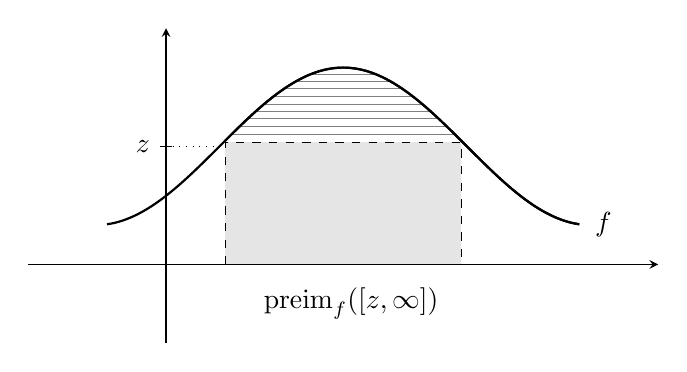
\begin{tikzpicture}
\foreach \i in {0.25,0.6,0.95,1.3,1.65,2.05,2.5,3,3.55} {
\draw[gray] (-0.5+0.3*\i,{1.5+cos deg (-0.5+0.3*\i-1)}) -- (2.5-0.3*\i,{1.5+cos deg (2.5-0.3*\i-1)}) ;
};
\fill[lightergray] (-0.5,0) rectangle (2.5,1.55);
\draw[dashed,thin] (-0.5,0)--(-0.5,1.55)--(2.5,1.55)--(2.5,0);
\draw (-1.17,1.5)--(-1.33,1.5) node[left] {$z$};
\draw (1.1,-0.5) node {$\preim_f([z,\infty])$};
\draw[dotted] (-1.25,1.5)--(-0.5,1.5);
\draw [thick,smooth,samples=100,variable=\x,domain=-2:4] plot(\x,{1.5+cos deg (\x-1)}) node[right=2pt] {$f$};
\draw [thick,smooth,samples=100,variable=\x,domain=-0.5:4] plot(\x,{1.5+cos deg (\x-1)});
\draw[->,thin] (-3,0)--(5,0);
\draw[->,thin] (-1.25,-1)--(-1.25,3);
\end{tikzpicture}
\end{center}

The following is the pivotal theorem of Lebesgue integration.

\bt[Monotone convergence theorem]
Let $(M,\Sigma,\mu)$ be a measure space and let $\{f_n\}_{n\in\N}$ be a sequence of non-negative, measurable functions $M\to\overline{\R}$ such that $f_{n+1}\geq f_n$ for all $n\in \N$. If there exists a function $f\cl M\to \overline{\R}$ such that
\bse
\forall \, m \in M : \ \lim_{n\to\infty}f_n(m) = f(m)
\ese
(i.e. $f$ is the pointwise limit of  $\{f_n\}_{n\in\N}$), then $f$ is measurable and
\bse
\lim_{n\to\infty}\int_M\! f_n \, \d \mu = \int_M\! f \, \d \mu.
\ese
\et

\br
Observe that this result is in stark contrast with what one may be used from Riemann integration, where pointwise converge of a sequence of integrable functions $\{f_n\}_{n\in\N}$ is \emph{not} a sufficient condition for the integral of the limit $f$ to be equal to the limit of the integrals of $f_n$ or, in fact, even for $f$ to be integrable. For these, we need stronger conditions on the sequence $\{f_n\}_{n\in\N}$, such as uniform converge.
\er

The definition of the integral as a supremum is clear and geometrically reasonable. However, it is in general very difficult to evaluate
the integral of any particular function using it. The monotone convergence theorem provides a much simpler way to evaluate the integral. One can show that, for any non-negative, measurable function $f$, there exists an increasing sequence $\{s_n\}_{n\in\N}$ of non-negative, measurable, simple functions (which can be explicitly constructed from $f$) whose pointwise limit is $f$, and hence we have
\bse
\int_M\! f \, \d \mu = \lim_{n\to\infty}\int_M\! s_n \, \d \mu,
\ese
where the right-hand side can usually be evaluated fairly easily.

\be
Consider the measure space $(\N,\mathscr{P}(\N),\mu)$, where $\mu$ is the counting measure, and let $f\cl \N \to \overline{\R}$ be non-negative. Note that the choice of $\sigma$-algebra $\mathscr{P}(\N)$ on $\N$ makes every function on $\N$ (to any measurable space) measurable. Define, for every $n\in \N$,  
\bse
s_n=\sum_{i=0}^nf(i)\chi_{\{i\}}.
\ese
Then, $\{s_n\}_{n\in\N}$ is an increasing sequence of non-negative, measurable, simple functions whose pointwise limit is $f$ and therefore, by the monotone convergence theorem,
\bse
\int_{\N}\! f \,\d \mu =\lim_{n\to\infty}\int_{\N}\! s_n \, \d \mu = \lim_{n\to\infty}\sum_{i=0}^nf(i)\mu(\{i\}) = \sum_{i=0}^{\infty}f(i).
\ese
If you every wondered why series seem to share so many properties with integrals, the reason is that series are just integrals with respect to a discrete measure.
\ee

The monotone convergence theorem can be used to extend some of properties of integrals of non-negative, measurable simple functions to non-negative, measurable functions which are not-necessarily simple.

\bl
Let $(M,\Sigma,\mu)$ be a measure space, let $f,g\cl M\to \overline{\R}$ be non-negative, measurable functions and let $c\in [0,\infty)$. Then
\ben[label=(\roman*)]
\item $\displaystyle \int_{M}\! (cf+g) \,\d \mu = c\int_{M}\! f \,\d \mu +\int_{M}\! g \,\d \mu $
\item the map $\nu_f\cl \Sigma\to [0,\infty]$ defined by $\displaystyle \nu_f(A):=\int_A\, f\, \d \mu$ is a measure on $(M,\Sigma)$
\item for any $A\in\Sigma$, we have $\displaystyle \int_{M}\!f \,\d \mu =  \int_{A}\!f \,\d \mu+ \int_{M\setminus A}\!f \,\d \mu$.
\een
\el

\bq
\ben[label=(\roman*)]
\item Let $\{s_n\}_{n\in\N}$ and $\{t_n\}_{n\in\N}$ be increasing sequences of non-negative, measurable, simple functions whose pointwise limits are $f$ and $g$, respectively. Then, it is easy to see that $\{cs_n+t_n\}_{n\in\N}$ is an increasing sequence of non-negative, measurable, simple functions whose pointwise limit is $cf+g$. Hence, by \Cref{lem:simplelinear} and the monotone converge theorem
\bi{rCl}
\int_M\! (cf+g) \,\d \mu & = &  \lim_{n\to\infty}\int_M\! (cs_n+t_n) \, \d \mu\\
& = &  \lim_{n\to\infty}\biggl(c\int_M\! s_n \, \d \mu+\int_M\! t_n \, \d \mu\biggr)\\
& = &  c\lim_{n\to\infty}\int_M\! s_n \, \d \mu+\lim_{n\to\infty}\int_M\! t_n \, \d \mu\\
& = &  c\int_{M}\! f \,\d \mu +\int_{M}\! g \,\d \mu.
\ei
\item To check that $\nu_f$ is a measure on $(M,\Sigma)$, first note that we have
\bse
\nu_f(\varnothing) = \int_{\varnothing}\! f\, \d \mu :=\int_{M}\! f\chi_{\varnothing}\, \d \mu = 0.
\ese
Let $\{A_i\}_{i\in\N}$ be a pairwise disjoint sequence in $\Sigma$. Define, for any $n\in \N$,
\bse
f_n:=f\chi_{\left(\bigcup_{i=0}^nA_i\right)}.
\ese
Since, for all $n\in \N$, we have $\bigcup_{i=0}^{n}A_i\subseteq\bigcup_{i=0}^{n+1}A_i$ and $f$ is non-negative, $\{f_n\}_{n\in\N}$ is an increasing sequence of non-negative, measurable, simple functions whose pointwise limits is $f\chi_{\left(\bigcup_{i=0}^{\infty}A_i\right)}$. Hence, by recalling \Cref{prp:characteristic}, we have
\bi{rCl}
\nu_f\biggl(\bigcup_{\,i=0}^{\infty}A_i\biggr) & := & \int_{\,\bigcup_{i=0}^{\infty}A_i}\! f \, \d \mu\\
& = & \int_{M} \!f\chi_{\left(\bigcup_{i=0}^{\infty}A_i\right)} \, \d \mu\\
& = & \lim_{n\to\infty}\int_{M} \!f\chi_{\left(\bigcup_{i=0}^{n}A_i\right)} \, \d \mu\\
& = & \lim_{n\to\infty}\int_{M} \biggl(f\sum_{i=0}^{n}\chi_{A_i}\biggr) \, \d \mu\\
& = & \lim_{n\to\infty}\biggl(\sum_{\,i=0}^{n}\int_{M}\! f\chi_{A_i}\, \d \mu\biggr) \\
& = & \sum_{i=0}^{\infty}\nu_f(A_i) .
\ei
\item Note that $A\cap (M\setminus A)=\varnothing$. Hence, by using the fact that $\nu_f$ from part (ii) is a measure on $(M,\Sigma)$, we have
\bse
\int_M\! f \, \d \mu  =  \nu_f(M) =  \nu_f(A)+\nu_f(M\setminus A) =  \int_A\! f\, \d \mu + \int_{M\setminus A}\! f\, \d \mu. \qedhere
\ese
\een
\eq

Part (i) of the previous lemma and the monotone convergence theorem also imply that, for any sequence $\{f_n\}_{n\in\N}$ of non-negative, measurable functions, we have
\bse
\int_M \biggl(\sum_{\,n=0}^{\infty}f_n \biggr) \d \mu = 
\sum_{n=0}^{\infty} \int_M \! f_n \, \d \mu.
\ese
Again, note that this result does \emph{not} hold for the Riemann integral unless stronger conditions are places on the sequence $\{f_n\}_{n\in\N}$.

Finally, we have a simple but crucial result for Lebesgue integration.

\bt
\label{thm:aezero}
Let $(M,\Sigma,\mu)$ be a measure space and let $f\cl M\to\overline{\R}$ be a non-negative, measurable function. Then
\bse
\int_M\! f\, \d \mu = 0 \quad \Leftrightarrow \quad f=_{\mathrm{a.e.}} 0.
\ese
\et

\bq
\begin{itemize}
\item[$(\Rightarrow)$] Suppose that $\int_Mf\,\d\mu=0$. Define $A_n:=\{m\in M \mid f(m)>\tfrac{1}{n+1}\}$ and let
\bse
s_n := \tfrac{1}{n+1}\chi_{A_n} .
\ese
By definition of $A_n$, we clearly have $s_n\leq f$ for all $n\in\N$. Hence,
\bse
0\leq \int_M\!s_n\,\d\mu\leq\int_M\!f\,\d\mu=0
\ese
and thus, $\int_Ms_n\,\d\mu=0$ for all $n\in\N$. Since by definition
\bse
\int_M\!s_n\,\d\mu = \tfrac{1}{n+1}\mu(A_n),
\ese
we must also have $\mu(A_n)=0$ for all $n\in\N$. Let $A:=\{m\in M \mid f(m)\neq 0\}$. Then, as $f$ is non-negative, we have
\bse
A = \bigcup_{n=0}^{\infty}A_n=\bigcup_{n=0}^{\infty}\{m\in M \mid f(m)>\tfrac{1}{n+1}\}
\ese
and, since $A_n\subseteq A_{n+1}$ for all $n\in\N$, we have
\bse
\mu(A)=\mu\biggl(\bigcup_{\,n=0}^{\infty}A_n\biggr)=\lim_{n\to\infty}\mu(A_n) = 0.
\ese
Thus, $f$ is zero except on the null set $A$. That is, $f=_{\mathrm{a.e.}}0$. 

\item[$(\Leftarrow)$] Suppose that $f=_{\mathrm{a.e.}}0$. Let $S$ be the set of non-negative, measurable, simple functions $s$ such that $s\leq f$. As $f=_{\mathrm{a.e.}}0$, we have $s=_{\mathrm{a.e.}}0$ for all $s\in S$. Thus, if
\bse
s=\sum_{i=1}^nr_i\chi_{A_i},
\ese
we must have either $r_i=0$ or $\mu(A_i)=0$ for all $1\leq i\leq n$. Hence, for all $s\in S$,
\bse
\int_M\! s \, \d \mu := \sum_{i=1}^nr_i\mu(A_i) =0.
\ese
Therefore, we have
\bse
\int_M\! f \, \d \mu := \sup_{s\in S}\int_M\! s \, \d \mu  = 0.\qedhere
\ese
\end{itemize}
\eq

This means that, for the purposes of Lebesgue integration, null sets can be neglected as they do not change the value of an integral. The following are some examples of this.

\bc
Let $(M,\Sigma,\mu)$ be a measure space, let $A\in\Sigma$ and let $f,g\cl M\to\overline{\R}$ be non-negative, measurable functions. 
\ben[label=(\roman*)]
\item If $\mu(A)=0$, then $\displaystyle\int_A\! f \, \d \mu = 0$
\item If $f=_{\mathrm{a.e.}}g$, then $\displaystyle\int_M\! f \, \d \mu = \int_M\! g \, \d \mu$
\item If $f\leq_{\mathrm{a.e.}}g$, then $\displaystyle\int_M\! f \, \d \mu \leq \int_M\! g \, \d \mu$.
\een
\ec

\bq
\ben[label=(\roman*)]
\item Clearly, $f\chi_A =_{\mathrm{a.e.}}0$ and hence
\bse
\int_A\! f \, \d \mu =\int_M\! f\chi_A  \, \d \mu = 0.
\ese
\item As $f=_{\mathrm{a.e.}}g$, we have $f-g=_{\mathrm{a.e.}}0$ and thus
\bse
0 = \int_M\! (f-g) \, \d \mu =\int_M\! f \, \d \mu-\int_M\! g \, \d \mu.
\ese
\item Let $B:=\{m\in M\mid f(m)>g(m)\}$. As $f\leq_{\mathrm{a.e.}}g$, we have $\mu(B)=0$ and $f\leq g$ on $M\setminus B$. Thus
\bi{C}
\int_M\! f \, \d \mu =\int_B\! f \, \d \mu+\int_{M\setminus B}\! f \, \d \mu
 \leq  \int_{M\setminus B}\! g \, \d \mu \leq \int_M\! g \, \d \mu
\ei
where we used part (i) and \Cref{lem:intineq}. \qedhere
\een
\eq

\be
Consider $(\R,\sigma(\mathcal{O}_{\R}),\lambda)$ and let $f\cl \R \to \R$ be the \emph{Dirichlet function}
\bse
f(r) := \begin{cases}
1 & \text{if } r\in \Q\\
0 & \text{if } r\in \R\setminus \Q.
\end{cases}
\ese
The Dirichlet function is the usual example of a function which is \emph{not} Riemann integrable (on any real interval). We will now show that we can easily assign a numerical value to its integral on any measurable subset of $\R$. First, note that a set $A\in\sigma(\mathcal{O}_{\R})$ is null with respect to the Lebesgue measure if, and only if, 
\bse
\forall \, \varepsilon >0 : \exists \, \{I_n\}_{n\in\N} : \quad A\subset \bigcup_{n=0}^{\infty}I_n \ \text{ and } \ \sum_{n=0}^{\infty}\lambda(I_n)<\varepsilon
\ese
where $\{I_n\}_{n\in\N}$ is a sequence of real intervals. From this, it immediately follows that any countable subset of $\R$ has zero Lebesgue measure. Thus, $\lambda(\Q)=0$ and hence, $f=_{\mathrm{a.e.}}0$. Therefore, by the previous lemmas, we have
\bse
\int_A\! f \, \d \lambda = 0
\ese
for any measurable subset $A$ of $\R$. 
\ee

\subsection{Lebesgue integrable functions}

Since the difference $\infty-\infty$ is not defined, we cannot integrate all measurable functions. There is, however, a very small extra condition (beyond measurability) that determines the class of functions to which we can extend our previous definition.

\bd
Let $(M,\Sigma,\mu)$ be a measure space and let $f\cl M\to\overline{\R}$. The function $f$ is said to be \emph{(Lebesgue) integrable}\index{integrable function} if it is measurable and
\bse
\int_{M}\!|f|\,\d \mu < \infty.
\ese
We denote the set of all integrable functions $M\to\overline{\R}$ by $\mathscr{L}^1_{\R}(M,\Sigma,\mu)$, or simply $\mathscr{L}^1(M)$ if there is no risk of confusion.
\ed

For any $f\cl M\to \overline{\R}$, we define $f^+:=\max(f,0)$ and $f^-:=\max(-f,0)$, which are measurable whenever $f$ is measurable by part (iv) of \Cref{lem:measurable}.

\bse
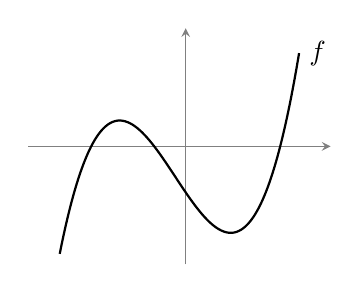
\begin{tikzpicture}[xscale=0.4,yscale=0.5]
\draw[->,thin,gray] (-5,0)--(4.6,0);
\draw[->,thin,gray] (0,-3)--(0,3);
\draw [thick,smooth,samples=100,variable=\x,domain=-4:3.6] plot(\x,{(\x+1)*(\x-3)*(\x+3)*0.13}) node[right] {$f$};
\end{tikzpicture}
\qquad\
\begin{tikzpicture}[xscale=0.4,yscale=0.5]
\draw[->,thin,gray] (-5,0)--(4.6,0);
\draw[->,thin,gray] (0,-3)--(0,3);
\draw [thick,smooth,samples=100,variable=\x,domain=-3:-1] plot(\x,{(\x+1)*(\x-3)*(\x+3)*0.13});
\draw [thick,smooth,samples=100,variable=\x,domain=3:3.6] plot(\x,{(\x+1)*(\x-3)*(\x+3)*0.13}) node[right] {$f^+$};
\draw [thick] (-4,0)--(-3,0);
\draw [thick] (-1,0)--(3,0);
\end{tikzpicture}
\qquad\
\begin{tikzpicture}[xscale=0.4,yscale=0.5]
\draw[->,thin,gray] (-5,0)--(4.6,0);
\draw[->,thin,gray] (0,-3)--(0,3);
\draw [thick,smooth,samples=100,variable=\x,domain=-4:-3] plot(\x,{-(\x+1)*(\x-3)*(\x+3)*0.13});
\draw [thick,smooth,samples=100,variable=\x,domain=-1:3] plot(\x,{-(\x+1)*(\x-3)*(\x+3)*0.13}) node[above=20pt] {$\ f^-$};
\draw [thick] (-3,0)--(-1,0);
\draw [thick] (3,0)--(3.7,0);
\end{tikzpicture}
\ese
Observe that $f=f^+-f^-$ and $|f|=f^++f^-$. Clearly, we have $f^+\leq|f|$ and $f^-\leq |f|$, and hence


\bse
\int_{M}\!|f|\,\d \mu < \infty\quad \Leftrightarrow \quad \int_{M}\!f^+\,\d \mu < \infty\ \text{ and } \int_{M}\!f^-\,\d \mu < \infty.
\ese


\bd
Let $(M,\Sigma,\mu)$ be a measure space and let $f\cl M\to\overline{\R}$ be integrable. Then, the \emph{(Lebesgue) integral}\index{Lebesgue integral} of $f$ over $M$ with respect to $\mu$ is
\bse
\int_{M}\!f\,\d \mu := \int_{M}\!f^+\,\d \mu -\int_{M}\!f^-\,\d \mu .
\ese
\ed

It should be clear that the role of the integrability condition $\int_M |f|\, \d \mu<\infty$ is to prevent the integral of $f$ from being $\infty-\infty$, which is not defined.

In quantum mechanics, we usually deal with complex functions. The extension to the complex case of the integration theory presented thus far is straightforward.

\bd
Let $(M,\Sigma,\mu)$ be a measure space. A complex function $f\cl M\to\C$ is said to be \emph{integrable} if the real functions $\Re(f)$ and $\Im(f)$ are measurable and
\bse
\int_{M}\!|f|\,\d \mu < \infty,
\ese
where $|f|$ denotes the complex modulus, i.e.\ $|f|^2=\Re(f)^2+\Im(f)^2$. We denote the set of all integrable complex functions by $\mathscr{L}^1_{\C}(M,\Sigma,\mu)$, or simply $\mathscr{L}^1(M)$ if there is no risk of confusion.
\ed

\bd
Let $(M,\Sigma,\mu)$ be a measure space and let $f\cl M\to\C$ be integrable. We define
\bse
\int_{M}\!f\,\d \mu := \int_{M}\!\Re(f)\,\d \mu +\mathrm{i}\int_{M}\!\Im(f)\,\d \mu .
\ese
\ed







The following lemma gives the properties expected of sums and scalar multiples of integrals. Note, however, that before we show that, say, the integral of a sum is the sum of the integrals, it is necessary to first show that the sum of two functions in $\mathscr{L}^1(M)$ is again in $\mathscr{L}^1(M)$.

\pagebreak

\bl
\label{lem:l1vs}
Let $(M,\Sigma,\mu)$ be a measure space, let $f,g \in \mathscr{L}^1(M)$ and let $c \in \R$. Then
\ben[label=(\roman*)]
\item $|f| \in \mathscr{L}^1(M)$ and $ \displaystyle \biggl| \int_M \! f \, \d \mu \biggr| \leq \int_M \! | f| \, \d \mu $
\item $c f \in \mathscr{L}^1(M)$ and $ \displaystyle \int_M \! cf \, \d \mu = c \int_M \!  f \, \d \mu$
\item $f+g \in \mathscr{L}^1(M)$ and $ \displaystyle \int_M \! (f+g) \, \d \mu = \int_M \!  f \, \d \mu +  \int_M \!  g \, \d \mu$
\item $\mathscr{L}^1(M)$ is a vector space.
\een
\el

\bq
\ben[label=(\roman*)]
\item As $\bigl| |f| \bigr|=|f|$, we have $|f| \in \mathscr{L}^1(M)$. Then, by the triangle inequality,
\bi{rCl}
\left|  \int_M \! f \, \d \mu \right| &=& \left|  \int_M \! f^+ \, \d \mu -   \int_M \! f^- \, \d \mu \right|\\
& \leq & \left|  \int_M \! f^+ \, \d \mu  \right| + \left| \int_M \! f^- \, \d \mu \right|\\
&=&  \int_M \! f^+ \, \d \mu + \int_M \! f^- \, \d \mu \\
&=&  \int_M \! (f^+ + f^-)\, \d \mu  \\
&=& \int_M \!  |f| \, \d \mu.
\ei 
\item We have
\bse
\int_M \!  |c f| \, \d \mu = \int_M \!  |c||f| \, \d \mu = |c|\int_M \!  | f| \, \d \mu< \infty
\ese
and hence, we have $c f \in \mathscr{L}^1(M)$.

\noindent Suppose $c \geq 0$. Then, $(c f)^+ = cf^+$ and $(c f)^- = c f^-$ and thus
\bi{rCl}
 \int_M \!c f \, \d \mu  &=& \int_M \! (c f)^+ \, \d \mu -   \int_M \! (c f)^- \, \d \mu\\
&=& \int_M \! c f^+ \, \d \mu -   \int_M \! c f^- \, \d \mu\\
&=&  c\int_M \! f^+ \, \d \mu -c \int_M \! f^- \, \d \mu \\
&=&  c\int_M \! (f^+ -f^-)\, \d \mu  \\
&=& c\int_M \!  f \, \d \mu
\ei 
Now suppose $c = -1$. Then, $(- f)^+ = f^-$ and $(- f)^- = f^+$. Thus
\bi{rCl}
 \int_M \! (-f) \, \d \mu  &=& \int_M \! (- f)^+ \, \d \mu -   \int_M \! (- f)^- \, \d \mu\\
&=& \int_M \! f^- \, \d \mu -   \int_M \!  f^+ \, \d \mu\\
&=& -\biggl( \int_M \! f^+ \, \d \mu - \int_M \! f^- \, \d \mu \biggr) \\
&=&  -\int_M \! (f^+ -f^-)\, \d \mu  \\
&=& -\int_M \!  f \, \d \mu.
\ei 
The case $c < 0$ follows by writing $c = (-1)(-c) $ and applying the above results.
\item By the triangle inequality, we have $|f+g| \leq | f| +| g|$ and thus
\bse
\int_M \!  |f+g| \, \d \mu \leq \int_M \!  |f| \, \d \mu + \int_M \!  |g| \, \d \mu < \infty.
\ese
Hence, $f+g \in \mathscr{L}^1(M)$. Moreover, we have
\bse
f+g = f^+ -f^- + g^+ -g^- = (f^++g^+)-(f^-+g^-),
\ese
where $f^++g^+$ and $f^-+g^-$ are non-negative and measurable. Note that, while $(f+g)^+\neq f^++g^+$ and $(f+g)^-\neq f^-+g^-$, one can show that $f^++g^+$ and $f^-+g^-$ give an equivalent splitting of $f+g$ to define its integral.
%with
% \bse
% \int_M \! (f^-+g^-)\, \d \mu = \int_M \! f^- \, \d \mu + \int_M \! g^- \, \d \mu < \infty .
% \ese
Therefore
\bi{rCl}
 \int_M \! (f+g) \, \d \mu  &=& \int_M \!  (f^++g^+) \, \d \mu - \int_M \! (f^-+g^-) \, \d \mu\\
 &=& \int_M \!  f^+ \, \d \mu + \int_M \!  g^+ \, \d \mu - \int_M \! f^- \, \d \mu - \int_M \! g^- \, \d \mu   \\
&=&  \int_M \! (f^+ -f^-)\, \d \mu  + \int_M \! (g^+ -g^-)\, \d \mu\\
&=& \int_M \!  f \, \d \mu + \int_M \!  g \, \d \mu.
\ei 
\item The set of all functions from $M$ to $\overline{\R}$ is a vector space. By parts (ii) and (iii), we have that $\mathscr{L}^1(M)$ is a vector subspace of this vector space and hence, a vector space in its own right. \qedhere
\een
\eq

Some properties of the integrals of non-negative, measurable functions easily carry over to general integrable functions.

\bl
Let $(M,\Sigma,\mu)$ be a measure space and let $f,g \in \mathscr{L}^1(M)$. 
\ben[label=(\roman*)]
\item If $f=_{\mathrm{a.e.}}g$, then $\displaystyle \int_M\! f \, \d \mu = \int_M\! g \, \d \mu$
\item If $f\leq_{\mathrm{a.e.}}g$, then $\displaystyle \int_M\! f \, \d \mu \leq \int_M\! g \, \d \mu$.
\een
\el

Just as the monotone convergence theorem was very important for integrals of non-negative, measurable functions, there is a similar theorem that is important for integrals of functions in $\mathscr{L}^1(X)$.

\bt[Dominated convergence theorem]
Let $(M,\Sigma,\mu)$ be a measure space and let $\{f_n\}_{n\in\N}$ be a sequence of measurable functions which converges almost everywhere to a measurable function $f$. If there exists $g \in \mathscr{L}^1(M)$ such that $|f_n| \leq_{\mathrm{a.e.}} g$ for all $n \in \N$, then
\ben[label=(\roman*)]
\item $f \in \mathscr{L}^1(M)$ and $f_n \in \mathscr{L}^1(M)$ for all $n \in \N$
\item $\displaystyle \lim_{n \to \infty} \int_M \!  |f_n-f| \, \d \mu =0$
\item $\displaystyle \lim_{n \to \infty} \int_M \!  f_n \, \d \mu = \int_M \!  f \, \d \mu$.
\een
\et

\br
By ``$\{f_n\}_{n\in\N}$ converges almost everywhere to $f$'' we mean, of course, that there exists a null set $A\in\Sigma$ such that
\bse
\forall \, m \in M\setminus A : \ \lim_{n\to\infty}f_n(m)=f(m).
\ese
\er


\subsection[\texorpdfstring{The function spaces $L^p(M,\Sigma,\mu)$}{The function spaces L\textasciicircum p(M,\textSigma,\textmu)}]{The function spaces $L^p(M,\Sigma,\mu)$}


While in quantum mechanics we need the theory of $L^p$ spaces only for $p=2$, it is worthwhile to develop the theory in more generality, by considering $L^p$ for all $1\leq p\leq \infty$.

\bd
Let $(M,\Sigma,\mu)$ be a measure space and let $p\in [1,\infty)$. We define
\bse
\mathscr{L}^p_{\R}(M,\Sigma,\mu) := \biggl\{f\cl M \to \overline{\R}\ \Big| \ f \text{ is measurable and } \int_M\!|f|^p\,\d \mu < \infty\biggr\}
\ese
and, similarly,
\bse
\mathscr{L}^p_{\C}(M,\Sigma,\mu) := \biggl\{f\cl M \to \C\ \Big| \ \Re(f) \text{ and } \Im(f) \text{ are measurable and } \int_M\!|f|^p\,\d \mu < \infty\biggr\}.
\ese
Whenever there is no risk of confusion, we lighten the notation to just $\mathscr{L}^p$.
\ed


\bd
Let $(M,\Sigma,\mu)$ be a measure space and let $f\cl M \to \overline{\R}$. The \emph{essential supremum}\index{essential supremum} of $f$ is defined as
\bse
\esup%_M
f := \inf\{c\in\overline{\R}\mid f \leq_{\mathrm{a.e.}}c\}.
\ese
Then, $f$ is said to be \emph{almost everywhere bounded (from above)} if $\esup f < \infty$. 
\ed

Alternatively, $f\cl M \to \overline{\R}$ is almost everywhere bounded if there exists a null set $A\in \Sigma$ such that $f$ restricted to $M\setminus A$ is bounded.

\bd
Let $(M,\Sigma,\mu)$ be a measure space. We define
\bse
\mathscr{L}^{\infty}_{\R}(M,\Sigma,\mu) := \biggl\{f\cl M \to \overline{\R}\ \Big| \ f \text{ is measurable and } \esup |f| < \infty\biggr\}
\ese
and, similarly,
\bse
\mathscr{L}^{\infty}_{\C}(M,\Sigma,\mu) := \biggl\{f\cl M \to \C\ \Big| \ \Re(f) \text{ and } \Im(f) \text{ are measurable and } \esup |f| < \infty\biggr\}.
\ese
Whenever there is no risk of confusion, we lighten the notation to just $\mathscr{L}^p$, for $p\in[1,\infty]$.
\ed

All the $\mathscr{L}^p$ spaces become vector spaces once equipped with pointwise addition and multiplication. Let us show this is detail for $\mathscr{L}_{\C}^2$.

\bp
Let $(M,\Sigma,\mu)$ be a measure space. Then, $\mathscr{L}_{\C}^2$ is a complex vector space.
\ep

\bq
The set of all functions $M\to\C$, often denoted $M^{\C}$, is a vector space under pointwise addition and multiplication. Hence, it suffices to show that $\mathscr{L}_{\C}^2$ is a subspace of $M^{\C}$.
\ben[label=(\roman*)]
\item Let $f \in \mathscr{L}_{\C}^2$ and $z\in \C$. As $|z|\in \R$, we have:
\bse
\int_M \!  |z f|^2 \, \d \mu = |z|^2 \int_M \!  |f|^2 \, \d \mu < \infty
\ese
and hence, $z f \in \mathscr{L}_{\C}^2$.
\item Let $f,g \in \mathscr{L}_{\C}^2$. Note that
\bi{rCl}
|f+g|^2  &=& (f+g)\overline{(f+g)}\\
&=& (f+g)(\overline{f}+\overline{g})\\
&=&  f\overline{f}+f\overline{g}+g\overline{f}+g\overline{g} \\
&=&   |f|^2 +f\overline{g}+g\overline{f}+ |g|^2.
\ei 
Moreover, as
\bse
0 \leq |f-g|^2 = |f|^2 -f\overline{g}-g\overline{f}+ |g|^2 ,
\ese
we have $f\overline{g}+g\overline{f} \leq |f|^2+ |g|^2$, and thus
\bse
|f+g|^2 \leq 2 |f|^2+ 2|g|^2.
\ese
Therefore
\bse
\int_M \!  |f+g|^2 \, \d \mu \leq 2\int_M \!  |f|^2 \, \d \mu + 2\int_M \!  |g|^2 \, \d \mu  < \infty ,
\ese
and hence $f+g \in \mathscr{L}_{\C}^2$.\qedhere
\een
\eq

Ideally, we would like to turn all these $\mathscr{L}^p$ space into Banach spaces. Let us begin by equipping them with a weaker piece of extra structure.

\bp
Let $(M,\Sigma,\mu)$ be a measure space and let $p\in[0,\infty]$. Then, the maps $\|\cdot\|_p\cl \mathscr{L}^p\to\R$ defined by
\bse
\|f\|_p:=
\begin{cases}
\biggl(\displaystyle\int_M\! |f|^p\,\d \mu\biggr)^{\negmedspace\frac{1}{p}} & \text{ for } 1\leq p<\infty\\
\esup |f| & \text{ for }p=\infty
\end{cases}
\ese
are semi-norms on $\mathscr{L}^p$. That is, for all $z\in \C$ and $f,g\in\mathscr{L}^p$,
\ben[label=(\roman*)]
\item $\|f\|_p\geq 0$
\item $\|z f\|_p = |z|\|f\|_p$
\item $\|f+g\|_p\leq\|f\|_p+\|g\|_p$.
\een
\ep
In other words, the notion of semi-norm is a generalisation of that of norm obtained by relaxing the definiteness condition. If the measure space $(M,\Sigma,\mu)$ is such that the empty set is the only null set, then $\|\cdot\|_p$ is automatically definite and hence, a norm.

\be
Consider $(\N,\mathscr{P}(\N),\mu)$, where $\mu$ is the counting measure. Then, as $\mu(A)$ is the cardinality of $A$, the only null set is the empty set. Thus, recalling that functions on $\N$ are just sequences, the maps
\bse
\|\{a_n\}_{n\in\N}\|_p = 
\begin{cases}
\biggl(\displaystyle\sum_{\,n=0}^{\infty} |a_n|^p\biggr)^{\negmedspace\frac{1}{p}} & \text{ for } 1\leq p<\infty\\
\sup \{|a_n| \mid n\in \N\} & \text{ for }p=\infty
\end{cases}
\ese
are norms on $\mathscr{L}^p(\N)$. In particular, note that we have $\mathscr{L}^2(\N)=\ell^2(\N)$.
\ee

However, in general measure spaces, we only have
\bse
\|f\|_p = 0 \quad \Leftrightarrow \quad f =_{\mathrm{a.e.}} 0,
\ese
as we have shown in \Cref{thm:aezero} for $\mathscr{L}^1$, and it is often very easy to produce an $f\neq 0$ such that $\|f\|_p=0$. The solution to this problem is to construct new spaces from the $\mathscr{L}^p$ in which functions that are almost everywhere equal are, in fact, the same function. In other words, we need to consider the quotient space of $\mathscr{L}^p$ by the equivalence relation ``being almost everywhere equal''.

\bd
Let $M$ be a set. An \emph{equivalence relation} on $M$ is a set $\sim\ \subseteq M\times M$ such that, writing $a\sim b$ for $(a,b)\in\ \sim$, we have
\ben[label=(\roman*)]
\item $a\sim a$ \hfill (reflexivity)
\item $a\sim b \ \Leftrightarrow\ b\sim a$ \hfill (symmetry)
\item $(a \sim b \text{ and } b\sim c) \ \Rightarrow \ a\sim c$ \hfill (transitivity)
\een
for all $a,b,c\in M$. If $\sim$ is an equivalence relation on $M$, we define the \emph{equivalence class} of $m\in M$ by $[m]:=\{a\in M \mid m\sim a\}$ and the \emph{quotient set} of $M$ by $\sim$ by
\bse
M/{\sim} := \{[m]\mid m\in M\}.
\ese
\ed
It is easy to show that $M/{\sim}$ is a \emph{partition} of $M$, i.e.\
\bse
M = \bigcup_{m\in M}[m] \qquad \text{and}\qquad [a]\cap [b]=\varnothing \text{ whenever } a\neq b.
\ese
In fact, the notions of equivalence relation on $M$ and partition of $M$ are one and the same.

\bl
Let $(M,\Sigma,\mu)$ be a measure space and let $\sim$ be defined by
\bse
f\sim g \quad :\Leftrightarrow \quad f=_{\mathrm{a.e.}}g.
\ese
Then, $\sim$ is an equivalence relation on $\mathscr{L}^p$.
\el

\bq
Let $f,g,h\in\mathscr{L}^p$. Clearly, $f\sim f$ and $f\sim g \Leftrightarrow g \sim f$. Now suppose that $f\sim g$ and $g\sim h$. Then, there exist null sets $A,B\in\Sigma$ such that $f=g$ on $M\setminus A$ and $g=h$ on $M\setminus B$. Recall that $\sigma$-algebras are closed under intersections and hence, $A\cap B\in\Sigma$. Obviously, we have $f=h$ on $M\setminus (A\cap B)$ and, since
\bse
\mu(A\cap B) \leq \mu (A\cup B) \leq \mu(A)+\mu(B) = 0,
\ese
the set $A\cap B$ is null. Thus, $f\sim h$.
\eq


\bd
Let $(M,\Sigma,\mu)$ be a measure space and let $f\sim g \Leftrightarrow f=_{\mathrm{a.e.}}g $. We define
\bse
L^p := \mathscr{L}^p/{\sim} = \{[f]\mid f\in \mathscr{L}^p\}.
\ese
\ed

\bl
Let $(M,\Sigma,\mu)$ be a measure space. Then, the maps
\ben[label=(\roman*)]
\item $+\cl L^p\times L^p \to L^p$ defined by $[f]+[g]:=[f+g]$
\item $\cdot\cl \C\times L^p \to L^p$ defined by $z[f]:=[zf]$
\item $\|\cdot\|_p\cl L^p \to \R$ defined by $\|[f]\|_p:=\|f\|_p$
\een
are well-defined. Moreover, $\|\cdot\|_p\cl L^p \to \R$ is a norm on $L^p$.
\el

\bl[H\"older's inequality]
Let $(M,\Sigma,\mu)$ be a measure space and let $p,q\in[1,\infty]$ be such that $\tfrac{1}{p}+\tfrac{1}{q}=1$ (where $\tfrac{1}{\infty}:=0$). Then, for all measurable functions $f,g\cl M\to \C$, we have
\bse
\biggl|\int_M\!fg \, \d \mu \biggr| \leq \biggl(\int_M\!|f|^p \, \d \mu\biggr)^{\negmedspace \frac{1}{p}}\biggl(\int_M\!|g|^q \, \d \mu\biggr)^{\negmedspace \frac{1}{q}}.
\ese
\el

Hence, if $[f]\in L^p$ and $[g]\in L^q$, with  $\tfrac{1}{p}+\tfrac{1}{q}=1$ , then $[fg]\in L^1$ and
\bse
\|[fg]\|_1\leq\|[f]\|^p\|[g]\|^q.
\ese

\bt
The spaces $L^p$ are Banach spaces for all $p\in[0,\infty]$.
\et

We have already remarked that the case $p=2$ is special in that $L^2$ is the only $L^p$ space which can be made into a Hilbert space.

\bp
Let $(M,\Sigma,\mu)$ be a measure space and define
\bi{rrCl}
\langle\cdot|\cdot\rangle_{L^2} \cl & L^2\times L^2 & \to & \C\\
& ([f],[g]) & \mapsto & \displaystyle \int_M\!\overline{f}g\, \d \mu.
\ei
Then, $\langle\cdot|\cdot\rangle_{L^2} $ is well-defined and it is a sesqui-linear inner product on $L^2$.
\ep

\bq
First note that if $[f]\in L^2$, then $[\overline{f}]\in L^2$ and hence, by H\"older inequality, $[\overline{f}g]\in L^1$. This ensures that $\bigl\langle [f]\big|[g]\bigr\rangle_{L^2}\in \C$ for all $[f],[g]\in L^2$.

To show well-definedeness, let $f'=_{\mathrm{a.e.}}f$ and $g'=_{\mathrm{a.e.}}g$. Then, $\overline{f'}g'=_{\mathrm{a.e.}}\overline{f}g$ and thus
\bse
\bigl\langle [f']\big|[g']\bigr\rangle_{L^2} :=  \int_M\!\overline{f'}g'\, \d \mu =  \int_M\!\overline{f}g\, \d \mu =: \bigl\langle [f]\big|[g]\bigr\rangle_{L^2} .
\ese

Now, let $[f],[g],[h]\in L^2$ and $z\in \C$. Then
\ben[label=(\roman*)]
\item $\displaystyle\overline{\bigl\langle [f]\big|[g]\bigr\rangle}_{L^2} = \overline{\int_M\!\overline{f}g\, \d \mu} = \int_M\!f\overline{g}\, \d \mu = \bigl\langle [g]\big|[f]\bigr\rangle_{L^2}$
\item We have
\bi{rCl}
\bigl\langle [f]\big|z[g]+[h]\bigr\rangle_{L^2} & = & \int_M\!\overline{f}(zg+h)\, \d \mu 
& = & z\int_M\!\overline{f}g\, \d \mu+\int_M\!\overline{f}h\, \d \mu 
& = & z\bigl\langle [f]\big|[g]\bigr\rangle_{L^2}+\bigl\langle [f]\big|[h]\bigr\rangle_{L^2}
\ei
\item We have $\displaystyle\bigl\langle [f]\big|[f]\bigr\rangle_{L^2} = \int_M\!\overline{f}f\, \d \mu = \int_M\!|f|^2\, \d \mu \geq 0 $ and
\bse
\bigl\langle [f]\big|[f]\bigr\rangle_{L^2} = 0 \quad \Leftrightarrow \quad \int_M\!|f|^2\, \d \mu = 0  \quad \Leftrightarrow \quad \|[f]\|_2 = 0.
\ese
Thus, $[f]=0:=[0]$. \qedhere
\een
\eq

The last part of the proof also shows that $\langle\cdot | \cdot \rangle_{L^2}$ induces the norm $\|\cdot\|_2$, with respect to which $L^2$ is a Banach space. Hence, $(L^2,\langle\cdot | \cdot \rangle_{L^2})$ is a Hilbert space.

\br
The inner product $\langle\cdot | \cdot \rangle_{L^2}$ on $L^2_{\C}(\N,\mathscr{P}(\N),\mu)$ coincides with the inner product $\langle\cdot | \cdot \rangle_{\ell^2}$ on $\ell^2(\N)$ defined in the section on separable Hilbert spaces.
\er
























\newpage

\section{Self-adjoint and essentially self-adjoint operators}
a
\newpage

\section{Spectra and perturbation theory}



We will now focus on the spectra of operators and on the decomposition of the spectra of self-adjoint operators. The significance of spectra is that the axioms of quantum mechanics prescribe that the possible measurement values of an observable (which is, in particular, a self-adjoint operator) are those in the so-called spectrum of the operator.

A common task in almost any quantum mechanical problem that you might wish to solve is to determine the spectrum of some observable. This is usually the Hamiltonian, or energy operator, since the time evolution of a quantum system is governed by the exponential of the Hamiltonian, which is more practically determined by first determining its spectrum.

More often than not, it is not possible to determine the spectrum of an operator exactly (i.e.\ analytically). One then resorts to perturbation theory which consists in expressing the operator whose spectrum we want to determine as the sum of an operator whose spectrum can be determined analytically and another whose contribution is ``small'' in some sense to be made precise.



\subsection{Resolvent map and spectrum}

\bd
The \emph{resolvent map}\index{resolvent map} of an operator $A$ is the map
\bi{rrCl}
R_A\cl & \rho(A)& \to & \mathcal{L}(\mathcal{H})\\
& z & \mapsto & (A-z)^{-1},
\ei
where $\mathcal{L}(\mathcal{H})\equiv \mathcal{L}(\mathcal{H},\mathcal{H})$ and $\rho(A)$ is the \emph{resolvent set} of $A$, defined as
\bse
\rho(A):=\{z\in\C \mid (A-z)^{-1}\in \mathcal{L}(\mathcal{H})\}.
\ese
\ed

\br
Checking whether a complex number $z$ belongs to $\rho(A)$ may seem like a daunting task and, in general, it is. However, we will almost exclusively be interested in closed operators, and the closed graph theorem states that if $A$ is closed, then $(A-z)^{-1}\in \mathcal{L}(\mathcal{H})$ if, and only if, $A-z$ is bijective.
\er

\bd
The \emph{spectrum}\index{spectrum} of an operator $A$ is $\sigma(A):=\C\setminus\rho(A)$.
\ed

\bd
A complex number $\lambda\in\C$ is said to be an \emph{eigenvalue}\index{eigenvalue} of $A\cl\mathcal{D}_A\to\mathcal{H}$ if
\bse
\exists\, \psi \in \mathcal{D}_A\setminus \{0\} : \ A\psi = \lambda \psi.
\ese
Such an element $\psi$ is called an \emph{eigenvector}\index{eigenvector} of $A$ associated to the eigenvalue $\lambda$.
\ed

\bc
Let $\lambda\in\C$ be an eigenvalue of $A$. Then, $\lambda\in\sigma(A)$.
\ec

\bq
If $\lambda$ is an eigenvalue of $A$, then there exists $\psi\in\mathcal{D}_A\setminus\{0\}$ such that $A\psi = \lambda \psi$, i.e.\ \bse
(A-\lambda)\psi = 0.
\ese
Thus, $\psi\in\ker(A-\lambda)$ and hence, since $\psi\neq 0$, we have
\bse
\ker(A-\lambda)\neq\{0\}.
\ese
This means that $A-\lambda$ is not injective, hence not invertible and thus, $\lambda\notin\rho(A)$. Then, by definition, $\lambda\in\sigma(A)$.
\eq

\br
If $\mathcal{H}$ is finite-dimensional, then the converse of the above corollary holds ad hence, the spectrum coincides with the set of eigenvalues. However, in infinite-dimensional spaces, the spectrum of an operator contains more than just the eigenvalues of the operator.
\er

\subsection{The spectrum of a self-adjoint operator}

Recall that a self-adjoint operator is necessarily closed since $A=A^*$ implies $A=A^{**}$. While the following refinement of the notion of spectrum can be made in greater generality, we will primarily be interested in the case of self-adjoint operators.

\bd
Let $A$ be a self-adjoint operator. Then, we define
\ben[label=(\roman*)]
\item the \emph{pure point spectrum} of $A$
\bse
\sigma_{\mathrm{pp}}(A) := \{z\in\C\mid \ran(A-z)=\overline{\ran(A-z)}\neq\mathcal{H}\}
\ese
\item the \emph{point embedded in continuum spectrum} of $A$
\bse
\sigma_{\mathrm{pec}}(A) := \{z\in\C\mid \ran(A-z)\neq\overline{\ran(A-z)}\neq\mathcal{H}\}
\ese
\item the \emph{purely continuous spectrum} of $A$
\bse
\sigma_{\mathrm{pc}}(A) := \{z\in\C\mid \ran(A-z)\neq\overline{\ran(A-z)}=\mathcal{H}\}.
\ese
\een
\ed
These form a partition of $\sigma(A)$, i.e.\ they are pairwise disjoint and their union is $\sigma(A)$.
\bd
Let $A$ be a self-adjoint operator. Then, we further define
\ben[label=(\roman*)]
\item the \emph{point spectrum}\index{point spectrum} of $A$
\bse
\sigma_{\mathrm{p}}(A) := \sigma_{\mathrm{pp}}(A)\cup \sigma_{\mathrm{pec}}(A) = \{z\in\C\mid \overline{\ran(A-z)}\neq\mathcal{H}\}
\ese
\item the \emph{continuous spectrum}\index{continuous spectrum} of $A$
\bse
\sigma_{\mathrm{c}}(A) :=  \sigma_{\mathrm{pec}}(A)\cup  \sigma_{\mathrm{pc}}(A)=\{z\in\C\mid \ran(A-z)\neq\overline{\ran(A-z)}\}.
\ese
\een
\ed
Clearly, $\sigma_{\mathrm{p}}(A) \cup\sigma_{\mathrm{c}}(A) =\sigma(A)$ but, since $\sigma_{\mathrm{p}}(A) \cap\sigma_{\mathrm{c}}(A) = \sigma_{\mathrm{pec}}(A)$ is not necessarily empty, the point and continuous spectra do not form a partition of the spectrum in general.

\bl
Let $A$ be self-adjoint and let $\lambda$ be an eigenvalue of $A$. Then, $\lambda\in\R$.
\el

\bq
Let $\psi\in\mathcal{D}_A\setminus\{0\}$ be an eigenvector of $A$ associated to $\lambda$. By self-adjointness of $A$,
\bse
\lambda \langle \psi|\psi\rangle  =   \langle \psi|\lambda\psi\rangle = \langle \psi|A\psi\rangle = \langle A\psi|\psi\rangle =  \langle\lambda \psi|\psi\rangle= \overline{\lambda} \langle \psi|\psi\rangle.
\ese
Thus, we have
\bse
(\lambda-\overline{\lambda})\langle \psi|\psi\rangle =0 
\ese
and since $\psi\neq 0$, it follows that $\lambda=\overline{\lambda}$. That is, $\lambda\in\R$. 
\eq

\bt
If $A$ is a self-adjoint operator, then the elements of $\sigma_{\mathrm{p}}(A)$ are precisely the eigenvalues of $A$.
\et

\bq
\begin{itemize}
\item[($\Leftarrow$)] Suppose that $\lambda$ is an eigenvalue of $A$. Then, by self-adjointness of $A$,
\bse
\{0\}\neq \ker(A-\lambda)=\ker(A^*-\lambda) = \ker((A-\overline{\lambda})^*) = \ran(A-\overline{\lambda})^{\perp} = \ran(A-\lambda)^{\perp},
\ese
where we made use of our previous lemma. Hence, we have
\bse
\overline{ \ran(A-\lambda)} =  \ran(A-\lambda)^{\perp\perp} \neq \{0\}^{\perp} = \mathcal{H}
\ese
and thus, $\lambda\in\sigma_{\mathrm{p}}(A)$.

\item[($\Rightarrow$)] We now need to show that if $\lambda\in\sigma_{\mathrm{p}}(A)$, then $\lambda$ is an eigenvalue of $A$. By contraposition, suppose that $\lambda\in\C$ is not an eigenvalue of $A$. Note that if $\lambda$ is real, then $\lambda = \overline{\lambda}$ while if $\lambda$ is not real, then $\overline{\lambda}$ is not real. Hence, if $\lambda$ is not an eigenvalue of $A$, then neither is $\overline{\lambda}$. Therefore, there exists no non-zero $\psi$ in $\mathcal{D}_A$ such that $A\psi=\overline{\lambda}\psi$. Thus, we have
\bse
\{0\} = \ker(A-\overline{\lambda})= \ker(A^*-\overline{\lambda})= \ker((A-\lambda)^*) = \ran(A-\lambda)^{\perp}
\ese
and hence
\bse
\overline{\ran(A-\lambda)}=\ran(A-\lambda)^{\perp\perp} = \{0\}^{\perp}=\mathcal{H}.
\ese
Therefore, $\lambda\notin\sigma_{\mathrm{p}}(A)$.\qedhere
\end{itemize}
\eq

\br
The \emph{contrapositive}\index{contrapositive} of the statement $P\Rightarrow Q$ is the statement $\neg Q\Rightarrow \neg P$, where the symbol $\neg$ denotes logical negation. A statement and its contrapositive are logically equivalent and ``proof by contraposition'' simply means ``proof of the contrapositive''.
\er

\subsection{Perturbation theory for point spectra of self-adjoint operators}

Before we move on to perturbation theory, we will need some preliminary definitions. First, note that if $\psi$ and $\varphi$ are both eigenvectors of an operator $A$ associated to some eigenvalue $\lambda$, then, for any $z\in \C$, the vector $z\psi+\varphi$ is either zero or it is again an eigenvector of $A$ associated to $\lambda$. 

\bd
Let $A$ be an operator and let $\lambda$ be an eigenvalue of $A$.
\ben[label=(\roman*)]
\item The \emph{eigenspace}\index{eigenspace} of $A$ associated to $\lambda$ is
\bse
\Eig_A(\lambda) := \{\psi \in \mathcal{D}_A\mid A\psi = \lambda \psi\}.
\ese
\item The eigenvalue $\lambda$ is said to be \emph{non-degenerate} if $\dim \Eig_A(\lambda)=1$, and \emph{degenerate} if $\dim \Eig_A(\lambda)>1$.  
\item The \emph{degeneracy}\index{degeneracy} of $\lambda$ is $\dim \Eig_A(\lambda)$.
\een
\ed
\br
Of course, it is possible that $\dim \Eig_A(\lambda)=\infty$ in general. However, in this section, we will only consider operators whose eigenspaces are finite-dimensional. 
\er

\bl
Eigenvectors associated to distinct eigenvalues of a self-adjoint operator are orthogonal. 
\el

\bq
Let $\lambda,\lambda'$ be distinct eigenvalues of a self-adjoint operator $A$ and let $\psi,\varphi\in\mathcal{D}_A\setminus\{0\}$ be eigenvectors associated to $\lambda$ and $\lambda'$, respectively. As $A$ is self-adjoint, we already know that $\lambda,\lambda'\in\R$. Then, note that
\bi{rCl}
(\lambda-\lambda')\langle \psi|\varphi\rangle & = & \lambda\langle \psi|\varphi\rangle-\lambda'\langle \psi|\varphi\rangle\\
& = & \langle \lambda\psi|\varphi\rangle-\langle \psi|\lambda'\varphi\rangle\\
& = & \langle A\psi|\varphi\rangle-\langle \psi|A\varphi\rangle \\
& = & \langle \psi|A\varphi\rangle-\langle \psi|A\varphi\rangle \\
& = & 0.
\ei
Since $\lambda-\lambda'\neq 0$, we must have $\langle \psi|\varphi\rangle =0$.
\eq

\subsubsection*{8.3.A\ Unperturbed spectrum}

Let $H_0$ be a self-adjoint operator whose eigenvalues and eigenvectors are known and satisfy
\bse
H_0e_{n\delta}=h_ne_{n\delta},
\ese
where
\begin{itemize}
\item the index $n$ varies either over $\N$ or some finite range $1,2,\ldots,N$
\item the complex numbers $h_n$ are the eigenvalues of $H_0$
\item for each fixed $n$, the set 
\bse
\{e_{n\delta}\mid 1\leq \delta\leq \dim \Eig_{H_0}(h_n)\}
\ese
is a linearly independent subset (in fact, a Hamel basis) of $\Eig_{H_0}(h_n)$.
\end{itemize}
Note that, since we are assuming that all eigenspaces of $H_0$ are finite-dimensional, $\Eig_{H_0}(h_n)$ is a sub-Hilbert space of $\mathcal{H}$ and hence, for each fixed $n$, we can choose the $e_{n\delta}$ so that
\bse
\langle e_{n\alpha}|e_{n\beta}\rangle = \delta_{\alpha\beta}.
\ese
In fact, thanks to our previous lemma, we can choose the eigenvectors of $H_0$ so that
\bse
\langle e_{n\alpha}|e_{m\beta}\rangle = \delta_{nm}\delta_{\alpha\beta}.
\ese

Let $W\cl\mathcal{D}_{H_0}\to\mathcal{H}$ be a not necessarily self-adjoint operator. Let $\lambda\in(-\varepsilon,\varepsilon)\subseteq \R$ and consider the real one-parameter family of operators $\{H_{\lambda}\mid\lambda\in(-\varepsilon,\varepsilon)\}$, where
\bse
H_{\lambda} := H_0+\lambda W.
\ese
Further assume that $H_{\lambda}$ is self-adjoint for all $\lambda\in(-\varepsilon,\varepsilon)$. Recall, however, that this assumption does \emph{not} force $W$ to be self-adjoint.

We seek to understand the eigenvalue equation for $H_{\lambda}$,
\bse
H_{\lambda} e_{n\delta}(\lambda)=h_{n\delta}(\lambda)e_{n\delta}(\lambda),
\ese
by exploiting the fact that it coincides with the eigenvalue equation for $H_0$ when $\lambda=0$. In particular, we will be interested in the lifting of the degeneracy of $h_n$ (for some fixed $n$) once the perturbation $W$ is ``switched on'', i.e.\ when $\lambda\neq 0$. 


\subsubsection*{8.3.B\ Power series ansatz\footnote{German for ``educated guess''.}}













\newpage

\section{Case study: momentum operator}
a




























\newpage

\section{Inverse spectral theorem}

This section devoted to the development of all the notions and results necessary to understand and prove the spectral theorem, stated below. 

\bt[Spectral theorem]
For every self-adjoint operator $A\cl \mathcal{D}_A\to \mathcal{H}$ there is a unique projection-valued measure $\mathrm{P}_{\negmedspace A}\cl \sigma(\mathcal{O}_{\R})\to\mathcal{L}(\mathcal{H})$ such that
\bse
A = \int_{\R}\! i_{\R} \, \d \mathrm{P}_{\negmedspace A} \equiv \int_{\R}\! \lambda \, \mathrm{P}_{\negmedspace A}(\d \lambda),
\ese
where $i_{\R}\cl \R\hookrightarrow \C$ is the inclusion of $\R$ into $\C$.
\et

While useful in theory, existence results are often of limited use in practice since they usually only tell us that something exists, and not how to construct it. However, we should note here that the proof of the spectral theorem is, in fact, constructive in nature. Hence, given any self-adjoint operator $A$, we will be able to explicitly determine its associated projection-valued measure $\mathrm{P}_{\negmedspace A}$ along the following steps.
\begin{enumerate}[label=(\roman*)]
\item For each $\psi\in\mathcal{H}$, construct the real-valued Borel measure $\mu^A_{\psi}\cl \sigma(\mathcal{O}_{\R})\to \R$ given by
\bse
\mu^A_{\psi} ((-\infty,\lambda]):= \lim_{\delta\to 0^+} \lim_{\varepsilon\to 0^+} \int_{-\infty}^{\lambda+\delta}\!\d t  \Im\langle\psi | R_A(t+\mathrm{i}\varepsilon)\psi\rangle ,
\ese
where $R_A\cl\rho(A)\to \mathcal{L}(\mathcal{H})$ is the resolvent map of $A$. This is know as the \emph{Stieltjes inversion formula}. Note that while not every element in $\sigma(\mathcal{O}_{\R})$ is of the form $(-\infty,\lambda]$, such Borel measurable sets do generate the entire $\sigma(\mathcal{O}_{\R})$ via unions, intersections and set differences. Hence, the value of $\mu^A_{\psi}(\Omega)$ for $\Omega\in\sigma(\mathcal{O}_{\R})$ can be determined by applying the corresponding formulae for measures, namely $\sigma$-additivity, continuity from above and measure of set differences.
\item For all $\psi,\varphi\in\mathcal{H}$, define the complex-valued Borel measure $\mu^A_{\psi,\varphi}\cl\sigma(\mathcal{O}_{\R})\to\C$ by
\bse
\mu^A_{\psi,\varphi}(\Omega):=\tfrac{1}{4}(\mu^A_{\psi+\varphi}(\Omega)-\mu^A_{\psi-\varphi}(\Omega)+\mathrm{i}\mu^A_{\psi-\mathrm{i}\varphi}(\Omega)-\mathrm{i}\mu^A_{\psi+\mathrm{i}\varphi}(\Omega)).
\ese
\item Define the projection-valued measure $\mathrm{P}_{\negmedspace A}\cl \sigma(\mathcal{O}_{\R})\to\mathcal{L}(\mathcal{H})$ by requiring $\mathrm{P}_{\negmedspace A}(\Omega)$, for each $\Omega\in\sigma(\mathcal{O}_{\R})$, to be the unique map in $\mathcal{L}(\mathcal{H})$ satisfying
\bse
\forall\, \psi,\varphi\in\mathcal{H}:\ \langle\psi|\mathrm{P}_{\negmedspace A}(\Omega)\varphi\rangle = \int_{\R}\!\chi_{\Omega}\,\d\mu^A_{\psi,\varphi}.
\ese
\end{enumerate}

We will now make all the notions and constructions used herein precise. In fact, we will present the relevant definitions and results by taking the inverse route, starting with projection-valued measures and arriving at their associated self-adjoint operators, obtaining (and proving) what we will call the inverse spectral theorem.

\subsection{Projection-valued measures}

Projection-valued measures are, unsurprisingly, objects sharing characteristics of both measures and projection operators.

\bd
A map $\mathrm{P}\cl \sigma(\mathcal{O}_{\R})\to\mathcal{L}(\mathcal{H})$ is called a \emph{projection-valued measure}\index{projection-valued measure} if it satisfies the following properties.
\ben[label=(\roman*)]
\item $\forall\, \Omega \in \sigma(\mathcal{O}_{\R}) : \ \mathrm{P}(\Omega)^* = \mathrm{P}(\Omega) $
\item $\forall\, \Omega \in \sigma(\mathcal{O}_{\R}) : \ \mathrm{P}(\Omega)\circ \mathrm{P}(\Omega) = \mathrm{P}(\Omega) $
\item $\mathrm{P}(\R)=\id_{\mathcal{H}}$
\item For any pairwise disjoint sequence $\{\Omega_n\}_{n\in\N}$ in $\sigma(\mathcal{O}_{\R})$ and any $\psi\in\mathcal{H}$,
\bse
\sum_{n=0}^{\infty}\mathrm{P}(\Omega_n)\psi = \mathrm{P}\biggl(\bigcup_{\, n=0}^{\infty}\Omega_n\biggr)\psi.
\ese
\een
\ed

\bl
Let $\mathrm{P}\cl \sigma(\mathcal{O}_{\R})\to\mathcal{L}(\mathcal{H})$ be a projection-valued measure. Then, for any $\Omega,\Omega_1,\Omega_2\in\sigma(\mathcal{O}_{\R})$,
\ben[label=(\roman*)]
\item $\mathrm{P}(\varnothing)=0$, where by $0$ we mean $0\in\mathcal{L}(\mathcal{H})$
\item $\mathrm{P}(\R\setminus \Omega)={\id_{\mathcal{H}}}-\mathrm{P}(\Omega)$
\item $\mathrm{P}(\Omega_1\cup\Omega_2)=\mathrm{P}(\Omega_1)+\mathrm{P}(\Omega_2)-\mathrm{P}(\Omega_1\cap\Omega_2)$
\item $\mathrm{P}(\Omega_1\cap\Omega_2)=\mathrm{P}(\Omega_1)\circ\mathrm{P}(\Omega_2)$
\item if $\Omega_1\subseteq\Omega_2$, then $\ran(\mathrm{P}(\Omega_1))\subseteq \ran(\mathrm{P}(\Omega_2))$.
\een
\el













\newpage

\section{Spectral theorem}
\input{qt/11spectral}
\newpage

\section*{Further readings}
\addcontentsline{toc}{section}{Further readings}

\subsection*{Mathematical quantum mechanics}

\begin{itemize}
\item Ballentine, \textit{Quantum Mechanics: A Modern Development} (Second edition), World Scientific 2014
\item Faddeev, Yakubovskii, \textit{Lectures on Quantum Mechanics for Mathematics Students}, American Mathematical Society 2009
\item Folland, \textit{Quantum Field Theory: A Tourist Guide for Mathematicians},  American Mathematical Society 2008
\item Gieres, \textit{Mathematical surprises and Dirac's formalism in quantum mechanics}\\
\url{https://arxiv.org/abs/quant-ph/9907069}
\item Hall, \textit{Quantum Theory for Mathematicians}, Springer 2013
\item Mackey, \textit{Mathematical Foundations of Quantum Mechanics}, Dover Publications 2004
\item Moretti, \textit{Spectral Theory and Quantum Mechanics: With an Introduction to the Algebraic Formulation}, Springer 2013
\item Parthasarathy, \textit{Mathematical Foundations of Quantum Mechanics}, Hindustan Book Agency 2005
\item Strocchi, \textit{An Introduction to the Mathematical Structure of Quantum Mechanics: A Short Course for Mathematicians}, World Scientific 2008
\item Takhtajan, \textit{Quantum Mechanics for Mathematicians}, American Mathematical Society 2008
\end{itemize}


\subsection*{Linear Algebra}

\begin{itemize}
\item Friedberg, Insel, Spence, \textit{Linear Algebra} (4th Edition), Pearson 2002
\item J\"anich, \textit{Linear algebra}, Springer 1994
\item Lang, \textit{Linear Algebra} (Third edition), Springer 1987
\item Shakarchi, \textit{Solutions Manual for Lang's Linear Algebra}, Springer 1996
\end{itemize}


\subsection*{Topology}

\begin{itemize}
\item Adamson, \textit{A General Topology Workbook}, Birkh\"auser 1995
\item Kalajdzievski, \textit{An Illustrated Introduction to Topology and Homotopy}, CRC Press 2015
\item Munkres, \textit{Topology} (Second edition), Pearson 2014
\end{itemize}


\subsection*{Functional analysis}

\begin{itemize}
Aliprantis, Burkinshaw, \textit{Principles of Real Analysis (Third Edition)}, Academic Press 1998
Aliprantis, Burkinshaw, \textit{Problems in Real Analysis: A Workbook with Solutions}, Academic Press 1998
\item Day, \textit{Normed Linear Spaces}, Springer 1973
\item Halmos, \textit{A Hilbert Space Problem Book}, Springer 1982
\item Hunter, Nachtergaele, \textit{Applied Analysis}, World Scientific, 2001
\item Kadison, Ringrose, \textit{Fundamentals of the Theory of Operator Algebras. Volumes I-II}, American Mathematical Society 1997
\item Rynne, Youngson, \textit{Linear Functional Analysis (Second Edition)}, Springer 2008
\end{itemize}


\subsection*{Measure theory and Integration}

\begin{itemize}
\item Bartle, \textit{A Modern Theory of Integration}, American Mathematical Society 2001
\item Bartle, \textit{Solutions Manual to A Modern Theory of Integration}, American Mathematical Society 2001
\item Halmos, \textit{Measure Theory}, Springer 1982
\item Nelson, \textit{A User-friendly Introduction to Lebesgue Measure and Integration}, American Mathematical Society 2015
\item Rana, \textit{An Introduction to Measure and Integration}, American Mathematical Society 2002
\end{itemize}






\newpage

 \printindex

\end{document}
